%!TEX TS-program = xelatex 

%!TEX encoding = UTF-8 Unicode
%
%  aristotle
%
%  Created by Mark Eli Kalderon on 2011-03-05.
%  Copyright (c) year. All rights reserved.
%

\documentclass[12pt]{book} 

% Definitions
\newcommand\mykeywords{Aristotle, perception, color}
\newcommand\myauthor{Mark Eli Kalderon}

% Packages
\usepackage{geometry} \geometry{a4paper} 
\usepackage{url}
\usepackage{txfonts}
\usepackage{color}
\usepackage{epigraph}
\usepackage{enumerate}
\usepackage{tikz}
\definecolor{gray}{rgb}{0.459,0.438,0.471}

% XeTeX
\usepackage[cm-default]{fontspec}
\usepackage{xltxtra,xunicode}
\defaultfontfeatures{Scale=MatchLowercase,Mapping=tex-text}
\setmainfont{Hoefler Text}

% Bibliography
\usepackage[round]{natbib}

% Index
\usepackage{makeidx}
\makeindex

% PDF Stuff
\usepackage[plainpages=false, pdfpagelabels, bookmarksnumbered, backref, pdftitle={Form Without Matter}, pagebackref, pdfauthor={\myauthor}, pdfkeywords={\mykeywords}, xetex, colorlinks=true, citecolor=gray, linkcolor=gray, urlcolor=gray]{hyperref}

%%% BEGIN DOCUMENT
\begin{document}

% % Title Page
\author{\myauthor}
\title{Form without Matter\\
Empedocles and Aristotle on Color Perception}
\date{}

\maketitle
\pagenumbering{gobble}
\frontmatter
%!TEX root = /Users/markelikalderon/Documents/Git/formwithoutmatter/aristotle.tex
\epigraph{\textsc{Ineluctable modality of the visible}: at least that if no more, thought through my eyes. Signatures of all things I am here to read, seaspawn and seawrack, the nearing tide, that rusty boot. Snotgreen, bluesilver, rust: coloured signs. Limits of the diaphane. But he adds: in bodies. Then he was aware of them bodies before of them coloured. How? By knocking his sconce against them, sure. Go easy. Bald he was and a millionaire, \emph{maestro di color che sanno}. Limit of the diaphane in. Why in? Diaphane, adiaphane. If you can put your five fingers through it, it is a gate, if not a door. Shut your eyes and see.}{James Joyce, \emph{Ulysses}}
\epigraph{``Quand nos yeux se touchent, fait-il jour ou fait-il nuit?''}{Jacques Derrida, \emph{Le toucher, Jean-Luc Nancy}}
\pagenumbering{roman}
\tableofcontents
%!TEX root = /Users/markelikalderon/Documents/Git/formwithoutmatter/aristotle.tex
\chapter*{Preface} % (fold)
\markboth{\MakeUppercase{Preface}}{}
\addcontentsline{toc}{chapter}{Preface}
\label{cha:preface}


This is an essay in the philosophy of perception written in the medium of historiography. 

My motives for writing the present essay, for pursuing the philosophy of perception through its history, derive from a number of sources. Let me take this opportunity to describe some of them.

For a number of years, over a series of papers \citep{Kalderon:2006tg,Kalderon:2008fk,Kalderon:2007mr,Kalderon:2010fj,Kalderon:2011fk} that followed on from an earlier collaboration \citep{Hilbert:2000on}\index{Hilbert, David R.}, I have defended an anti-modern conception of color\index{color!anti-modern conception} and color perception\index{perception!anti-modern conception}. According to that conception, colors are mind-independent qualities of material surfaces, transparent volumes, and radiant light sources, and color perception is the presentation of particular instances of these qualities in the visual awareness afforded by the subject's perceptual experience. This is how, I argue, our color experience presents itself as being, and I undertook to defend this conception from challenges that arise from the problem of conflicting appearances\index{conflicting appearances}---what Hume\index{Hume, David}, in the \emph{First Enquiry} \textsc{xii} \textsc{i} 9, regarded as the ``slightest'' bit of philosophy required to reject any such conception of color and color perception. This conception is an anti-modern conception of color in that, in the face of a consensus that persisted for four centuries---remarkable indeed in philosophy---colors are not conceived to be secondary qualities\index{secondary qualities}. Indeed, they are on a par with shape. And this conception is an anti-modern conception of color perception in that color perception is not merely a mental reaction, a conscious modification of the perceiving subject, but the presentation of mind-independent qualities of spatiotemporal particulars located at a distance from the perceiving subject. 

Defending an anti-modern conception of color\index{color!anti-modern conception} and color perception\index{perception!anti-modern conception} prompted me to investigate premodern conceptions of color and color perception. I had, at any rate, been drawing on ancient sources in thinking about the problem of conflicting appearances\index{conflicting appearances} as it arises in its contemporary guise. However, just because the conception defended was anti-modern, did not make it premodern. I turned to premodern sources for at least two reasons. 

First, to further loosen the grip of the modern conception of color\index{color!modern conception} and color perception\index{perception!modern conception}. Though thoroughly convinced of its error, it had been my experience that the effects of this dominant paradigm lingered in my thinking, and I engaged with premodern thinkers to counteract this. In this regard, I was self-consciously following the example of Deleuze\index{Deleuze, Gilles} whose early historical studies were an attempt to break free from what was, within his tradition, the then dominant structuralist paradigm.

Second, not only did I seek alternative perspectives in order to see the subject matter with fresh eyes---to think outside the modern paradigm, but I was also prepared to learn from my predecessors. Both about color and color perception, but also about problems or challenges that had been obscured by the modern paradigm. Aristotle was a natural figure for me to focus on. He was the great defender of the manifest image\index{manifest image} in the classical world. And like Aristotle, I was engaged in just such a reconciliationist project.

The problematic relationship between contemporary philosophy of perception and its history provided an additional motive. Until the Second World War, philosophy of perception remained a central and relatively active area of concern. For various reasons, philosophy of perception ceased to be an area of active concern in the postwar period and was no longer regularly taught as part of the core curriculum, at least in the Anglophone world. There was a linguistic turn in ``continental'' as well as analytic philosophy. As a result, the interest in perception manifest in the earlier phenomenological tradition began to wane among continental philosophers as well. There was thus a period of forgetting (see \citealt[first lecture]{Putnam:1994kx}\index{Putnam, Hilary} and \citealt[xvii]{Burge:2010uq}\index{Burge, Tyler}).\index{forgetting}

I have mixed feelings about this. The present renaissance in the philosophy of perception perhaps owes its renewed energy precisely to this forgetting.\index{forgetting} On the other hand, I was frustrated that hard won insights had been lost. To address this, at least for myself, I undertook to study its history. The present essay grew out of that study.

There were more specific motives as well. For example, I have long been puzzled by the prevalence of a primordial family of tactile metaphors\index{presentation!tactile metaphor} for visual awareness. Thus the objects of perception are said to be ``grasped''\index{grasp} or ``apprehended''\index{apprehend}. Visual experience puts us into perceptual ``contact''\index{contact} with its objects. \citet{Broad:1965dq}\index{Broad, C.D.}, for example, speaks of visual awareness as a mode of ``prehension''\index{prehension}. What unites these metaphors is that they are all a mode of assimilation\index{assimilation} and ingestion\index{ingestion} is a natural variant. I wanted to understand what would make these metaphors apt. Most contemporary philosophers deploy these metaphors with little self-consciousness. They are lifeless in their hands. Looking at earlier occurrences of these metaphors, when they were more vivid and powerful, could, however, provide guidance. As Nietzsche\index{Nietzsche, Friedrich} insightfully observed:
\begin{quote}
The relief-like, incomplete presentation of an idea, of a whole philosophy, is sometimes more effective than its exhaustive realization: more is left for the beholder to do, he is more impelled to continue working on that which appears before him so strongly etched in light and shadow, to think it through to the end, and to overcome even that constraint which has hitherto prevented it from stepping forth fully formed. \citep[§178 92]{Nietzsche:1996na}
\end{quote}
With that in mind, I undertook what might be described as a conceptual genealogy\index{conceptual genealogy}. That is to say, I looked at early historical occurrences of these metaphors, when they remained strongly etched in light and shadow, in order to interpret their significance for us. Unsurprisingly, in their very earliest occurrences, they do not occur as metaphors at all. Thus according to Empedocles\index{Empedocles!perception}, color perception is literally a form of ingestion\index{ingestion}\index{ingestion model}\index{assimilation!material}. Colors are understood to be effluences\index{Empedocles!effluence}, fine material bodies, that must be taken within the interior of the eye in order to be presented to the organ of sight and so be seen. For early thinkers, deploying tactile descriptions for visual awareness is not unselfconscious. Rather it is the means of conceptual innovation, that is to say, the means of self-consciously reconceptualizing perceptual experience and its relation to its object. It is easier to see what made tactile metaphors for visual perception apt when self-consciously deployed by these early thinkers, in a way that it is difficult, if not indeed impossible, to do merely by reflecting upon the unselfconscious, lifeless, and yet widely prevalent use of these metaphors by contemporary philosophers of perception.

The present essay makes historical and philosophical claims. The way I approach Aristotle's texts illustrates how historical and philosophical claims combine in the present work. Beginning with the phenomenon under investigation, as we presently understand it to be, I would ask how it might appear so that it would be apt, or at least intelligible, to describe the phenomena the way Aristotle describes it. This prompted me to closely examine and elaborate Aristotle's visual examples. On this basis, I make some important claims of interpretation, for example, about the nature of transparency\index{transparency} as conceived by Aristotle. To read Aristotle's texts in this way, is not merely the exercise of interpretive charity, though that it may be. It is also to use Aristotle's text as a means of attending to the phenomena under investigation. On this basis, I make some important philosophical claims, for example, about the puzzles that arise about sensory presentation\index{presentation} and what the nature of sensory presentation must be like if these puzzles admit of genuine resolution.

The present approach can seem starkly opposed to the approach associated with Burnyeat\index{Burnyeat, M.F.} and Williams\index{Williams, Bernard}. On this alternative, mindful of lines of possibility forever cut off, since the historical conditions that made them possible may no longer obtain, there is a readiness to encounter the alien, what is not intelligible in terms that we presently understand. Thus \citet{Burnyeat:1992fk}\index{Burnyeat, M.F.} notoriously claims that Aristotle's philosophy of mind is simply no longer credible. It is easy to exaggerate the difference in approach. I agree that part of the point and interest of the history of philosophy is encountering perspectives other than our own. Indeed, that is what prompted me to look to the ancients. But incommensurability is a hard claim. It is only after we have done our best to understand the thought of another and failed, should we consider whether we have encountered something genuinely alien. The remaining difference between Burnyeat and myself is neither a matter of methodology, nor temperament, but concerns a larger philosophical background. There is, perhaps, a sense in which Burnyeat\index{Burnyeat, M.F.} is right: Aristotle's philosophy of mind is no longer credible within the modern paradigm that Burnyeat endorses.\index{perception!modern conception} But I am skeptical about that paradigm. I believe that we presently have resources to think of perceptual experience in other terms.\index{perception!anti-modern conception} And so I also believe that we presently have resources in terms of which Aristotle's philosophy of perception may be understood. Many of Burnyeat's criticisms of Aristotle are the result of cleaving too closely to the modern paradigm. Nor is he alone in this. It is arguable that the criticisms of \citet{Broadie:1993fk}\index{Broadie, Sarah} and \citet{Sorabji:1971fr}\index{Sorabji, Richard} (to cite but two prominent examples) are as well. Putnam\index{Putnam, Hilary} makes a related charge against \citet{Caston:1998nx}\index{Caston, Victor}:
\begin{quote}
	Caston wants to read Aristotle as having a more ``modern'' view because he believes that the more modern view \emph{works}; I believe that the modern view is a disaster, and that Aristotle was thinking in a better way. \citep[588--589]{Putnam:2012eu}
\end{quote}

In pursuing the philosophy of perception through its history, and, in particular, pursuing it through a close examination of Aristotle's psychological writings, I am following the path laid out before me by the ancient commentators. Though not a linear commentary, and not following the methodologies of the commentators, let alone the Neoplatonist background assumptions of many of them, like the work of the ancient commentators, the present essay is meant to be a contribution to the philosophy of perception and not, or not merely, to the history of ideas. Given the professionalization of philosophy, with its seemingly incumbent specialization, the present essay thus has a divided readership. I mean to address both contemporary philosophers of perception and historians interested in Aristotle's psychological works. I fear that I am bound to disappoint both. 

The philosophers of perception, even if they are willing to follow me in the examination of the history of their subject matter, may be disappointed since little in what follows may be aptly described as introductory. Major themes of \emph{De Anima}\index{De Anima@\emph{De Anima}} are simply ignored if they are not directly relevant to the narrative. However, introductions to Aristotle's thought have been written by others better suited to the task than I. And the project of bringing out what I take to be what is of continuing interest in Aristotle, his contributions to the metaphysics of color and the metaphysics of sensory presentation, dictated the present approach. The philosophers of perception may also be disappointed that I do not do more to integrate contemporary philosophical concerns into the discussion. Here, I can only say that I wanted to broaden, not only these concerns, but our approach to them.

Historians, I suspect, will be disappointed for other reasons. They will miss, perhaps, familiar scholarly apparatuses, and may complain of the lack of systematic engagement with alternative interpretations, especially in light of the explosion of interest in Aristotle's psychological writings over the last four decades. In writing the present essay, I experimented with engaging more systematically with the (vast) secondary literature. This had two drawbacks. First, the book would have tripled in size without a proportionate gain in substance. But, second, and more importantly, I found that the narrative thread was quickly lost, and that I was pulled into controversies that were not my main preoccupation. Historians might also be put off by the extensive use of quotation. Here, I was motivated to put before the eyes of those unfamiliar with ancient philosophy crucial aspects of the texts under discussion and so share my enthusiasm with this literature. This also explains the choice of translations. I wanted to draw on readily available translations so that the uninitiated may more easily consult them in assessing the present work.

Despite my concerns about a divided readership, I remained undeterred. Moreover, I remained undeterred for historical and philosophical reasons. Reading \emph{De Anima}\index{De Anima@\emph{De Anima}} and \emph{De Sensu}\index{De Sensu@\emph{De Sensu}} through the lens of Empedoclean puzzlement about the sensory presentation of remote objects had the effect that certain passages came powerfully to life in a way they had not for me before. Moreover, few, if any, were seeing what I was seeing. So despite my lack of expertise, or perhaps because of it, I felt I could make some small contribution to our collective understanding. Moreover, reading Aristotle through Empedocles\index{Empedocles} held out the promise of making progress in topics central to my own thinking. And thus I persisted in the present literary high wire act. Whether it was advisable for me to do so without a net is for the reader to decide.

Concerning \emph{De Anima}\index{De Anima@\emph{De Anima}} and \emph{Parva Naturalia}\index{Parva Naturalia@\emph{Parva Naturalia}}, \citet[vii]{Hammond:1902kx}\index{Hammond, William Alexander} wryly remarks of Aristotle's ``breviloquence''. Given the brevity of their description, Aristotle's visual examples require careful elaboration in offering an interpretation of them. In so doing, I have been mindful of Sorabji's \citeyearpar[225]{Sorabji:2003fk}\index{Sorabji, Richard} warning that interpretation requires creativity and that this invites invention. I have done my best not to contribute to the long history of ``distortions'', fruitful though that history may be. Two features of the present work may nevertheless invite the charge of invention: (1) a reliance on a metaphysics of fire of Heraclitean provenance\index{Heraclitus!fire}, and (2) a portrait of Aristotle's philosophical concerns that perhaps only an Oxford realist\index{Oxford realism} could love. 

A Heraclitean fire\index{Heraclitus!fire} burns throughout this book. Reflection on Heraclitean fire reveals explanatory resources available to Aristotle insofar as the presence and activity of the fiery substance is meant to be the determinant of light and visibility. The threat of invention arises in the form of potential anachronism. Here, I can only say that I have made my case in what follows and that one should be mindful of the explanatory fruits of the attribution. 

The second feature of the present essay that might invite the charge of invention is the similarity between Aristotle's perceptual realism, as I portray it, and the Oxford realism\index{Oxford realism} inaugurated by \citet{Cook-Wilson:1926sf}\index{Cook Wilson, John} and extended and elaborated by a variety of thinkers, including, \citet{Prichard:1909yg,Prichard:1950kx}\index{Prichard, H.A.}, \citet{Ryle:1949qr}\index{Ryle, Gilbert}, \citet{Austin:1961bs,Austin:1962lr}\index{Austin, J.L.}, \citet{Hinton:1973js}\index{Hinton, J.M.}, and more recently, \citet{McDowell:1994am}\index{McDowell, John}, \citet{Travis:2008la}\index{Travis, Charles}, and \citet{Williamson:2000lr}\index{Williamson, Timothy}. Here, too, the threat of invention arises in the form of potential anachronism. Here, too, I have made my case in what follows, but this is not all that I can say. 

It ought not to be surprising that there are similarities between Aristotle and the Oxford realists\index{Oxford realism}, since the former influenced the latter. Cook Wilson\index{Cook Wilson, John}, in revolting against idealism\index{idealism}, drew upon Aristotle's realism\index{realism} as a model. And Aristotle's philosophy was drawn upon, in different ways, in the development of Oxford realism by subsequent thinkers in this tradition. Cook Wilson explicitly worked on Aristotle, and many of the early thinkers in this tradition took Greats. Ryle\index{Ryle, Gilbert} wrote on Plato\index{Plato} and developed, in his own way, in \emph{The Concept of Mind}, ideas derived from Aristotle's \emph{De Anima}\index{De Anima@\emph{De Anima}}. Austin\index{Austin, J.L.} edited a book series on Aristotle and borrows a title of Aristotle's for his lectures on Ayer\index{Ayer, A.J.} and perception. Non-accidentally, it turns out, as Austin borrows, as well, some philosophical doctrines and examples. (For a revealing account of the connection between Aristotle and Oxford philosophy, especially ordinary language philosophy, see \citealt[Introduction]{Ackrill:1997tg}\index{Ackrill, J.L.}; for a history of Oxford realism see \citealt{Kalderon:2010fk}.) It ought not to be surprising, then, that Aristotle and the Oxford realists should share a family resemblance. For the early Oxford realists, Aristotle was a distant if revered ancestor from whom they drew strength and sustenance in their defense of perceptual realism against the idealism that the moderns had bequeathed to them.

% chapter preface (end)
%!TEX root = /Users/markelikalderon/Documents/Git/formwithoutmatter/aristotle.tex
\chapter*{Acknowledgements} % (fold)
\markboth{\MakeUppercase{Acknowledgements}}{}
\addcontentsline{toc}{chapter}{Acknowledgements}
\label{cha:acknowledgements}

Material that was to form parts of chapters 1 and 3 were presented in talks given at Interuniversity Centre, Dubrovnik, and at UCL in 2011. Thanks to Catherine Wilson and Mohan Matthen for their comments in Dubrovnik, and special thanks are due to Ursula Coope whose question on the occasion of presenting at UCL prompted me to write the material of chapter 6.1.4. The material from chapter 6 was presented at the Jowett Society, Oxford University, University of Warwick, and University of Aberdeen in 2011. Thanks to all who participated. 

I would also like to thank the members of a UCL postgraduate research seminar where a draft of this material was presented. I especially benefitted from the comments of Emily Crampton, Margaret Hampson, and Maarten Steenhagen.

Thanks to Peter Momtchiloff for his help in seeing the present essay into print. Thanks to two anonymous referees who read the manuscript for OUP. The comments provided greatly improved the present work. Craig French generously read the penultimate draft and provided extensive comments for which I am most grateful.

Special thanks are due to Fiona Leigh for the kindly forebearance shown to a senior colleague.

I am also indebted to Charles Travis for his friendship, philosophical camaraderie, and kindly allowing me the use of his home in Portugal where the penultimate draft of this material was completed.

% chapter acknowledgements (end)

\mainmatter

%!TEX root = /Users/markelikalderon/Documents/Git/formwithoutmatter/aristotle.tex
\chapter{Empedocles} % (fold)
\label{cha:empedocles}

\section{Dialectic} % (fold)
\label{sec:dialectic}

The present essay concerns Aristotle's dialectical engagement with Empedocles\index{Empedocles} about the nature of color perception. It is only by paying careful attention to such engagement can we arrive at a proper understanding of Aristotle's notorious definition of perception\index{perception!definition} as the assimilation\index{assimilation|seealso{perception!definition}} of the sensible form\index{form} without the matter\index{matter} of the perceived object. I shall argue that Aristotle's definition of perception is a resolution of a puzzle or \emph{aporia}\index{aporia@\emph{aporia}} about the nature of perception that animated Empedocles' theory of vision\index{Empedocles!perception}. The puzzle concerns the sensory presentation of remote sensible objects as when we see the brilliant white of the distant sun. This chapter details the original form of Empedoclean puzzlement\index{presentation!Empedoclean puzzlement} and shows how Empedocles' theory of vision is an attempt to resolve such puzzlement, though an attempt that, as we shall see in chapter~\ref{cha:perception_at_a_distance}, Aristotle rejects as unworkable. But before we discuss the puzzle which animates Empedocles' theory of color vision, it will be useful to briefly describe Aristotle's dialectical engagement with the \emph{endoxa} more generally.

Dialectical argument\index{dialectical argument} is a mode of reasoning that uses the \emph{endoxa}\index{endoxa@\emph{endoxa}} as premises. The \emph{endoxa} are the reputable opinions of one's predecessors. The reputable opinions:
\begin{quote}
	\ldots\ are accepted by everyone or by the majority or by the wise---i.e. by all, or by the majority, or by the most notable and reputable of them. (Aristotle, \emph{Topica} \textsc{i} 1 101\( ^{a} \)35--37; Pickard-Cambridge in \citealt[2-3]{Barnes:1984uq})\index{Topica@\emph{Topica}}
\end{quote}
The opinions of the many and the wise are the source of both truth and error. Dialectical argument contrasts, in this way, with geometrical demonstration\index{dialectical argument!contrasted with geometrical demonstration}. Geometrical demonstration begins, not with the opinions of predecessors which may be a source of truth or error, but with premises that are primitive truths.

That the relevant opinions are widespread or are offered by the wise at least makes it likely that some element of truth is to be found among them. This is important insofar as dialectical argument is an alethic activity\index{dialectical argument!as an alethic activity}:
\begin{quote}
	For the study of the philosophical sciences it is useful, because the ability to puzzle on both sides of a subject will make us detect more easily the truth and error about the several points that arise. (Aristotle, \emph{Topica} \textsc{i} 2 101\( ^{a} \)35--37; Pickard-Cambridge in \citealt[3--4]{Barnes:1984uq})\index{Topica@\emph{Topica}}
\end{quote}
Dialectical argument thus serves a dual purpose. On the one hand, it makes it easier to discern what truth there is in the respected opinions of the predecessors. On the other hand, it makes it easier to eschew the errors of these same predecessors. Within the context of philosophical inquiry, then, dialectical argument is a means of determining the truth and avoiding error. If that is right, then this leaves open the possibility that at least some of what Empedocles has to say is true, at least on some understanding of what was said---though not necessarily Empedocles'. Thus, for example, in chapter~\ref{cha:the_eye}, we shall see how Aristotle accepts Empedocles' analogy between the eye in seeing and a lantern\index{Empedocles!lantern analogy} \textsc{dk} 31\textsc{b}84 but only on a novel understanding of that analogy. And in chapter~\ref{cha:form_without_matter}, we shall see that while Aristotle accepts the Empedoclean claim that perception is a mode of assimilation\index{assimilation}, he has a very different understanding of what assimilation involves in perceptual experience.

Dialectical argument\index{dialectical argument} proceeds by first collecting and organizing the respected opinions of one's predecessors and then by developing certain puzzles or \emph{aporiai}\index{aporia@\emph{aporia}} concerning the opinions that have been collected. These difficulties or puzzles either arise directly from the opinions of the many or the wise---when they conflict, say---or are the result of the development of these opinions with material external to the \emph{endoxa}\index{endoxa@\emph{endoxa}}. Determining, as best one can, what the appropriate resolution of such difficulties would be, is a means of avoiding the errors in the \emph{endoxa} while importantly preserving what insights there are as one advances one's judgment. The conclusion of a dialectical argument, if successful, is a genuine advance in judgement. It is an advance not only that, by means of it, one may come to know something about which one was previously ignorant, but it is also an advance in the sense that dialectical argument is ampliative\index{dialectical argument!ampliative} in the way that geometrical demonstration\index{dialectical argument!contrasted with geometrical demonstration} is not. The truth known on the basis of dialectical argument is not already contained among whatever truths there are in the reputable opinions of one's predecessors.

A sense of how dialectical argument\index{dialectical argument!ampliative} may advance judgment emerges in Aristotle's discussion, in the \emph{Metaphysica}\index{Metaphysica@\emph{Metaphysica}}, of the relevance of the dialectical argument for philosophical inquiry:
\begin{quote}
	For those who wish to get clear of difficulties it is advantageous to state the difficulties well; for the subsequent free play of thought implies the solution of the previous difficulties, and it is not possible to untie a knot which one does not know. But the difficulty of our thinking points to a knot in the object; for in so far as our thought is in difficulties, it is in like case with those who are tied up; for in either case it is impossible to go forward. Therefore one should have surveyed all the difficulties beforehand, both for the reasons we have stated and because people who inquire without first stating the difficulties are like those who do not know where they have to go; besides, a man does not otherwise know even whether he has found what he is looking for or not; for the end is not clear to such a man, while to him who has first discussed the difficulties it is clear. Further, he who has heard all the contending arguments, as if they were the parties to a case, must be in a better position for judging. (Aristotle, \emph{Metaphysica} \textsc{b} 1 995\( ^{a} \)27--995\( ^{b} \)4; Ross in \citealt[28]{Barnes:1984kx})\index{Metaphysica@\emph{Metaphysica}}
\end{quote}
Identifying and critically assessing such puzzles forces one to examine assumptions that may never have been questioned and yet may prove to be false. Moreover, unexamined false assumptions can hinder further investigation. In these ways, dialectical argument is a means of avoiding error. In identifying and assessing such puzzles one knows better how to conduct one's inquiry. Moreover, in the course of dialectical reasoning one gains experience with the object of inquiry thus putting one in a better position to judge of its true nature. In these ways, dialectical argument is a means for determining the truth. Thus in order be free from the distorting influence of false assumption as well as to be in a better position for judging the true nature of perception, Aristotle must first consider the difficulties that arise in the \emph{endoxa}\index{endoxa@\emph{endoxa}} concerning the nature of perception. 

In \emph{De Anima}\index{De Anima@\emph{De Anima}}, Book \textsc{i} is devoted to an elaborate and extended discussion of these difficulties as they arise with respect to the motion of the soul\index{soul} and whether the soul is best conceived as a kind of harmony\index{harmony}. In contrast to the characterization of the \emph{endoxa}\index{endoxa@\emph{endoxa}} given in \emph{Topica}, however, he restricts himself to the opinions of the wise as opposed to the many. Empedocles\index{Empedocles} is prominent among the wise whose opinions are considered in Book \textsc{i}. However, it would be a mistake to see Aristotle's dialectical engagement with the \emph{endoxa} as confined to Book \textsc{i}. For example, \emph{De Anima} \textsc{ii} 5 begins by discussing an \emph{aporia} about alteration as it is understood by the \emph{endoxa}, albeit one that echoes important elements of the Book \textsc{i} discussion of the motion of the soul. Moreover, Aristotle's dialectical engagement with Empedocles is not itself confined to Book \textsc{i}, nor is his engagement with the reputable opinions of other predecessors, Plato prominent among them. 

The puzzle with which we will be primarily concerned, a puzzle about the visual presentation of the colors of remote external particulars, is a puzzle to be found in the respected opinion of Empedocles. So it is a puzzle that arises strictly within the \emph{endoxa}\index{endoxa@\emph{endoxa}}, requiring no further development from without. Moreover, the \emph{endoxa}, here, seems restricted to the wise. However, this may, in the end, be misleading. Empedocles is attempting to reconcile certain aspects of the manifest image\index{manifest image} of nature with Parmenidean\index{Parmenides} insights that may seem to conflict with it, and did so seem to Parmenides (at least on a standard interpretation, though see \citealt{Palmer:2009qf}\index{Palmer, John}). Empedocles' theory of vision\index{Empedocles!perception} is part of this larger project. Empedoclean puzzlement\index{Empedoclean puzzlement} arises from Empedocles' description of common phenomenological aspects of our experience of nature. Insofar as there are insights to be preserved in the respected opinion of Empedocles, the source of the puzzle described by Empedocles may lie with the way our sensory experience presents itself to be. But insofar as the source of the puzzlement lies, in part, with Empedocles' description of sensory experience, then the puzzle arises from the way the wise articulates the phenomenology of the many. In any case, the focus is on the object of dialectical inquiry, in the present instance, the visual presentation of the colors of remote external particulars.

% section dialectic (end)

\section{The Answer in the Style of Gorgias} % (fold)
\label{sec:the_answer_in_the_style_of_gorgias}

In the \emph{Meno}\index{Meno@\emph{Meno}} Socrates\index{Socrates} attributes to Empedocles\index{Empedocles!perception} a conception of perception as a mode of assimilation\index{assimilation!material} of material effluences:
\begin{quotation}
    \textsc{meno}: And how do you define color?
    
    \ldots
    
    \textsc{socrates}: Would you like an answer in the style Gorgias, such as you most readily follow?
    
    \textsc{meno}: Of course I should.
    
    \textsc{socrates}: You and he believe in Empedocles' theory of effluences, do you not?
    
    \textsc{meno}: Wholeheartedly.
    
    \textsc{socrates}: And passages to which and through which the effluences make their way?
    
    \textsc{meno}: Yes.
    
    \textsc{socrates}: Some of the effluences fit into some of the passages whereas others are too great or too small.
    
    \textsc{meno}: That is right.
    
    \textsc{socrates}: Now you recognize the term `sight'?
    
    \textsc{meno}: Yes.
    
    \textsc{socrates}: From these notions, then, `grasp what I would tell,' as Pindar says. Color is an effluence from shapes commensurate with sight and perceptible to it. (Plato, \emph{Meno} 76\( ^{a-d} \); Guthrie in \citealt[359]{Hamilton:1989fk})\index{Meno@\emph{Meno}}
\end{quotation}

The main elements of the account are relatively clear. Objects emit material effluences\index{Empedocles!effluence}. Effluences are fine bodies that are kind differentiated in terms of magnitude\index{magnitude}. There are passages\index{Empedocles!passage} in which and through which material effluences may flow. Whether a material effluence may enter a passage depends upon its magnitude. The magnitudes of some kinds of material effluences are too great or too small for them to flow through a given passage. The magnitude of a material effluence must be commensurate\index{Empedocles!perception!commensurate} with the magnitude of a passage in order for the effluence to fit the passage and so pass through it. Such passages exist in the membrane of the eye, thus allowing the eye to assimilate only a certain kind of material effluence, that is, the kind whose magnitude permits entry in ocular passages.

Thus we arrive at the answer in the style of Gorgias\index{Empedocles!answer in the style of Gorgias|seealso{ingestion model}}. That answer has three components. It specifies a kind of thing and two conditions that must be satisfied for a thing of that kind to be color. Color\index{color} is (1) a kind of material effluence\index{Empedocles!effluence} that is (2) commensurate\index{Empedocles!perception!commensurate} with sight and (3) perceptible. First, color is a kind of material effluence, a chromatic effluence\index{Empedocles!effluence!chromatic}, say. Since material effluences are kind differentiated by magnitude\index{magnitude}, chromatic effluences have a distinctive magnitude. Second, chromatic effluences are commensurate\index{Empedocles!perception!commensurate} with sight insofar as their distinctive magnitude permits entry in the passages of the membrane of the eye\index{eye}, the organ of sight. Notice, however, the assimilation\index{assimilation!material} of chromatic effluences by the organ of sight is not, by itself, the sensing of colors, otherwise the final condition would be redundant. The assimilation of chromatic effluence is at best a material precondition for their sensing. The thought seems to be this: In order for the chromatic effluences to be the object of sense, they first must be assimilated by the organ of sensation. It is only by assimilating chromatic effluences that they are presented to sight and are thereby seen. Socrates\index{Socrates} claims that the answer in the style of Gorgias may be generalized to the other sensory objects such as sound\index{sound} and smell\index{smell} (\emph{Meno}\index{Meno@\emph{Meno}} 76\( ^{d} \)), a claim echoed by Theophrastus'\index{Theophrastus} account of Empedocles\index{Empedocles} (\emph{De Sensibus}\index{De Sensibus@\emph{De Sensibus}} \textsc{vii}). If that is right, then Empedocles, at least as presented by Socrates, is in the grip of a general conception of sensory awareness for which ingestion provides the model. Compare---in eating an olive, the matter of the olive is taken in and presented to the organ of taste and thereby tasted. On the ingestion model\index{ingestion model}, to be perceptible is to be palpable to sense\index{Empedocles!perception}. 

The underlying thought is that in order for something to be the object of sense, it must be presented to the sense organ. On the ingestion model\index{ingestion model}, it is a general feature that taste\index{taste} shares with paradigmatic cases of touch\index{touch} that is operative---the object of sensation must be in contact with the sense organ for it to be sensed. I say ``paradigmatic'' cases of touch since it is arguable, at least, that one can feel something that one is not in direct contact with\index{touch!medium}. Thus one might feel the wooden frame of a Victorian rocking horse through the padding (the issue is further explored in chapter~\ref{sec:against_the_empedoclean_principle}). Theophrastus'\index{Theophrastus} commentary supports the suggestion that, according to Empedocles\index{Empedocles!perception}, an object must be in contact with the sense organ for it to be sensed (on the reliability of Theophrastus as a doxogapher see \citealt{Kahn:1994qf,Baltussen:2000aa}). Following Aristotle's doxographic taxonomy (\emph{De Anima} \textsc{i} 2 404\( ^{b} \)12--15\index{De Anima@\emph{De Anima}}; cf \emph{Metaphysica} \textsc{b} 4 1000\( ^{b} \)5--8)\index{Metaphysica@\emph{Metaphysica}}, Theophrastus counts Empedocles as a likeness theorist\index{perception!likeness theory}---as explaining perception in terms of the similarity of the elements that compose the object of sense and the sense organ. That attribution is controversial (see \citealt{Kamtekar:2009fk}). However, in \emph{De Sensibus} \textsc{xv}\index{De Sensibus@\emph{De Sensibus}}, Theophrastus\index{Theophrastus} concedes that Empedocles remains silent on the compositional similarity of the material effluence and the sense organ that assimilates it, emphasizing instead the role of contact\index{contact} in perception\index{Empedocles!perception!contact} \citep{Kamtekar:2009fk,Sedley:1992uq}:
\begin{quote}
	For he attributes our recognition of things to two factors---namely, to likeness and to contact; and so he uses the expression ``to fit''. Accordingly if the smaller touched the larger ones, there would be perception. And likeness also, speaking generally, is out of the question, at least according to him, and commensurateness alone suffices. For he says that substances fail to perceive one another because their passages are not commensurate. But whether the effluence is like or unlike he leaves quite undetermined. (Theophrastus, \emph{De Sensibus} \textsc{xv}; \citealt[79]{Stratton:1917vn})
\end{quote}

To be perceptible is to be palpable to sense. If one began with that thought, a puzzle would naturally arise about vision, for vision seems to present the colors\index{color} of distant objects\index{perception!at a distance}. Color perception seems to involve the presentation of color qualities inhering in bounded particulars located at a distance from the perceiver. But how can one assimilate\index{assimilation} what remains inherent in a bounded particular remote from one? The puzzlement\index{Empedoclean puzzlement} arise from the apparent tension between two claims:
\begin{enumerate}[(1)]
    \item the objects of color perception are qualities of external particulars located at a distance from the perceiver;\index{perception!at a distance}
    \item \emph{the Empedoclean principle}\index{Empedocles!the Empedoclean principle|seealso{ingestion model}}: to be perceptible is to be palpable to sense---in order for something to be the object of perception it must be in contact with the relevant sense organ.
\end{enumerate}
I conjecture that, whatever independent reasons Empedocles\index{Empedocles!effluence} may have had for believing in material effluences\index{Empedocles!effluence}, it is precisely this puzzlement that effluences are meant to address in his theory of vision. The basic idea is simple enough, at least in broad outline. Distant objects may be sensed by sensing the material effluences they emit\index{perception!at a distance}. If the color\index{color!as effluence} of an object is the material effluence that it emits, then the color of a remote object can be assimilated\index{assimilation!material} and so be palpable to sight\index{Empedocles!perception!contact}\index{contact}. In this way, we can see the color of a bounded particular remote from us  consistent with the constraints imposed by the ingestion model. The colors that we see may be in contact with the sense organ, but this is consistent with them nevertheless being the colors of external particulars remote from one. The theory of effluences\index{Empedocles!effluence} provides a resolution of the puzzlement by showing how (1) need not imply that the colors are remote in a manner inconsistent with the requirement that the objects of vision be in contact with the organ of sight.

One may wonder whether the theory of effluences\index{Empedocles!effluence} is wholly adequate to this task, at least without supplementation. Can we really see remote colored particulars\index{particular} on Empedocles's theory of vision, or are these occluded\index{occlusion} from view by the chromatic effluences\index{Empedocles!effluence!chromatic} they emit? Thus a Berkelean\index{color!as effluence!Berkelean objection}\index{Berekeley, George} worry naturally arises about the immediate objects of sensation, the assimilated effluences, screening off the external objects that emit them. Moreover, it is not just colored objects that appear at a distance\index{perception!at a distance}, but the colors themselves seem somehow confined to the remote bounded region in which they inhere\index{color!as effluence!phenomenological objection}. This aspect of color phenomenology\index{color!phenomenology} is unexplained and perhaps inexplicable if sensed color is an effluence palpable to the perceptive part of the soul located within. Finally, there is a worry that in identifying colors with kinds of material effluences Empedocles conflates ontological categories\index{color!as effluence!ontological objection}. Effluences are material bodies, but colors are not bodies, not even very fine bodies. Colors are, instead, qualities that could not exist apart from the bodies in which they inhere, at least according to the \emph{Categoriae}\index{Categoriae@\emph{Categoriae}}. (Not only does Aristotle have the resources to press this objection, but, as we shall see, when the same issue arises with respect to light, he adopts a parallel position, that light\index{light} is not a body but a state\index{light!conceived as a state}, chapter~\ref{sec:transparency_in_de_anima}.) Fortunately, it is the puzzle that arises from Empedocles' conception of sensory presentation\index{presentation}, and not his resolution of it, that is our focus here.

% section the_answer_in_the_style_of_gorgias (end)

\section{Empedocles' Theory of Vision} % (fold)
\label{sec:empedocles_theory_of_vision}

Empedocles'\index{Empedocles!perception|(} own theory of color vision is more elaborate than the answer in the style of Gorgias\index{Empedocles!answer in the style of Gorgias}. Despite being more elaborate, the ingestion model remains at the core of that theory. 

One element missing from the account that Socrates\index{Socrates} offers to Meno\index{Meno} is the eye's emission of fiery effluences. That effluences may flow out of passages as well as in is consistent with, if not indeed suggested by, Socrates'\index{Socrates} general description of passages\index{Empedocles!passage} in which and through which effluences\index{Empedocles!effluence} may flow. This is worth considering, since it can seem to offer an explanation that conflicts with the explanation of color vision in terms of the assimilation of material effluences. And while Aristotle notes the apparent tension, Theophrastus\index{Theophrastus} provides the basis for understanding the role the emission of fiery effluences plays in the assimilation\index{assimilation!material} of chromatic effluences\index{Empedocles!effluence!chromatic}.

Aristotle (\emph{De Sensu} \textsc{ii} 437\( ^{b} \)27--438\( ^{a} \)3)\index{De Sensu@\emph{De Sensu}} cites the following passage from Empedocles\index{Empedocles!lantern analogy|(}:
\begin{verse}
	As when someone planning a journey prepared a lamp,\index{lantern}\\
	the gleam of blazing fire\index{fire} through the wintry night\index{night},\\
	and fastened linen\index{linen} screens\index{screen} against all kinds of breezes,\index{wind}\\
	which scatter the wind of the blowing breezes\\
	But the light\index{light} leapt outwards, as much of it as was finer,\\
	and shone with its tireless beams across the threshold;\\
	in this way [Aphrodite]\index{Aphrodite} gave birth to the rounded pupil\index{pupil},\\
	primeval fire crowded in the membranes and in the fine linens.\\
	And they covered over the depths of the circumfluent water\index{water}\\
	and sent forth fire, as much of it as was finer.\\
	(Empedocles, \textsc{dk} 31\textsc{b}84; \citealt[103 259]{Inwood:2001ve})
\end{verse}
On this basis, Aristotle maintains that, like Plato\index{Plato!perception!fiery emission} in the \emph{Timaeus}\index{Timaeus@\emph{Timaeus}}, Empedocles\index{Empedocles!perception!fiery emission} explains vision in terms of the emission of fire\index{fire}. Indeed, the \emph{Timaeus} contains a close echo of the lantern analogy: 
\begin{quote}
	And of the organs they first contrived the eyes to give light, and the principle according to which they were inserted was as follows. So much of fire as would not burn, but gave a gentle light, they formed into a substance akin to the light of everyday life, and the pure fire which is within us and related thereto they made flow through the eyes in a stream smooth and dense, compressing the whole eye and especially the center part, so that it kept out everything of a coarser nature and allowed to pass only this pure element. (Plato, \emph{Timaeus} 45\( ^{b-c} \), Jowett in \citealt{Hamilton:1989fk})\index{Timaeus@\emph{Timaeus}}
\end{quote}
But having attributed to Empedocles\index{Empedocles} and Plato\index{Plato} an explanation of vision in terms of the eye's fiery emission, Aristotle then remarks ``Sometimes he accounts for vision thus, but at other times he explains it by emanations from the visible objects'' (\emph{De Sensu} \textsc{ii} 438\( ^{a} \)3--4\index{De Sensu@\emph{De Sensu}}; Beare in \citealt[5]{Barnes:1984uq}). So, at the very least, Aristotle thinks that Empedocles\index{Empedocles!perception} is potentially offering distinct explanations of color vision---one in terms of the eye's emission of a fiery effluence and the other in terms of the eye's assimilation\index{assimilation!material} of chromatic effluence\index{Empedocles!effluence!chromatic}. But if Empedocles explains vision by the assimilation of chromatic effluence, why does he also need the emission of a fiery effluence? Is Empedocles really offering conflicting explanations of vision?

In the passage cited by Aristotle, Empedocles describes the anatomy of the eye\index{eye} by analogy with an artifact, a screened lamp\index{lantern}, constructed from linen\index{linen} or shaved horn\index{horn}, say. While it is controversial how to understand the composition of the screen\index{screen} (see \citealt[240--241]{Wright:1981zr}), interpreting the screen as composed of linen has the advantage of more closely echoing the fine membrane that Aphrodite\index{Aphrodite} weaves. Just as there is fire in the interior of a screened lamp, there is a primeval fire\index{fire} in the interior of the eye, or perhaps the pupil\index{pupil}. And just as the screen of linen\index{linen} or shaved horn\index{horn} surrounds the fire\index{fire} in the lamp's interior\index{lantern}, there is a membrane\index{membrane} that surrounds the fire in the eye's interior. Moreover, the membrane plays a similar role to the screen\index{screen}. Just as the screen protects the interior fire from the wind\index{wind} which would extinguish it, the primeval fire\index{fire} is protected from the depth of the surrounding water\index{water} by the membrane of the eye. Finally, just as light passes through the screen, the primeval fire can pass through passages\index{Empedocles!passage} in the membrane of the eye. 

What is the surrounding water\index{water}? Some commentators maintain that the membrane separates interior fire\index{fire} from interior water. Other commentators maintain that the membrane separates interior fire from exterior water. On the former interpretation, the membrane divides the eye's interior, and the surrounding water is the vitreous humor\index{vitreous humor} (\citealt[16]{Beare:1906uq}; \citealt[241--242]{Wright:1981zr}). On the latter interpretation, the membrane surrounds the eye, and the surrounding water is the lachrymal fluid on the surface of the eye \citep{Sedley:1992uq}. The former interpretation is supported by Theophrastus'\index{Theophrastus} (\emph{De Sensibus} \textsc{xv})\index{De Sensibus@\emph{De Sensibus}} attribution of interior water and interior fire to the eye. On the other hand, if we take seriously one particular aspect of the analogy, that the surrounding water is like the wind in being external, then it is hard to understand the surrounding water as anything other than lachrymal fluid\index{lachrymal fluid}. So presented, these interpretations can seem like stark alternatives. However, a hybrid interpretation is possible. On the hybrid interpretation, interior fire and water are separated from one another and from exterior water by means of the eye's membrane\index{membrane} (\citealt[326]{Lloyd:1966ly}; \citealt[26 n39]{Ierodiakonou:2005fk}). On the hybrid interpretation, interior water is the vitreous humor and exterior water is the lachrymal fluid. The evidence for the alternative interpretations equally support the hybrid interpretation, and I adopt it here as a working hypothesis.

Why must fiery effluences be emitted if the eye is to assimilate chromatic effluences\index{Empedocles!effluence!chromatic}? Theophrastus\index{Theophrastus} offers the basis of an explanation:
\begin{quote}
	The passages <of the eye> are arranged alternately of fire and of water: by the passages of fire we perceive white objects; by those of water, things black; for in each of these case <the objects> fit into the given <passage>. Colors are brought to our sight by an effluence. (Theophrastus, \emph{De Sensibus} \textsc{vii}; \citealt[71--73]{Stratton:1917vn})\index{De Sensibus@\emph{De Sensibus}}
\end{quote}
How are we to understand the passages of the eye being arranged alternately of fire and water? Here is a simple model that coheres with the text (perhaps not the only one): Picture the passages in the membrane of the eye as being arranged in a regular array (see Figure~\ref{fig:1}). There are two kinds of passages, fire passages\index{Empedocles!passage!fire} and water passages\index{Empedocles!passage!water}. Each kind of passage is adjacent to the alternate kind of passage. So fire passages are always adjacent to water passages and water passages are always adjacent to fire passages. Fire passages are passages in the membrane of the eye\index{eye} lined with fire\index{fire} emitted from the interior. The fire emitted from the interior merely lines the passages, it does not emanate beyond the eye as on Plato's\index{Plato!perception} account of perception in the \emph{Timaeus}. This has the effect of narrowing the passage, thus allowing only smaller effluences to pass, such as white effluences. Water passages are the passages in the eye that are not lined with fire. The magnitude\index{magnitude} of the surrounding water\index{water}, the lachrymal fluid, is too great, say, to enter these passages. However, they count as water passages since any effluences entering them must pass through the surrounding water. Water passages are wider than fire passages thus allowing the passage of effluences of greater magnitude, such as black effluences. In being commensurate\index{Empedocles!perception!commensurate} with, respectively, the fire\index{Empedocles!passage!fire} and water passages\index{Empedocles!passage!water} in the membrane of the eye, white\index{white} and black\index{black} effluences may be assimilated by the eye and so be palpable to sight. 

\begin{figure}[ht]
    \begin{center}
        \begin{tikzpicture}
			[inner sep=2.5mm,
			fire/.style={circle,draw},
			water/.style={circle,draw,fill=black}]
			\path node at (0,0) [fire]  {}
				  node at (0,1) [water] {}
				  node at (0,2) [fire]  {}
				  node at (0,3) [water] {}
				  node at (1,0) [water] {}
				  node at (1,1) [fire]  {}
				  node at (1,2) [water] {}
				  node at (1,3) [fire]  {}
				  node at (2,0) [fire]  {}
				  node at (2,1) [water] {}
				  node at (2,2) [fire]  {}
				  node at (2,3) [water] {}
				  node at (3,0) [water] {}
				  node at (3,1) [fire]  {}
				  node at (3,2) [water] {}
				  node at (3,3) [fire]  {};
		\end{tikzpicture}
    \end{center}
    \caption{Array of fire and water passages in the membrane of the eye. Fire passages are white, water passages are black.}
    \label{fig:1}
\end{figure}

The speculative component of the present model is that the fiery emission merely lines and so narrows the passage. \citet{Sedley:1992uq} provides an alternative interpretation where fire must be emitted from the eye's interior in order to mix with the water on the eye's surface, the lachrymal fluid. It is the fire mixed with the water on the eye's surface that results in the reflective appearance of the whole and healthy eye. However, fire emitted from the eye's interior is not needed to explain the reflective appearance of the eye. The exterior water on the eye's surface need not be mixed with fire emitted from within, it is already mixed with the light of the sun's rays. In considering the question ``Why does the surface of the water look white and the depths look black?'' Plutarch attributes the following explanation to Empedocles: ``But since the surface is immediately affected by the sun, it is reasonable that it receives the gleam of light''  (Plutarch, \emph{Historia Naturalis} 39; \citealt[\textsc{ctxt}-87 137--138]{Inwood:2001ve}). If we accept Plutarch's attribution (discussed further in chapter~\ref{sec:empedocles}), then we would expect Empedocles to explain, in a parallel fashion, the bright reflective appearance of the eye in terms of the water on the eye's surface receiving the gleam of the sun's light.

Against the present model, one might object that the fire\index{Empedocles!passage!fire} and water passages\index{Empedocles!passage!water} in the membrane of the eye are so called because of the elemental composition of the effluences\index{Empedocles!effluence} that are commensurate\index{Empedocles!perception!commensurate} with them. Thus fire passages only admit fiery effluences\index{Empedocles!effluence!fire}, and water passages only admit watery effluences\index{Empedocles!effluence!water}. This is a plausible explanation of Empedoclean nomenclature and coheres well with Theophrastus\index{Theophrastus} claim that the eye, as conceived by Empedocles, consists of ``fire and its opposite''. However, at least by itself, the suggestion fails to reconcile the answer in the style of Gorgias\index{Empedocles!answer in the style of Gorgias} with the eye's emission of fiery effluences\index{Empedocles!perception!fiery emission}. Fortunately, it is less a genuine alternative to the present model than a plausible supplement. Suppose, then, that fire is the elemental composition of white effluences and that water is the elemental composition of black effluences. The smaller fiery effluences are commensurate only with the fire passages, the passages lined with fire, and the larger watery effluences are commensurate only with the water passages, the passages not so lined but merely surrounded by external water. Thus Theophrastus' claim that for Empedocles vision is due to likeness\index{perception!likeness theory} as well as contact (\emph{De Sensibus} \textsc{xv})\index{De Sensibus@\emph{De Sensibus}} would in this way be vindicated---assimilated effluences must pass through passages either lined with or surrounded by similar elemental compositions. The fire passages lead to the primeval fire within, itself confined and bound by a fine membrane. Just as fire passages lead to fire in the eye's interior, water passages lead to water in the eyes' interior. And each are bound and separated from one another by the fine membrane Aphrodite wove.

If black effluences are composed of water\index{Empedocles!effluence!water} and their magnitude is commensurate\index{Empedocles!perception!commensurate} with the water passages\index{Empedocles!passage!water} in the membrane of the eye, how is it that the surrounding water, the lachrymal fluid, does not leak through? How is it that watery effluence and not the surrounding water is commensurate with water passages? While effluences may be kind differentiated in terms of magnitude\index{magnitude}, perhaps these kinds are not aligned with elemental divisions. Fine bodies composed of water may differ in magnitude, and so constitute different kinds of effluence. The surrounding water, due to its greater magnitude, say, is not commensurate with the water passages in the membrane of the eye. That is how Aphrodite's\index{Aphrodite} Love\index{Empedocles!Love} constrains them. Only a certain kind of watery effluence is commensurate with ocular passages, the kind of watery effluence emitted by distal objects and that constitute the color of the objects that emit them. 

Moderns will react to this model with a mixture of familiarity and strangeness. The idea of an array of different kinds of receptors is familiar from vision science. The strangeness, for us, is that Empedocles places this array on the surface of the eye instead of the retinal interior \citep[for a comparison of Empedocles' theory with modern theories of vision see][]{Siegel:1959fk}. This strangeness ought not to blind us to the way in which Empedocles' view is, nevertheless, a respectable piece of natural philosophy. Specifically, Empedocles view coheres well with the dominant medical opinion of his time. Arguably, it was designed to so cohere. The presence of lachrymal fluid is both necessary for sight and necessary for the reflective\index{reflection} appearance of the eye. This encouraged the opinion that the reflective appearance of the eye explained the eye's capacity for sight, and hence that the surface of the eye is the locus of sight. (Consider the view that Aristotle attributes to Democritus, \emph{De Sensu} \textsc{ii} 438\( ^{a} \)5ff.)\index{De Sensu@\emph{De Sensu}} Notice how this can seem inconsistent with the ingestion model. On the ingestion model, the interior of the eye is the locus of sight. Empedocles' own more elaborate theory can be motivated, in part, by the reconciliation it offers. Empedocles' reconciles the ingestion model to the dominant medical opinion of his day by conceiving of the receptors on the surface of the eye as water-bound passages\index{Empedocles!passage!water} to its interior.\index{Empedocles!lantern analogy|)}

Even taking the model on its own terms, questions remain. The perception of black\index{black} and white\index{white} is relatively straightforward. White effluences\index{Empedocles!effluence!fire} emitted from distal objects are assimilated through fire passages\index{Empedocles!passage!fire}, black effluences\index{Empedocles!effluence!water} emitted from distal objects are assimilated through water passages\index{Empedocles!passage!water}, and so each is made palpable to the organ of sight. But what about the perception of the other hues? How, on this model, is the perception of red explained? Theophrastus\index{Theophrastus} complains that Empedocles owes us an explanation but fails to provide one:
\begin{quote}
	Now since, for him, the eye is composed of fire and of its opposite, it might well recognize white and black by means of what is like them; but how could it become conscious of gray and the other compound colours? For he assigns <their perception> neither to the minute passages of fire nor to those of water nor to others composed of both these elements together. Yet we see the compound colours no whit less than we do the simple. (Theophrastus, \emph{De Sensibus} \textsc{xvii}; \citealt[81]{Stratton:1917vn})\index{De Sensibus@\emph{De Sensibus}}
\end{quote}
Perhaps the perception of red can be explained in terms of the ratio\index{ratio} of black and white assimilated \citep{Ierodiakonou:2005fk}. So understood, Empedocles anticipates, in this way, Aristotle's account of the generation of the hues, \emph{De Sensu} \textsc{iii} 439\( ^{b} \)ff. This Aristotelian hypothesis at least has the virtue of explaining the perception of chromatic hues only in terms of elements already present in the model. That the elements of the model should prove sufficient for the perception of color quite generally is suggested by the concluding line of Theophrastus' description of that model: ``Colors are brought to our sight by an effluence''. In the passage cited by Aristotle (\emph{De Sensu} \textsc{ii} 437\( ^{b} \)27--438\( ^{a} \)3\index{De Sensu@\emph{De Sensu}}; Empedocles \textsc{dk} 31\textsc{b}84), the Love\index{Empedocles!Love} that binds the primeval fire in the eye's membrane is Aphrodite's\index{Aphrodite} Love and is the principle of harmony\index{harmony}. If the perception of red is due to the ratio of black and white among the assimilated effluences, then the perception of red is due, in part to the principle of harmony. Could Aphrodite's Love take so marvelous a form? (We shall return to this question in chapters~\ref{cha:light_and_dark} and \ref{cha:the_generation_of_the_hues}.)

Empedocles own theory of color vision is more elaborate than the answer in the style of Gorgias\index{Empedocles!answer in the style of Gorgias}. Despite being more elaborate, the ingestion model\index{ingestion model} remains at the core of that theory. Theophrastus'\index{Theophrastus} insight is that the emission of fiery effluences\index{Empedocles!effluence!fire}\index{Empedocles!perception!fiery emission} is not an alternative account of color vision as Aristotle supposed, but a necessary precondition for the assimilation\index{assimilation!material} of chromatic effluences\index{Empedocles!effluence!chromatic}. So even on Empedocles' more elaborate theory of color vision, a conception of sensory awareness as a mode of assimilation remains at its core. Key features of that theory are driven by the central principle of the ingestion model, the Empedoclean principle, to be perceptible is to be palpable to sense.\index{Empedocles!perception|)}

% section empedocles_theory_of_vision (end)

\section{Empedoclean Puzzlement} % (fold)
\label{sec:empedoclean_puzzlement}

I believe that Empedocles' puzzlement\index{Empedoclean puzzlement} about the sensory presentation\index{presentation} of the remote objects of sight is a natural one\index{perception!at a distance}. The puzzlement survives abandoning what surely is the immediate culprit in the ingestion model\index{ingestion model}, the principle that to be perceptible is to be palpable to sense\index{Empedocles!the Empedoclean principle}.

Traces of Empedoclean puzzlement\index{Empedoclean puzzlement} can be found in the early modern period. Thus Malebranche\index{Malebranche, Nicolas} appeals to such puzzlement in the first step towards establishing his doctrine that we see all things in God:
\begin{quote}
	I think everyone agrees that we do not perceive objects external to us by themselves. We see the sun, the stars, and an infinity of objects external to us; and it is not likely that the soul should leave the body to stroll about the heavens, as it were, in order to behold all these objects. Thus, it does not see them by themselves, and our mind's immediate object when it sees the sun, for example, is not the sun, but something that is intimately joined to our soul, and this is what I call an \emph{idea}. (Malebranche, \emph{Recherche de la V\'{e}rit\'{e}}, Book \textsc{iii} \textsc{ii} 1 1; Thomas M. Lennon and Paul J. Olscamp, \citeyear[217]{Malebranche:1997sf})\index{Recherche de la V\'{e}rit\'{e}@\emph{Recherche de la V\'{e}rit\'{e}}}
\end{quote}
Why should the soul stroll about the heavens in order for the sun and the stars to be the immediate objects of perception if not for the requirement that the immediate objects of perception be intimately joined to the soul?

Empedoclean puzzlement\index{Empedoclean puzzlement} persists well into the twentieth century. Thus Bergson\index{Bergson, Henri} remarks:
\begin{quote}
	A man born blind, who had lived among others born blind, could not be made to believe in the possibility of perceiving a distant object without first perceiving all the objects in between. Yet vision performs this miracle. In a certain sense the blind man is right, since vision, having its origin in the stimulation of the retina, by the vibrations of the light, is nothing else, in fact, but a retinal touch. \citep[168]{Bergson:1907sh}
\end{quote}
But how can retinal touch perceive distant objects without first perceiving the objects between? Indeed, how can retinal touch perceive distant objects at all? Bergson\index{Bergson, Henri} never explains how this miracle is brought off. Less than half a century later, Broad\index{Broad, C.D.} reports a similar puzzlement:
\begin{quote}
    It is a natural, if paradoxical, way of speaking to say that seeing seems to `bring us into \emph{contact} with \emph{remote} objects' and to reveal their shapes and colors. \citep[33]{Broad:1952kx}
\end{quote}
This natural if paradoxical way of speaking is ubiquitous among contemporary philosophers of perception, but the miraculous character of the phenomenon goes largely unremarked. 

A recent notable exception is \citet{Valberg:1992aa}\index{Valberg, Jerry}. Valberg addresses a puzzle that arises about the sensory presentation of distal objects if sensory experience is located where the perceiver is:
\begin{quote}
	How could the man `out there', at a distance from my head, be present in my experience, if my experience is something which is occurring `back up here', inside my head? \citep[141]{Valberg:1992aa}
\end{quote}
More recently still, O'Shaughnessy\index{O'Shaughnessy, Brian} testifies to the lingering effects of Empedoclean puzzlement\index{Empedoclean puzzlement}:
\begin{quote}
	I think there is a tendency to conceive of attentive contact, which is to say of perceptual awareness, as a kind of palpable or concrete contact of the mind with its object. And in one sense of these terms, this belief is surely correct. \ldots\ However, there is a tendency---or perhaps an imagery of a kind that may be at work in one's mind---to overinterpret this ``concreteness,'' to think of it as in some way akin to, as a mental analogue of, something drawn from the realm of \emph{things}---a palpable connection of some kind, rather as if the gaze literally reach out and touched its object. \citep[183]{OShaughnessy:2003eu}
\end{quote}

In its most general form, the puzzlement about how one may be in perceptual contact with remote objects is but one aspect of the problem discussed by contemporary philosophers under the rubric of presence in absence. The puzzlement consists in an inability to understand how to coherently combine the distal character of the objects of sight with a conception of sensory awareness as a mode of assimilation\index{assimilation}. It would be premature to dismiss that conception, even in its original Empedoclean form, as primitive physiology of vision (compare \citealt[318 n106]{Cherniss:1935fk})\index{Cherniss, Harold Frederick}. Indeed, Aristotle retains the conception of perception as a mode of assimilation even as he transforms it in rejecting Empedocles' theory of effluences. Aristotle retains that conception presumably because he felt that there was an insight that should be preserved in Empedocles' opinion. 

Aristotle is not alone in thinking that there is an insight to be preserved in conceiving of sensory awareness as a mode of assimilation. Thus \citet{Broad:1952kx}\index{Broad, C.D.} speaks of the presentation\index{presentation} of the objects of visual awareness as a mode of prehension\index{prehension}.  ``Prehension'' belongs to a primordial family of broadly tactile metaphors for sensory awareness that includes ``grasping''\index{grasp}, and ``apprehending''\index{apprehend}. What unites these metaphors is that they are all a mode of assimilation\index{assimilation}, and ``ingestion''\index{ingestion} is a natural variant \citep[see][7]{Johnston:2006uq,Price:1932fk}. For what it is worth, assimilation as a metaphor for perception is inscribed in the history of the English language. The word ``perception'' derives from the Latin \emph{perceptio} meaning to take in, or assimilate (\citealt[102]{Burnyeat:1979mv}; \citealt[51]{Pasnau:1997aa} makes a similar observation about Aquinas'\index{Aquinas} use of \emph{perceptivus})---evidence, at least, for the persistence of an inclination. It is natural, then, to think of seeing as taking in the external scene before one. But then the question arises: How can one take in what remains external? And if one can, what could taking in mean, here, such that one could? Empedoclean puzzlement, in its most general form, consists in the persistence of this latter question.

It is worth wondering about the prevalence of tactile metaphors for visual awareness. There is an Aristotelian explanation, I think. The explanation is Aristotelian, not in the sense that Aristotle gives the explanation or even entertains it. Rather, it is Aristotelian in that it draws on resources available in Aristotle's thought.

According to Aristotle, taste\index{taste} and touch\index{touch} are primitive forms of sensation common to all animals (though animals can and do differ in their possession of other sensory capacities). Whereas the objects of the distal senses are for the animal's well-being, the objects of touch concern the animal's very existence (\emph{De Anima} \textsc{iii} 13 433\( ^{b} \)31--434\( ^{a} \)10). What we touch may put us in mortal danger or provide us with vital sustenance. While sight and hearing may alert an animal to a remote predator, the mortal danger is not imminent in the way it would be if the predator's claws were already in the animal's flesh (for a pragmatist development of this idea see \citealt[22--23]{Bergson:1912pi}\index{Bergson, Henri}). Touch\index{touch!existential character} is primitively compelling because of its existential character.

Suppose then, at least in human beings, the primitive existential character of touch\index{touch!existential character} is manifest in our emotional responses to things. Often when we see something we are drawn to touch it, even though there is no doubt about its presence or solidity. It is as if a thing's presence is most keenly felt when grasped. Thus we must endeavor to teach children to keep their hands to themselves, and even in maturity, polite notices are required to remind adults to not touch the display cabinet.

Grasping is sufficiently phenomenologically compelling that it becomes, in the cosmology of the Giants\index{Giants}, a touchstone for reality. Thus in the \emph{Sophist}\index{Sophist@\emph{Sophist}} the Eleatic Visitor\index{Eleatic Visitor} reports:
\begin{quote}
    One party is trying to drag everything down to earth out of heaven and the unseen, literally grasping rocks and trees in their hands, for they lay hold upon every stock and stone and strenuously affirm that real existence belongs only to that which can be handled and offers resistance to the touch. (Plato, \emph{Sophist} 246\( ^{a} \); Cornford in \citealt[990]{Hamilton:1989fk})\index{Sophist@\emph{Sophist}}
\end{quote}
If real existence belongs only to that which can be handled and offers resistance to touch, then only the palpable is real. Sensory perception is a mode of awareness. Awareness must be an awareness of what is real if it is to be awareness at all. It follows that the objects of perception must themselves be palpable. It is a further claim, however, that not only are the objects of perception palpable, but they are palpable, as well, to the organ of sense, in the way that Empedocles requires. Sensory perception presents itself as a mode of awareness of particulars arrayed in the natural environment. And the Empedoclean thought would be that perception could only be as it presents itself to be if its objects were palpable to the organ of sense. But even if real existence belongs only to that which can be handled and offers resistance to touch, it does not follow that the perceptible must be palpable to sense. Grasping may manifestly be a mode of sensing, but it does not follow that it is the only mode, or that all modes of sensory presentation must be understood on its model. The Giants' metaphysical principle, only the palpable is real, may not entail the Empedoclean principle, to be perceptible is to be palpable to sense, nevertheless the appeal of these distinct principles flow from a common source, the vivid and primitively compelling phenomenology of an external particular's resistance to touch.

If the presence of things is most keenly felt when grasped, if in the resistance to touch their presence is manifest in a primitively compelling manner, then it would be no surprise that we reach for tactile metaphors in characterizing sensory presentation, even as it figures in nontactile modes of sensory awareness such as vision. If the Aristotelian explanation is correct, then the tactile metaphors are emphasizing the presentation of the objects of sensory awareness. It is because objects grasped are presented to us in a primitively compelling manner, that grasping can serve as a paradigm of sensory presentation. On the Aristotelian explanation, the palpable is real---touch is a genuine mode of sensory awareness. But neither the Giants' principle nor Empedocles' follows. The palpable may be real, but it is not the case that only the palpable is real. Aristotle accepts the Eleatic Visitor's observation that virtues and capacities are real if not palpable. Nor is it the case that only by being palpable to the organ of sense is an object perceptible. Indeed, Aristotle will argue that an object's contact with a sense organ precludes sensation.

If the Aristotelian explanation is correct, then Empedoclean puzzlement\index{Empedoclean puzzlement}, in its original form, is the result of overgeneralizing from a paradigm case. To be sure, vision involves the presentation of colors inhering in bounded particulars remote from the perceiver. But if the presentation of color in sensory consciousness is too closely modeled on a capacity to grasp or take in something material, then a puzzle arises that only the theory of effluences\index{Empedocles!effluence} may resolve. If indeed it does. I have already mentioned three reservations: (1) the Berkelean worry about the immediate objects of perception, the assimilated effluences, screening off the distal objects that emit them;\index{color!as effluence!Berkelean objection} (2) that perceived color itself appears to inhere in the remote bounded region of the external particular;\index{color!as effluence!phenomenological objection} and (3) that colors belong to a different ontological category from material bodies\index{color!as effluence!ontological objection}. As we shall see in the next chapter, Aristotle has his own criticisms to make of Empedocles' theory of color vision: (4) Far from being a necessary condition on perception, contact with the sense organ precludes perception---placing a colored particular on the eye blinds the perceiver to the particular and its color (\emph{De Anima} \textsc{ii} 7 419\( ^{a} \)13--14)\index{De Anima@\emph{De Anima}}. If Aristotle's criticism proves cogent, then Empedoclean puzzlement\index{Empedoclean puzzlement}, in its original form, not only involves an overgeneralization from a paradigm case but a misconception of it as well. If to be palpable is to be imperceptible, then not even touch works by the object of sense being in contact with the sense organ. Grasping may be a paradigm case of sensory presentation\index{presentation}, but not because it involves an object being in contact with a sense organ. Rather, it is a paradigm case because objects grasped are presented to us in a primitively compelling manner. But even if we resist the temptation to which Empedocles apparently succumbed, to overgeneralize, in this way, from a misconception of a paradigm case, there remains the question: What could the sensory presentation of qualities of remote external particulars be, if not simply their being palpable to sense?\index{Empedoclean puzzlement}\index{perception!at a distance}

% section empedoclean_puzzlement (end)

\section{Definition} % (fold)
\label{sec:definition}

In \emph{De Anima} \textsc{ii} 12 424\( ^{a} \)18--23, \textsc{ii} 5 418\( ^{a} \)3--6\index{De Anima@\emph{De Anima}} Aristotle defines perception as a mode of assimilation\index{assimilation} of the sensible form without the matter of an external particular. This is an instance of Aristotle's dialectical refinement of the \emph{endoxa} \citep[on Aristotle's dialectic in \emph{De Anima} see][]{Witt:1995kx}\index{dialectical argument}. While denying that sight involves the assimilation of material effluences\index{assimilation!material}, Aristotle retains Empedocles' conception of sensory awareness as a mode of assimilation\index{Empedocles!perception}, it is just that we assimilate form without matter\index{assimilation!formal}\index{perception!definition}. Indeed, this pattern of dialectical refinement continues in the very next line where Aristotle uses Plato's\index{Plato!wax metaphor} metaphor of wax\index{wax} receiving an impression, not to characterize judgment as Plato does in the \emph{Theaetetus} 194\( ^{c} \)--195\( ^{a} \)\index{Theaetetus@\emph{Theaetetus}}, but to characterize the assimilation of sensible form in perception. Given this pattern of dialectical refinement, we can be confident that Aristotle was engaging with Empedocles'\index{Empedocles} thought in his definition of perception. And while it remains controversial how to understand the assimilation of sensible form, I believe progress can be made by interpreting Aristotle's definition of perception\index{perception!definition} as addressing Empedocles' puzzlement about how remote objects can be present in sensory consciousness. Recall Empedoclean puzzlement begins with the natural thought that in seeing one takes in the external scene. The question then arises: How can we take in what remains external? And if one can, what could taking in mean such that one could? The proposal is to interpret Aristotle's definition of perception as an answer to this latter question---a remote object can be present in sensory consciousness by assimilating its sensible form while leaving its matter in place. Understanding how Aristotle's definition of perception so much as could be a resolution of Empedoclean puzzlement\index{Empedoclean puzzlement}\index{perception!definition!resolution of Empedoclean puzzlement} imposes a substantive constraint on interpreting that definition, for so interpreted, it is making an important claim about the metaphysics of sensory presentation\index{presentation}.

Aristotle's definition of perception\index{perception!definition} is a dialectical\index{dialectical argument} refinement of the \emph{endoxa}\index{endoxa@\emph{endoxa}} insofar as it seeks to preserve an Empedoclean insight while resolving a puzzle about how remote objects can be present to sensory consciousness\index{Empedoclean puzzlement}\index{perception!at a distance}. Empedocles' puzzlement about the nature of sensory presentation persists to this day, though now in the guise of discussions of presence in absence. Perhaps there are insights of Aristotle's own that ought to be preserved when confronting Empedoclean puzzlement as it arises in its modern guise. If there are, then a conception of sensory presentation\index{presentation} that preserved Aristotle's insight into the proper resolution of Empedoclean puzzlement would itself be a dialectical refinement of the respected opinion of Aristotle. What these insights might be and whether any conception of sensory presentation answers this description remains to be determined.

% section definition (end)

% chapter empedocles (end)
%!TEX root = /Users/markelikalderon/Documents/Git/formwithoutmatter/aristotle.tex
\chapter{Perception at a Distance} % (fold)
\label{cha:perception_at_a_distance}

In its original form, Empedoclean puzzlement about the sensory presentation of remote objects consists in the apparent tension between two claims:
\begin{enumerate}[(1)]
    \item The objects of color perception are qualities of external particulars located at a distance from the perceiver.
    \item \emph{The Empedoclean principle}: To be perceptible is to be palpable to sense---in order for something to be the object of perception it must be in contact with the relevant sense organ.
\end{enumerate}
Short of embracing the theory of effluences, how might one respond to Empedoclean puzzlement as it arises in its original form? Either (1) or (2) may be rejected. 

In case it is unobvious that anyone would reject (1), Parmenides counts among its deniers. Specifically, Parmenides (DK 28\textsc{b}8.41) claims that it merely appears that things alter their color. The Way of Mortal Opinion, in maintaining otherwise, conflates appearance with reality. Strictly speaking, this claim is consistent with remote external particulars having unchanging colors. However, if we bear in mind the broader philosophical context, it is plausible that Parmenides meant to deny not just that things alter their color as they appear to do, but that things are colored at all. Colors are qualities that appear in sensory experience and are in this sense part of the sensible world. The sensible world is associated with becoming as opposed to being. (Perhaps, the underlying thought is that it is characteristic of sensory experience that it presents us with a flux of sensible qualities.) Sensible qualities, qualities that appear in sensory experience, are subject to change. Since change is impossible, things merely appear to have sensible qualities. The attributes of the one being are intelligible as opposed to sensible. There are thus no qualities of external particulars that are the objects of color perception. 

Despite his shift to a pluralist metaphysics, Democritus retains Parmenides' color irrealism. Concerning Democritus, Sextus Empiricus reports:
\begin{quote}
	And Democritus in some places abolishes the things that appear to the senses and asserts that none of them appears in truth but only in opinion, the true fact in things existent being the existence of atoms and void; for ``By convention,'' he says, ``is sweet, by convention bitter, by convention hot, by convention cold, by convention color; but by verity atoms and void.'' (This means: Sensible objects are conventionally assumed and opined to exist, but they do not truly exist, but only the atoms and the void.) (Sextus \citeauthor{Empiricus:1997kx}, \emph{Against the Logicians}, \emph{adv. math.}, vii, 135--136) 
\end{quote}
Linguistic conventions may license, in certain circumstances, our predicating ``white'' of the sun given the character of the sensory experience it elicits, but there is nothing corresponding to this predication over and above this reaction to atomic stimuli. There are thus no qualities of external particulars that are the objects of color perception. 

Parmenides and Democritus deny (1) by denying the existence of the colors. A more modern denial of (1) retains the existence of the colors but denies that they are qualities of external particulars. Thus while \citet{Berkeley:1734fk} maintains that colors are the objects of sight, he denies that they are qualities inherent in external bodies. 

In addition, instead of rejecting either (1) or (2), one may propose an alternative reconciliation, one not involving the theory of effluences. 

Aristotle clearly accepts (1)---that the objects of color perception are qualities of external particulars located at a distance from the perceiver. Importantly, this is the result, in part, of some fundamental commitments that Aristotle undertakes with respect to the nature of our perceptual capacities and their objects. Moreover, when combined with the Empedoclean principle, to be perceptible is to be palpable to sense, it generates precisely the puzzlement that the theory of effluences is designed to resolve. However, Aristotle rejects Empedocles' theory of effluences. And with no obvious alternative reconciliation to hand, Aristotle is committed to rejecting (2). 

The nature of Aristotle's case is our present topic. First, we will discuss the fundamental commitments about our perceptual capacities and their objects that underly Aristotle's acceptance of (1)---that the objects of color perception are qualities of external particulars located at a distance from the perceiver. Second, we will discuss Aristotle's argument against (2)---the Empedoclean principle that to be perceptible is to be palpable to sense. As we shall see, according to Aristotle, not only is the Empedoclean principle an overgeneralization from a paradigm case, but a misconception of it as well. Third, Empedoclean puzzlement, in its most general form, survives the rejection of the principle that to be perceptible is to be palpable to sense. There thus remain unanswered questions in rejecting (2). Moreover, these questions partly set the agenda in Aristotle's discussion of perception (the present essay, as a whole, constitutes an argument for this latter claim). 

\section{The Sensible Qualities of Remote External Particulars} % (fold)
\label{sec:sensible_qualities_of_remote_external_particulars}

Color perception involves the visual presentation of qualities of remote external particulars. The particulars are \emph{external} in that they exist and have their natures and powers independently of the perceiver. The relevant sense of independence may guarantee that the perceiver and the particular are spatially non-coincident (since two bodies cannot occupy the same space at the same time), but it does not guarantee that they are non-contiguous. Spatially non-coincident bodies may be in contact with one another. Thus talk of \emph{remote} external particulars is not redundant. Their remoteness consists in the non-contiguity of the perceiver and external particular.

In this section we shall discuss the general reasons that underly Aristotle's commitment to three claims:
\begin{enumerate}
    \item The objects of perception are external.
    \item The objects of perception are particulars and their qualities.
    \item The objects of perception are remote.
\end{enumerate}
Taken together they explain Aristotle's commitment the objects of color perception being qualities of external particulars located at a distance from the perceiver. It is the conjunction of this commitment and the Empedoclean principle that generates the puzzlement that Empedocles' theory of effluences was designed to resolve.

\subsection{External} % (fold)
\label{sub:external}

Sensible qualities inhere in external particulars. They are external in that they exist and have the natures and powers they do independently of being perceived. The relevant sense of independence is usefully highlighted by contrasting Aristotle's position with Protagoras'.

Protagoras notoriously claims that man is the measure of all things. According to Plato's \emph{Theaetetus} and Aristotle's \emph{Metaphysics} \( \Gamma \), Protagoras' measure doctrine is supported by an account of perception where the relation between perception and the perceptible is symmetrical. Neither the perception nor the object of perception takes precedence over one another. Perception and the object of perception, so understood, are correlatives. Moreover, this account of the relation of perception and its object is meant to have the startling consequence that nothing we perceive exists prior to our perception. Perhaps surprisingly, Aristotle accepts that perception and its object are correlatives. Nevertheless, on his own account of relatives, the startling Protagorean consequence is avoided. Indeed, consistent, with perception and the perceptible being correlatives, Aristotle maintains that the perceptible is prior to perception.

In \emph{Categories} 7, Aristotle defines \emph{relatives} as follows:
\begin{quote}
    We call \emph{relatives} all such things as are said to be just what they are, \emph{of} or \emph{than} things, or in some other way \emph{in relation to} something else. (\emph{Categories} 7 6\( ^{a} \)36; \citealt{Ackrill:1963fk})
\end{quote}
So understood, relatives are not relations, but relational properties---properties that obtain because some relation obtains. Aristotle further holds that ``All relatives are spoken of in relation to correlatives that reciprocate'' (\emph{Categories} 7 6\( ^{b} \)36) provided that they are properly given (\emph{eanper oikeiōs apodidotai}) (\emph{Categories} 7 7\( ^{a} \)22--23). Thus the larger is larger than the smaller and the smaller is smaller than the larger. Aristotle explains the constraint that correlatives that reciprocate be properly given as follows:
\begin{quote}
    For example, if a wing is given as \emph{of a bird}, \emph{bird of a wing} does not reciprocate; for it has not been given properly in the first place as wing of a bird. For it is not as being a bird that a wing is said to be of it, but as being a winged, since many things that are not birds have wings. Thus if it given properly there is reciprocation; for example, a wing is wing of a winged and a winged is winged with a wing. (\emph{Categories} 7 6\( ^{b} \)38--7\( ^{a} \)5; \citealt{Ackrill:1963fk})
\end{quote}

According to Aristotle, perception (\emph{aisthēsis}) and the perceptible (to \emph{aisthēton}) are correlatives, as are knowledge and the knowable. Perceptual and epistemic correlatives importantly differ from other correlatives, however. First, Aristotle makes the following linguistic observation: ``Sometimes, however, there will be a verbal difference, of ending. Thus knowledge is called knowledge \emph{of} what is knowable, and what is knowable knowable \emph{by} knowledge; perception perception \emph{of} the perceptible, and the perceptible perceptible \emph{by} perception'' (\emph{Categories} 7 6\( ^{b} \)28--36; \citealt{Ackrill:1963fk}). Second, Aristotle argues that perception and the perceptible are not simultaneous by nature, but that the perceptible is prior to perception:
\begin{quote}
    The perceptible seems to be prior to perception. For the destruction of the perceptible carries perception to destruction, but perception does not carry the perceptible to destruction. For perceptions are to do with body and in body, and if the perceptible is destroyed, body too is destroyed (since body is itself a perceptible), and if there is not body, perception too is destroyed; hence the perceptible carries perception to destruction. But perception does not carry the perceptible. For if animal is destroyed perception is destroyed, but there will be something perceptible, such as body, hot, sweet bitter, and all the other perceptibles. Moreover, perception comes into existence at the same time as what is capable of perceiving---an animal and perception come into existence at the same time---but the perceptible exists before perception exists; fire and water and so on, of which an animal is itself made up, exist even before there exists an animal at all, or perception. Hence the perceptible would seem to be prior to perception. (\emph{Categories} 7 7\( ^{b} \)37--8\( ^{a} \)12; \citealt{Ackrill:1963fk})
\end{quote}
Perception and the perceptible may be correlatives, but that is consistent with the following asymmetry---the perceptible can exist prior to perception and so does not depend on perception the way perception depends on its object.

The sense of independence is brought out clearly in one of a battery of arguments that Aristotle brings to bear against Protagoras in \emph{Metaphysics} \( \Gamma \):
\begin{quote}
	And, in general, if only the sensible exists, there would be nothing if animate things were not; for there would be no faculty of sense. Now the view that neither the sensible qualities nor the sensations would exist is doubtless true (for they are affections of the perceiver), but that the substrata which cause the sensation should not exist even apart from sensations is impossible. For sensation is surely not the sensation of itself, but there is something beyond the sensation, which must be prior to the sensation; for that which moves is prior in nature to that which is moved, and if they are correlative terms, this is no less the case. (\emph{Metaphysics} \( \Gamma \) 1010\( ^{b} \)30--1011\( ^{a} \)2)
\end{quote}

If only what can be perceived exists, then if no animate things existed, nothing would be perceived; from which it is meant to follow that nothing could exist. Whether the conclusion follows depends on the sense of the thesis assumed for the sake of \emph{reductio}. The conclusion would follow from the principle that:
\begin{quote}
	If something exists, then it is perceived
\end{quote}
since a world without animate things is a world without perception. Will the following weaker principle suffice?:
\begin{quote}
	If something exists, then it is possible that it is perceived 
\end{quote}
Whether it does depends on the sense of possibility involved. In a world without perceivers, given how things are in such a world, it is not possible for anything to be perceived. In order for something to be perceived, there must be perceivers, but there are none. Nevertheless, in such a world, there is another reasonable sense in which it \emph{is} possible for something to be perceived. Even if no perceivers existed for the rest of eternity, the particulars in the natural environment could be of such a nature that had there been perceivers, they could have been perceived. This latter thought is no aid to the Protagorean, however. Aristotle thinks that the envisioned possibility is only intelligible against the background of a realist metaphysics. Aristotle concedes to Protagoras that neither sensible qualities nor perceptions would exist if no perceivers exist. There certainly would be no sensible qualities as Protagoras conceives of them, at least if he is a perceptual relativist. But even if no perceivers exist, there would remain a ``substrata'' which retains the power to cause perceptions in animals with suitable sensory capacities. If perception is a mode of sensitivity, as it must if it is to be perception at all, the objects of perception must exist independently of perception and be the potential cause of perception. Not only does Aristotle provide metaphysical grounds for the existence of substrata, arguably at least, he provides phenomenological grounds as well, ``For sensation is surely not the sensation of itself, but there is something beyond the sensation, which must be prior to the sensation'' (\emph{Metaphysics} \( \Gamma \) 1011\( a \)1). Given the phenomenology of our perceptual experience, perception seems to present us with objects that exists independently of perception.

It is unclear what Aristotle means by ``substrata''. Does he mean persisting particulars like artifacts and natural objects? Or does he mean something broader in this context, broad enough to include not only external particulars but their qualities as well? Just because particulars must be independent causes of perception, it does not follow that they possess their sensible qualities independently of perception, or that their qualities can themselves be the cause of perception. If, on the other hand, in the argument against Protagoras, ``substrata'' is meant to include not only external particulars but their sensible qualities, then external particulars possess their sensible qualities independently of being perceived. 

Can sensible qualities cause perception? If so, they are among the substrata that exist independently of perception. If colors exist independently of being perceived, this is strong prima facie evidence that Aristotle is committed to the kind of color objectivism that the early moderns, such as Descartes, Boyle, and Locke, rejected. (There are other passages, however, that can seem to conflict with this interpretation. Whether Aristotle is, in fact, a color objectivist, and in what sense, will be determined later, in chapter~\ref{cha:color}.) 

The discussion in \emph{Metaphysics} \( \Delta \) suggests this broader interpretation.
\begin{quote}
	Similarly, sight is the sight of something, not `of that of which it is the sight' (though of course it is true to say this); in fact it is relative to color or to something else of the sort. But according to the other way of speaking the same thing would be said twice---`the sight is of that of which it is'. (\emph{Metaphysics} \( \Delta \) 1021\( ^{a} \)34--1021\( ^{b} \)3)
\end{quote}
Perception is relative to its object, in the case of sight, it is relative to the perceived color. In order for sight to be relative to color, in the sense in which it is, color must exist and have a nature independently of being perceived. If color was not independent of being perceived, then the claim that sight is relative to its object would amount to the triviality: the object of perception is what is perceived. But the Protagorean claim that color is relative to perception is meant to be a substantive thesis. Aristotle's underlying suggestion is that Protagorean relativism is not an intelligible alternative. If perception is relative to its object, its object must exist and have a nature independently of being perceived.

% (For discussion see \citealt{Gottlieb:1990kx})

% subsection external (end)

\subsection{Particular} % (fold)
\label{sub:particular}
The objects of perception are external particulars and their sensible qualities:
\begin{quote}
	Again, actual sensation corresponds to the exercise of knowledge; with this difference, that the objects of sight and hearing (and similarly for those of the other senses), which produce the actuality of sensation are external. This is because actual sensation is of particulars, whereas knowledge is of universals; these in a sense exist in the soul itself. So it lies in man's power to use his mind whenever he chooses, but it is not in his power to experience sensation; for the presence of the sensible object is essential. (\emph{De Anima} \textsc{ii}.5 417\( ^{b} \)?--?)
\end{quote}
This passage is part of an extended comparison of perception and knowledge. It makes two related points. Not only does perception and knowledge differ in object, but they are the exercise of different kinds of capacities as well. Moreover, this latter difference is partly explained in terms of the former. The overall lesson will be: Perceptual capacities would not be the kind of capacities that they are---they would not be a mode of sensitivity---unless perception takes as its object an external particular.

Let us begin with the difference in object. Whereas as the objects of perception are particulars, the objects of knowledge are universal. So whereas one may see the sun as it is at the moment of perception, burning white say, what one sees is a particular. But particulars, according to Aristotle, are not known. The objects of knowledge are universal in a way that precludes their being particulars. It is not just knowledge whose objects are universals, this is a general feature of our cognitive capacities. When one thinks that the sun is burning white, on thinks that thought not with the whiteness with which the sun actually burns but with a whiteness that the sun may share with the son of Diares, at least when viewed from a distance. Aristotle's claim that perception and knowledge can be distinguished, in this way, by the nature of their objects is echoed Prichard:
% \begin{quote}
% 	A thought always contains something reaching out beyond the particular case so that this is presented to us as falling under something general. \citep[4]{Frege:1882uq}
% 	
% 	\noindent But don't we see that the sun has set? And don’t we also thereby see that this is true? That the sun has set is no object which emits rays which arrive in our eyes, is no visible thing like the sun itself. That the sun has set is recognized as true on the basis of sensory input. \citep[64]{Frege:1918lq}
% \end{quote}
\begin{quote}
	There seems to be no way of distinguishing perception and conception as the apprehension of different realities except as the apprehension of the individual and the universal respectively. Distinguished in this way, the faculty of perception is that in virtue of which we apprehend the individual, and the faculty of conception is that power of reflection in virtue of which a universal is made the explicit object of thought. \citep[]{Prichard:1909yg}
\end{quote}
(For contemporary discussion of particularity and the content of perception see \citealt{Brewer:2008fk}, \citealt{Martin:2002jb}, \citealt{Soteriou:2000iz,Soteriou:2005fk}, and \citealt{Travis:2005ys}.)

The claim that the objects of perception are particulars and their sensible qualities is tolerably clear. The claim that the objects of knowledge and thought are universals is less so. What does Aristotle mean by universal here? To ask, in this context, what Aristotle means by universal is to ask for a substantive characterization of universal. But any substantive characterization would be controversial. Suppose, for example, that by ``universal'', Aristotle meant a generality that holds universally. Universal validity is a hard standard. Moreover, it is plausibly more than is required to distinguish the objects of knowledge from particulars. Perhaps what's known involves a kind of generality that precludes it from being a particular. However, having a generality that precludes being a particular may fall short of strict universality. At the very least, then, on any substantive characterization, it would remain an open question whether the characterization is a necessary condition for being non-particular. For this reason, I suspect that ``particular'' wears the trousers in the distinction here. If so, then by ``universal'' Aristotle merely means non-particular or, at most, having a generality that goes beyond the particular case. If that is right, then he is committed to no substantive characterization of universals.

Not only does perception and knowledge differ in object, they are the exercise of distinct kinds of capacities. Perception may be the exercise of the perceiver's sensory capacities in a way that corresponds to the exercise of knowledge, but sensory capacities are capacities of a distinctive kind. In Nietzsche's \citeyearpar{Nietzsche1887On-the-Genealog} terminology, they are \emph{reactive} capacities. Sensory capacities only act by reacting to the presence of the sensible particular. Aristotle made this point earlier by means of an analogy with combustion:
\begin{quote}
	The question arises as to why we have no sensation of the senses themselves; that is, why they give no sensation apart from external objects, although they contain fire and earth and the other elements which (either in themselves, or by their attributes) excite sensation. It is clear from this that the faculty of sensation has no actual but only potential existence. So it is like the case of fuel, which does not burn by itself without something to set fire to it; for otherwise it would burn itself, and would not need any fire actually at work. (\emph{De Anima} \textsc{ii}.5 417\( ^{a} \)3--10)
\end{quote}
The presence of the sensible particular ignites sensory consciousness. Perception is essentially a reactive capacity, otherwise it would not be a mode of sensitivity to external particulars and their qualities.

Perception and knowledge are the exercise of different kinds of capacities. Our epistemic capacities, and cognitive capacities more generally, are not reactive capacities like our sensory capacities. Their exercise does not require the presence of any particular. One can think of the sun burning white even when the sun is absent and night has fallen. Our epistemic and cognitive capacities are thus not modes of sensitivity to external particulars and their sensible qualities. Our epistemic and cognitive capacities do not act by reacting. They are \emph{active}, not reactive. Whereas we can \emph{choose} to exercise our knowledge in a given circumstance, we are \emph{subject} to what we perceive. Kantians would describe this difference between perception and knowledge as a difference between the exercise of receptivity and spontaneity.

According to Aristotle, the difference in object between perception and know\-ledge explains why perception and knowledge are the exercise of different kinds of capacities. Since the objects of perception are external particulars, our perceptual capacities are only ever exercised in the presence of such particulars. In this way, perception is a mode of sensitivity to particulars in the natural environment that not only exist independently of being perceived but whose natures and powers obtain independently of being perceived as well. But since the objects of knowledge, and cognition more generally, are universal, the exercise of our epistemic and cognitive capacities need not be constrained in this way by the particular case.

% subsection particular (end)

\subsection{Remote} % (fold)
\label{sub:remote}

There are two senses in which the objects of perception may be remote:
\begin{enumerate}[(1)]
	\item The object of perception may be remote from the preceiver
	\item The object of perception may be remote from the organ of sensation
\end{enumerate}
These claims are logically distinct. Only the latter is a direct challenge to the Empedoclean principle, to be perceptible is to be palpable to sense. Suppose as Aristotle claims, that the object of perception must be remote from the organ of sensation. The object of perception may yet be contiguous with the perceiver

% subsection remote (end)

% section sensible_qualities_of_remote_external_particulars (end)

\section{Against the Empedoclean Principle} % (fold)
\label{sec:against_the_empedoclean_principle}

In its original form, Empedoclean puzzlement about the sensory presentation of remote objects is generated by a general conception of sensory awareness---the ingestion model. Specifically, given the ingestion model, a question arises about how to coherently combine the distal character of the objects of sight with a key feature of that model, the principle that to be perceivable is to be palpable to sense. A cogent argument against that principle would undermine whatever puzzlement that it generates. 

Aristotle believes that a simple empirical observation constitutes such an argument:
\begin{quote}
	If one puts that which has color right up to the eye, it will not be visible. (\emph{De Anima} \textsc{ii}.7 419\( ^{a} \)13--14)
\end{quote}
If a colored particular's being in contact with the eye blinds the perceiver to its color, then the colored particular must be at a distance from the perceiver if its color is to be seen. And if the colored particular is remote from the perceiver, an intervening medium is necessary in order for the the organ of sight to be acted upon, as it must be if it is to be a mode of sensitivity:
\begin{quote}
	Color moves the transparent medium, such as the air, and this, being continuous, acts upon the sense organ. Democritus is mistaken in thinking that if the intervening space were empty, even an ant in the sky would be clearly visible; for this is impossible. For vision occurs when the sensitive faculty is acted upon; and it cannot be acted upon by the actual color which is seen, there only remains the medium to act on it, so that some medium must exist. In fact, if the intervening space were void, not merely would accurate vision be impossible, but nothing would be seen at all. (\emph{De Anima} \textsc{ii}.7 418\( ^{b} \)13--22)
\end{quote}

While Empedocles is not mentioned in this passage, Democritus instead being singled out for criticism, when this issue is raised again in \emph{De Sensu}, the connection with Empedocles is made explicit:
\begin{quote}
	But to say, as the old philosophers did, that colors are effluences from objects and visible on this account, is unreasonable; for in any case they would have to explain sensation by contact, so that it would be better to say at once that sensation is caused because the sensible object sets in motion the medium of sensation, that is by contact not effluence. (\emph{De Sensu} \textsc{iii} 440\( ^{a} \)16--21)
\end{quote}

Aristotle is making negative and positive claims in these passages. The negative claim is that an object's contact with the eye is incompatible with its being seen. The positive claim is that the eye is acted upon not by the object seen but by the intervening medium. By Aristotle's lights, Democritus and Empedocles make distinct, if related mistakes. Each fail to appreciate the neccessity of a medium acting upon the organ of sight, but the do so for different reasons. Whereas Democritus is committed to the denial of the postive claim, Empedocles is committed to the denial of the negative claim.

% The capacity for sight is a reactive capacity, it is a mode of sensitivity. As such, it must be acted upon before it can be exercised. Since, the object of perception cannot directly act upon the eye, the organ of sight must be acted upon by the intervening medium. Strictly speaking all that follows is that the organ of sight must be acted upon by \emph{something} other than the object of perception. However, the intervening medium is plausibly held to be the best explanatory candidate. Perhaps, Aristotle's reasoning is non-demonstrative here; perhaps, it is an instance of inference to the best explanation.

First, consider the positive claim that the existence of a suitable medium is necessary for sight. This is meant to follow from the conjunction of the negative claim and a thesis about the nature of perceptual capacities. Specifically, perceptual capacities are a mode of sensitivity. They are reactive capacities. As such, they are only ever exercised when acted upon by something external. Since contact with a colored particular precludes perception of the particular and its color, the eye cannot be acted upon by the colored particular. But the eye must be acted upon if the colored particular is to be seen. Only the intervening medium could act upon the organ of sight in the requisite manner. In the absence of an intervening medium, nothing would act upon the eye, and nothing would be seen.

Democritus is thus insensitive to the way in which sight is a reactive capacity. Since sight is a reactive capacity, the organ of sight must be acted upon if the subject's potential for sight is to be actualized. But the void that Democritus postulates precludes there being anything that could act upon the eye, the organ of sight. Democritus is thus committed to denying the positive claim that in seeing a colored particular the intervening medium acts upon the organ of sight.

Second, consider Aristotle's negative claim that a particular's contact with the eye is incompatible with seeing its color.  We can distinguish specific and more general versions of the negative claim. Whereas the specific claim is about color, the more general claim is about the objects of sense more generally, and thus holds of sound and smell as well:
\begin{enumerate}[(1)]
	\item A colored particular is imperceptible if it is in contact with the organ of sight.
	\item A sensible particular is imperceptible if it is in contact with the relevant sense organ.
\end{enumerate}

Consider first the specific claim about color. Here the thought is that in order to have a colored particular in view the perceiver must have a view on that colored particular. A colored particular's contact with the eye, the organ of sight, would preclude a point of view on that particular and its color. It is a necessary condition for a perceiver to have a point of view on a particular and its color that the particular be at a distance from the perceiver. To have a point of view on something is for that thing to be remote from one. 

The specific claim about color is echoed in Aristotle's criticism of the likeness theory. According to the likeness theory, perception is to be explained in terms of the similarity of the elements with which the sense organ and the object of sense are composed. The likeness theory is subject to a range of criticisms especially in the first book of \emph{De Anima}; however, in \emph{De Sensu}, Aristotle writes:
\begin{quote}
	For it is not true that the one sees, and the other is seen, just because the two are in a certain relation, \emph{e.g.}, that of equality; for in that case there would be no need for each of them to be in some particular place; for when things are equal it makes no difference whether they are near to or far from something. (\emph{De Sensu} \textsc{iii} 446\( ^{b} \)?--?)
\end{quote} 
Aristotle's complaint, here, is that equality, understood as complete compositional similarity of the sense organ and the object of sense, does not afford the perceiver with a point of view. The perceiver's point of view on a particular depends on that particular being at some distance from the perceiver. Moreover, that point of view varies as the object of sense is near or far. However, compositional similarity does not determine that the object of sense is any particular distance from the perceiver and hence fails to determine a point of view on that particular.

At least with respect to color vision, then, Aristotle's rejection of the Empedoclean principle, to be perceivable is to be palpable to sense, is unequivocal. Far from being a necessary condition on sight, contact with a colored particular blinds us to that particular and its color. Consistent with that denial, the Empedoclean principle may nevertheless be true of other objects of sense, such as taste and touch. A more thoroughgoing rejection of the principle, then, would regard the specific claim about color as an instance of the more general claim about the objects of sense. An object being in contact with the relevant sense organ, far from being a necessary condition for sensing that object, precludes it from being the object of sensation. The claim here is general, applicable to all objects of sense---contact precludes sensation, to be palpable is to be imperceptible.

While Aristotle at least makes the specific claim about color, his complete case against the Empedoclean principle, to be perceivable is to be palpable to sense, may involve the more general claim. The distinction between the specific and more general claim is relevant not only to the depth of Aristotle's case against the Empedoclean principle, but the distinction is relevant as well as to the relative plausibility of these claims. Even if the more general claim should prove to be false---of taste or touch, say---the specific claim about color may yet be true. It could turn out that vision is distinctive in being a sensory mode of presentation of the qualities of remote objects. Thus, for example, \citet[]{Broad:1952kx} claims that a comparative phenomenology of our sensory capacities supports this view (even if he thinks that our phenomenology is misleading in this regard, and that the distinctive phenomenological character of vision is ultimately undermined by the common causal mechanisms underlying all of our sensory capacities).

Aristotle's discussion of the special senses makes plain that he endorses the more general claim that contact precludes perception, that to be palpable is to be imperceptible:
\begin{quote}
	The same theory applies also to sound and smell; no sound or smell provokes sensation because it touches the sense organ, but movement is produced in the medium by smell and sound, and in the appropriate sense organ by the medium; but when one puts the sounding or smelling object in contact with the sense organ, no sensation is produced. The same thing is true of touch and taste, although it is not apparent \ldots\ (\emph{De Anima} \textsc{ii}.7 419\( ^{a} \)26--34)
\end{quote}
And later, in a discussion of why humans can only smell when they inhale, the general denial of the Empedoclean principle is invoked as a constraint on an adequate explanation:
\begin{quote}
	That what is placed on the sense organ should be imperceptible is common to all senses. (\emph{De Anima} \textsc{ii}.9 421\( ^{b} \)16--18)
\end{quote}

Indeed, Aristotle's conviction that to be palpable is to be imperceptible drives him to deny that flesh is the organ of touch:
\begin{quote}
    In a general sense we may say that as air and water are related to vision, hearing, and smell, so is the relation of the flesh and the tongue to the sense organ in the case of touch. In neither class of case mentioned would sensation result from touching the sense organ; for instance, if one were to put a white body on the surface of the eye. From this it is clear that that which is perception of what it touched is within. (\emph{De Anima \textsc{ii} 423\( ^{b} \)}18--23)
\end{quote}
This is a surprising claim. One may be forgiven for thinking that Aristotle has taken his opposition to the Empedoclean principle too far. But let's see what can be said on behalf of it.

First, consider the following examples of Dennett's:
\begin{quote}
    Blindfold yourself and take a stick (or a pen or pencil) in your hand. Touch various things around you with this wand, and notice that you can tell their textures effortlessly---as if your nervous system had sensor out at the tip of the wand. \ldots\ For an even more indirect case, think of how you can feel the slipperiness of an oil spot on the highway under the wheels of your car as you turn a corner. The phenomenological focal point of contact is the point where the rubber meets the road, not any point on your innervated body, seated, clothed, on the car seat, or on your gloved hands on the steering wheel. \citep[47]{Dennett:1993ce}
\end{quote}
These are nice examples of artificially extending tactile consciousness beyond the limits of the perceiver's innervated body. We feel the texture at the end of the pen, but not by feeling the pen in our hand. If we accept Dennett's description of these cases, then contact with flesh is not necessary for something to be the object of tactile awareness. While a good objection to the conjunction of Empedoclean principle and the claim that flesh is the organ of touch, this is too weak to establish Aristotle's counter-principle, to be palpable is to be imperceptible. Contact with the organ of touch may not be necessary for something to be the object of tactile awareness, but that is consistent with contact being sufficient for tactile awareness. Nevertheless, Dennett's examples remove an important obstacle to the acceptance of Aristotle's position. They make vivid the possibility of tactile awareness through a medium of objects remote from the organ of touch.

Aristotle's bold thought is that we are always already in the position described by Dennett. When we feel the texture of a body with our fingertips, the phenomenological point of contact is remote from the organ of touch, no less than when we feel the texture of that same body with a pen. Like the pen, the flesh of our fingertips is not the organ of touch but the medium through which the texture of the body is felt. Aristotle's conception of touch is an internalization of the model provided by Dennett's examples. Just as the phenomenological point of contact can be extended from the sense organ by means of an external medium, the phenomenological point of contact is always already extended from the sense organ by means of an internal medium. The perceiver's flesh is an internal medium, the organ of touch residing within. Indeed, Aristotle appeals to the internalization of an external medium to motivate the claim that flesh is not the organ of touch but its medium:
\begin{quote}
    Whether the sense organ is within, or whether the flesh feels directly, is not decided by the fact that sensation occurs instantly upon contact. For even as it is, if the flesh is surrounded with a closely fitting fabric, as soon as this is touched sensation is registered as before; and yet it is quite clear that the sense organ is not in the fabric. And if the fabric actually grew on the flesh, the sensation would traverse it even more quickly. (\emph{De Anima} \textsc{ii}.11 422\( ^{b} \)34--423\( ^{a} \)6)
\end{quote}

If Aristotle's counter-principle, to be palpable is to be imperceptible, can be sustained in its fully generality, then the Empedoclean principle, to be perceivable is to be palpable to sense, not only involves an overgneralization from a paradigm case but a misconception of it as well. 

% section against_the_empedoclean_principle (end)

\section{The Generalized Form of Empedoclean Puzzlement} % (fold)
\label{sec:the_generalized_form_of_empedoclean_puzzlement}

In its original form, Empedoclean puzzlement about the sensory presentation of remote objects consists in the apparent tension between two claims:
\begin{enumerate}[(1)]
    \item The objects of color perception are qualities of external particulars located at a distance from the perceiver.
    \item \emph{The Empedoclean principle}: To be perceptible is to be palpable to sense---in order for something to be the object of perception it must be in contact with the relevant sense organ.
\end{enumerate}
Aristotle response to the initial form of Empedoclean puzzlement is to reject the Empedoclean principle, to be perceptible is to be palpable to sense. In its stead he proposes the Aristotelian counter-principle---to be palpable is to be imperceptible. 

Aristotle retains a conception of perception as a mode of assimilation even as he rejects the ingestion model. After all, it is natural to think of seeing as taking in the external scene before one. As I argued earlier, this can give rise to a residual puzzlement. How can one take in what remains external? And if one can, what could taking in mean, here, such that one could? Empedoclean puzzlement, in its most general form, consists in the persistence of this latter question. How does Aristotle's account address this generalized form of Empedoclean puzzlement? Reflection on the specific way in which the residual puzzlement arises for Aristotle provides some evidence.

Aristotle in rejecting the ingestion model denies that perception is the mode of assimilation of anything material. But there are distinguishable senses of material in play both in the ingestion model and Aristotle's argument against the Empedoclean principle. First, material might mean physical or physical matter more narrowly (fields are physical but not matter). Second, material might mean matter in Aristotle's technical sense associated with his hylomorphic theory. Chromatic effluences assimilated by the organ of sight are material in both senses. Chromatic efflunces are physical matter, they at least have elemental composition. And chromatic effluences are in-formed matter, at least by Aristotle's lights. The distinctive maginitudes of chromatic effluences are the forms enmattered by them. So too with the colored object blinding the subject to its color when placed on the eye. The colored object is both physical matter and in-formed matter. The colored object has an elemental composition. Moreover, the color of the object is a sensible form enmattered in the object.

These distinct senses of material provide distinct potential grounds for rejecting the Empedoclean principle. They thus also provide distinct potential contrasts with Aristotle's alternative conception of perception. First, consider the distinct potential grounds for rejecting the Empedoclean principle, to be perceptible is to be palpable to sense. Is what precludes perception contact with physical matter or in-formed matter? If we confine our attention to Aristotle's case, the colored object blinding the subject to its color when placed upon the eye, then Aristotle need not choose between them. Contact with physical matter and contact with in-formed matter may both be sufficient to preclude perception. But if we look forward to Aristotle's definition of perception as the assimilation of the form without the matter of the perceived object, then it is compelling to understand the contrast in terms of in-formed matter. 

This is evidence that Aristotle's definition of perception as the assimilation of sensible form without the matter of the object of perception is meant to address the generalized form of Empedoclean puzzlement. It is meant to be the sense in which the subject takes in the scene before them. More specifically, it is meant to be the sense in which the subject takes in what remains external. The subject assimilates the sensible form of the object while leaving its matter in place. 


% section the_generalized_form_of_empedoclean_puzzlement (end)


% chapter perception_at_a_distance (end)

%!TEX root = /Users/markelikalderon/Documents/Git/formwithoutmatter/aristotle.tex
\chapter{Transparency} % (fold)
\label{cha:transparency}

\section{Motive and Method} % (fold)
\label{sec:motive_and_method}

Let us turn now to the transparent. In so doing we are jumping into the middle of things---both in the order of Aristotle's exposition, but also in that transparency is a common nature or power of the external medium that separates the perceiver and the remote object of vision.

There are philosophical reasons for considering the nature of the transparent.

First, Aristotle defines color in terms of the transparent. Specifically, in \emph{De Anima} \textsc{ii}.7 418\( ^{a-b} \) Aristotle defines color as the power to move what is actually transparent. Our understanding of color is incomplete if we do not understand the state of the external medium, such as air or water, which is a precondition for the activity of color. The effect of this incomplete understanding ramifies given Aristotle's avowed strategy of explaining perceptual capacities in terms of perceptual activities that are their exercise and to explain perceptual activities in terms of the objects of those activities (\emph{De Anima} \textsc{ii}.4 415\( ^{a} \)14--22).

Second, given that color is the power to move what is actually transparent, there is an alteration that the external medium undergoes when in a transparent state as a result of the activity of color. Suppose the alteration that the external medium undergoes when in a transparent state is imparted to the internal medium---the transparent medium that constitutes the interior of the sense organ, in the case of the eye, the \emph{vitreous humour}. Then we would have in place an important piece of the puzzle involved in interpreting the assimilation of sensible forms. Moreover, progress can be made here while forestalling the controversies, which must eventually be faced, surrounding the metaphysics of \emph{De Anima} \textsc{ii}.5.

Third, external particulars remote from the perceiver are arrayed in an external medium through which, when transparent, they appear. Empedoclean puzzlement highlights the way in which this is a remarkable fact. Attending to the details of Aristotle's discussion of transparency we may gain insight into his reaction to Empedoclean puzzlement about the sensory presentation of remote objects.

It is worth enumerating the reasons for considering Aristotle's discussion of transparency given its reception. Some commentators suggest that Aristotle's discussion of transparency is of antiquarian interest only. Others have expressed incredulity at the way Aristotle's account conflicts with the manifest facts of experience. While leaving open the possibility of errors and omissions, we should try to understand Aristotle's account by attending to the phenomena as we understand it to be and by asking how that phenomena might have appeared as Aristotle describes it. As a methodology, this is little more than a minimal exercise of charity. However, it is worth stating explicitly if only because it is routinely flouted. Adhering to this precept yields and understanding of transparency that is sensible, phenomenologically adequate, and a reasonable approximation of the truth. It is also a philosophically revealing exercise since to interpret Aristotle in this way is to use Aristotle's text as a means of attending to the phenomena under investigation.

% section motive_and_method (end)

\section{Transparency in \emph{De Anima}} % (fold)
\label{sec:transparency_in_de_anima}

In \emph{De Anima}, Aristotle defines the transparent as follows:
\begin{quote}
	By transparent I mean that which is visible, though not visible in itself, but owing its visibility to the color of another thing. (\emph{De Anima} \textsc{ii}.7 418\( ^{b} \)4--6)
\end{quote}

First, one might be surprised that Aristotle defines transparency in terms the manner of its visibility, or the way in which it appears in perceptual experience. Isn't it more natural to think of transparency in terms of that through which remote objects appear---that is to say, not in terms of the manner of its visibility, but in terms of its being a condition on the visibility of other things? We will return to this issue.

The second thing to remark about Aristotle's definition is the nature of the intended contrast between something being visible in itself and something owing it's visibility to another thing. Aristotle does not have in mind here what he elsewhere calls incidental perception (\emph{De Anima} \textsc{ii}.6 418\( ^{a} \) 20--23). Seeing the transparent medium by seeing colors arrayed in it is not like seeing the son of Diares (a distant ancestor of Ortcutt, \citealt{Quine:1956qp}) by seeing a white speck. Being the son of Diares is not sensible the way being transparent is (\emph{De Anima} \textsc{ii}.6 418\( ^{a} \) 23--26).

Third, once we recover from our initial surprise at Aristotle defining transparency in terms of the manner of its visibility, and we consider the plausibility of that claim, quite apart from its status as a definition, we discover a potential insight. I, at least, have the corresponding intuition about illumination. I believe we see the character of the illumination by seeing the way objects are illuminated.The former is a state of the external medium whereas the latter is a property of a particular arrayed in that medium (though, of course, a property that the particular could only have given the state of the medium). So when viewing a brightly lit pantry, one sees the the brightness of the pantry by seeing the brightly lit objects arranged in it.  Hilbert makes a similar phenomenological observation:
\begin{quote}
	Do we see how an object is illuminated or do we see the illumination itself? On phenomenological grounds the first option seems better to me. What we see as changing with the illumination is an aspect of the object itself, not the light source or the space surrounding the object. \citep[150--151]{Hilbert:2007qy}
\end{quote}
At the very least, then, the claim enshrined in Aristotle's definition of transparency receives indirect support from the plausibility of the corresponding claim about illumination.

Transparency is a nature or power common to different substances. It is shared by liquids, like air and water, and certain solids and is incidental to the nature of each (\emph{De Anima} \textsc{ii}.7 418\( ^{b} \)7--9). A medium is actually transparent not due to its nature but due rather to the contingent presence of the fiery substance (\emph{De Anima} \textsc{ii}.7 418\( ^{b} \)11--13). The continual presence of the fiery substance is required for the transparency of the medium to persist. Suppose I light a fuse with a cigar. Prudence councils that I should remove myself from the scene. Should I be enjoying the cigar I might take it with me. But while the fuse would remain lit even when the cigar is removed, the air would not remain transparent when the fiery substance is removed. When the fiery substance is removed, darkness supervenes (\emph{De Anima} \textsc{ii}.7 418\( ^{b} \)18--21; \emph{De Sensu} \textsc{iii} 439\( ^{a} \)18--21). 

Not only does the persistence of transparency depend upon the continual presence of the fiery substance, but, arguably at least, it depends as well on its continual activity \citep[\emph{pace}][424]{Burnyeat:1995fk}. (That some states require continual activity to sustain them should be no surprise; consider Ryle's, \citeyear[149]{Ryle:1949qr}, example of keeping the enemy at bay, or the connection between heat and molecular motion.) This may be taken to be implied by his claim that light is the activity of the transparent \emph{qua} transparent (\emph{De Anima} \textsc{ii}.7 418\( ^{b} \) 9--10). Since transparency just is the presence of the fiery substance, the activity of the transparent \emph{qua} transparent just is the activity of the present fiery substance. 

A more speculative reason concerns the nature of fire. In the \emph{Theaetetus} Plato writes:
\begin{quote}
	\ldots\ being (what passes for such) and becoming are a product of motion, while not-being and passing-away result from a state of rest. There is evidence for it in the fact that heat or fire, which presumably controls everything else, is itself generated out of movement and friction---these being motions. \ldots\ Moreover, the growth of living creatures depends upon these same sources. (Plato, \emph{Theaetetus} 153 a--b)
\end{quote}
Here, Socrates is summarizing Heraclitus' view. The first line is a general thesis of Heraclitean metaphysics. Fire and living creatures are cited as examples meant to illustrate and motivate the more general thesis. The being and continued existence of fire depends upon its activity. Fire burns. Burning, here, is not restricted to the burning of grosser forms of sublunary fire familiar from sensory experience; rather, burning is the most general activity of fire, even in its rarer forms. So understood, should fire cease to burn, it would cease to be. Similarly, to be a living creature is to act or, at the very least, to have a capacity to act. Should a living creature lose its capacity to act altogether, it would cease to be. While Aristotle denies the general claim that what passes for being is the product of motion (as well the claim that fire controls all), he can nevertheless accept the description of the examples that illustrate and motivate the more general claim. Thus, it is arguable that the passage contains the germ of his conception of a living being as refined and elaborated throughout \emph{De Anima}. If that is right, then it is at least open, in principle, for Aristotle to accept the corresponding claim about fire. That the being of fire depends upon its distinctive activity, that a fire would cease to be should it cease to burn, is anyway, a prima facie plausible and phenomenologically compelling claim. So conceived, however, the presence of the fiery substance will depend upon its continued activity. Given the nature of fire, the continued presence of the fiery substance just is its continued activity. Thus if the transparency of a medium depends upon the continued presence of the fiery substance, it will depend, as well, upon its continued activity. 

Light is a state that the medium is in when it is actually transparent. Aristotle denies that light is fire, or a body, or an effluence (\emph{De Anima} \textsc{ii}.7 418\( ^{b} \) 13--18). He denies as well that light moves, otherwise its motion would be visible as it travels from East to West (\emph{De Anima} \textsc{ii}.7 418\( ^{b} \) 21-27). These claims are puzzling if by light Aristotle means, at least approximately, what we mean by light. But why assume that? 

Begin by focusing on Aristotle's claim that light is a \emph{state} (\emph{hexis}, \emph{De Anima} \textsc{iii}.5 430\( ^{a} \)15) that a medium is in when it is actually transparent. Light could not be a body since the medium is a body and two bodies cannot occupy the same space. As \citet{Burnyeat:1995fk} has emphasized, state is really the wrong category for light as we presently understand it to be. But now, in line with our avowed methodology, let us ask whether there could be a state that we can recognize on our present understanding that could reasonably be what Aristotle had in mind when he speaks of light? With the question so framed the resolution of our difficulties should be obvious. What state is a medium in when it is actually transparent, and where the persistence of this state depends on the continual presence and activity of a fiery substance? When it is illuminated, of course. By light, Aristotle means a state of illumination (see \citealt[122]{Thorp:1982fk}, for a similar interpretation). And that a medium when it is actually transparent is in a state of illumination sustained by the presence and activity of a fiery substance strikes me as a not unreasonable approximation of the truth. Moreover, it coheres well with the phenomenology of illumination. Consider what must have been the familiar experience of lighting an oil lamp to illuminate a room.

What about Aristotle's claim that light does not move? There are distinguishable aspects to Aristotle's overall case. 

Begin with light as conceived by Aristotle's opponents---as fire, body, or material effluence. With light so conceived, Aristotle's case is straightforwardly empirical. To conceive of light as fire, body, or material effluence is to conceive of light as being capable of locomotion---as potentially changing its location over time. However, we do not see light from a morning sunrise moving from East to West. And while movement across short distances may be too quick to be visible, Aristotle maintains that the corresponding claim is implausible given the magnitude of the distance involved. Though Aristotle's empirical argument fails (given his overconfidence in there being some magnitude over which motion would be perceptible, no doubt abetted by his conviction that every magnitude is perceptible at some distance), it remains an honorable failure. Aristotle's remarks, here, are best understood set against the Milesian tradition of preferring first-hand experience to the deliverances of authority (even where, as in the present case, the relevant authorities are not Hesiod and Homer, but Empedocles and Plato).

Not only is there an empirical argument that light---conceived as fire, body, or material effluence---does not move, but there is a distinct metaphysical argument that light---\-con\-ceived instead as a state (\emph{hexis})---cannot move. This latter argument is not empirical; rather, reflection on the nature of a state reveals that it precludes space-occupancy. 

In discussing the motion of the soul in Book \textsc{i} of \emph{De Anima}, Aristotle distinguishes two ways in which something may move: 
\begin{quote}
	A thing is always moved in one of two ways; that is, either indirectly, through something else, or directly, of and through itself. We say things are moved through something else when they are in something else that is moved; as, for instance, sailors on board a ship; for they do not move in the same sense as the ship, for the ship moves of itself, they because they are in something else which is moved. (\emph{De Anima} \textsc{i}.3 406\( ^{a} \)3--8; \citealt[19-21]{Hicks:1907uq})
\end{quote}
Aristotle's claim, then, is that states, such as possessing the attribute of whiteness, are not directly susceptible to motion.

States do not occupy space; they lack location and are there\-by not directly susceptible to motion understood as locomotion or change in position. Indeed, states are not directly susceptible to motion even when understood more generally. In \emph{De Anima}, motion, \emph{kinēsis}, is Aristotle's general term for change of any kind. Each of the four varieties of change that Aristotle acknowledges (locomotion, alteration, growth, and decay) requires space occupancy for something to be subject to them (\emph{De Anima} \textsc{i}.3 406\( ^{a} \) ; \emph{Physics}). 
\begin{quote}
	But, if it be the essential nature of soul to move itself, motion will not be an accidental attribute of soul, as it is of whiteness or the length of three cubits; for these are also moved, but \emph{per accidens}, viz. by the motion of the body to which these attributes belong. This, too, is why these attributes have no place belonging to them; but the soul will have a place, if indeed motion is its natural attribute. (\emph{De Anima} \textsc{i}.3 406\( ^{a} \); \citealt[21]{Hicks:1907uq})
\end{quote}
Bodies occupy space; they have location and are there\-by directly susceptible to locomotion, at least potentially. But a state of a body, such as possessing the attribute of whiteness, does not occupy space the way a body does, not even the space occupied by the body whose state it is. Since states do not occupy space, they lack locations and thus are not directly susceptible to locomotion. They are susceptible to locomotion, at best, indirectly.  States are passengers, and the bodies whose states they are the ships that carry them (though, as \citealt[174]{Witt:1995kx}, observes: ``Here the relationship is not one of parts to wholes, or contents to containers, but rather of inherent to subject''; \emph{Categories} 1\( ^{a} \)24--5).

\citet[430 n29; appendix]{Burnyeat:1995fk} tries to make vivid the madness of these claims by quoting, at length, Prichard echoing them:
\begin{quote}
	I once made what I thought the unquestionable remark to a German mathematician who was also a physicist that only a body could move---so that, for example, the centre of gravity of a body or of a system of bodies, which is a geometrical point, could not move. He as I rather expected, thought I was just mad. In this case I should certainly have said I was certain that a centre of gravity could not move, and I think he would have said he was certain that it could. Here I personally should assert he could not possibly have been more that uncertain that it could not, and that, if he had thought a bit more, he would have been certain that it could not; you cannot make a man think, any more than you can make a horse drink. \citep[99; this is just the initial paragraph of the material that Burnyeat quotes]{Prichard:1950tg}
\end{quote}
At least in my case, however, Burnyeat's \citeyearpar[430 n29]{Burnyeat:1995fk} rhetorical strategy backfired. Far from recognizing ``an eccentricty from the home of lost causes'' that ``would meet with Aristotle's approval'', I instead heeded Prichard's advice. And having thought a bit more, I now regard Aristotle's claim about states and space-occupancy to be prima facie plausible, if controversial, in a way that his claim about the empirical significance of our failure to observe the motion of light no longer could be.

% There remain anachronistic elements in Aristotle's account. Consider his empirical argument that light does not move (\emph{De Anima} \textsc{ii}.7 418\( ^{b} \) 21-27). If light is a state of a medium sustained by the presence and activity of a fiery substance, then this claim has the consequence that the fiery substance cannot propagate through a potentially transparent medium. For as the fiery substance propagated through the medium, the illuminated region of that medium would change over time. It would be consistent with Aristotle's claim that light does not move that the fiery substance instantaneously propagates through a potentially transparent medium, but that would be a Pickwickian sense of propagation. Propagation is a \emph{process} that unfolds through time and so could not, strictly speaking, be instantaneous.

To fix ideas consider the following simple example. Consider walking down a corridor where the sole source of illumination is an oil lamp that you are carrying. Suppose the oil lamp is sufficiently bright to illuminate only a portion of the transparent medium that pervades the corridor, one third, say. At the beginning of your journey the first third of the corridor is illuminated, at the middle the second third, and the end only the final third of the corridor remains illuminated. As you travel over time different regions of the corridor are illuminated. But the illuminated region of the medium changing over time does not consist in a change in the position of the state of illumination. Rather, things with different positions, different regions of the transparent medium that pervades the corridor, are illuminated at different times. The example deliberately echoes Prichard's remark about wave movement:
\begin{quote}
	\ldots\ it is mere inaccuracy to say that a wave could move, and that where people talked of a wave as moving, say with a velocity of a foot, or a mile, or 150,000 miles, a second, the real movement consisted in the oscillations of certain particles, each of which took place a little later than a neighboring oscillation. \citep[99]{Prichard:1950tg}
\end{quote}

Aristotle is making a stronger claim still. A state of a body does not occupy space the way a body does, not even the space occupied by the body whose state it is. Since states do not occupy space, they lack location, and are not directly susceptible to locomotion. Since light is a state of illumination, light, so conceived, is precluded by its very nature, by being the kind of thing that it is, a state of a medium, from space occupancy, and, hence, locomotion. Light, conceived as a state of illumination, could not move, at least not directly.

One potential problem for the claim that states do not occupy space concerns the colors themselves. So perhaps one of Aristotle's own examples, possessing the attribute of whiteness, may itself be a counterexample to the claim that states lack location and hence are not directly susceptible to locomotion. Being white, possessing the attribute of whiteness, is a state potentially had by at least some opaque surfaces. But, it may be objected, being white is located, indeed, located in the surface in which it inheres. Moreover, colors seem essentially extended. If something possesses the attribute of whiteness, then that state necessarily extends across some region. However, it is possible to capture the intuitions that motivate these claims consistently with the denial that states occupy space. Thus colors are located only indirectly, in the sense that the particulars in which the colors inhere are located. When we ascribe location to a color we are merely representing the location of the particular, or at least a part of that particular, that instantiates the color. It is the particulars that instantiate the color and not the color that is located. And colors are essentially extended only indirectly, in the sense that the particulars in which the colors inhere are essentially extended---that colors are instantiated only by extended things. It is the particulars that instantiate the colors and not the colors that are essentially extended.

Prichard mentions, without directly addressing, another potential counterexample. A center of gravity is a state of at least some particulars. But the center of gravity of a body has a definite location. Prichard's silence is not an expression of embarrassment in the face of recalcitrant evidence. It has another, rhetorical function. But let us consider how this potential counterexample might be explained away. Representing the center of gravity of a body at some definite point within the body's interior is both vivid and informative. But it is in one way misleading. The center of gravity is a state of the entire body, and is explanatorily relevant to that body's capacity for locomotion. Identifying the center of gravity with a point in the body's interior is merely a representation of global state of a body, a state that is explanatorily relevant to body's capacity for locomotion. Representing the center of gravity of a body as a point in its interior may be vivid and informative, but that is consistent with the represented global state, a state enjoyed by the entire body, not being the kind of thing that so much as could occupy space.


% The reasoning assumes that the illuminated region of the medium changing over time consists in a change in the position of the state of illumination. Without some such assumption, there is no valid inference from the propagation of the fiery substance through a medium to the motion of light as Aristotle understands it to be, as a state of illumination.

% section transparency_in_de_anima (end)

\section{Transparency in \emph{De Sensu}} % (fold)
\label{sec:transparency_in_de_sensu}

In \emph{De Anima}, Aristotle defines the transparent as that which is visible, though not visible in itself, but owing its visibility to the color of another thing (\emph{De Anima} \textsc{ii}.7 418\( ^{b} \) 4--6). I have remarked that it might seem more natural to characterize transparency, not in terms of the manner of its visibility, but in terms of its being that through which remote objects appear---as a condition on the visibility of other things. However, this latter conception is not entirely absent in Aristotle. It is at least implicit in the corresponding discussion of color and transparency in \emph{De Sensu}.

In \emph{De Sensu} Aristotle sets out to explain what each of the sense objects ``must be to produce the sensation in full actuality'' (\emph{De Sensu} \textsc{iii} 439\( ^{a} \)10). This is a further inquiry, not directly addressed by \emph{De Anima}. Unsurprisingly, then, there are novel elements to the \emph{De Sensu} discussion. Thus, novel claims that emerge include, for example, that color resides in the proportion of transparent that exists in all bodies, and an account of the generation of the hues in terms of the ratio of black and white in a mixture. Given these novel elements, the question arises whether \emph{De Sensu} represents an extension of the doctrines of \emph{De Anima}, or a change of mind. While there is some evidence that Aristotle has not completely harmonized new ideas with old, I believe that Aristotle meant to be offering an extension of the \emph{De Anima} account, and not a substantive revision of it. Or at any rate, this will be my working hypothesis (see \citealt{Kahn:1966zr} for discussion; see also \citealt[291]{Caston:2005cr} \citealt[37]{Nussbaum:1995ly}).

One novel element is the characterization of color as ``the limit of the transparent in a determinately bounded body'' (\emph{De Sensu} \textsc{iii} 439\( ^{b} \)11). This prompted the Renaissance commentator Jacopo \citet{Zabarella:1605kx} to complain that Aristotle has defined color twice over \citep{Broackes:1999uq}. However, there is no evidence in the text that Aristotle regarded this claim as a definition. Rather, it appears as the conclusion of an argument \citep[65]{Broackes:1999uq}. In that argument, Aristotle explains that color inheres not only in unbounded things, such as air and water, but in bounded things as well. What's the distinction between the bounded and the unbounded? The examples of the transparent are restricted in \emph{De Sensu} to air and water. On this basis, it might be thought, naturally enough, that that the distinction is between transparent liquids, like air and water, and opaque solid objects \citep[59]{Broackes:1999uq}. To describe liquids as unbounded is to highlight their lack of fixed boundaries. However, I doubt that is what Aristotle had in mind. In \emph{De Anima}, Aristotle claims that not only are liquids such as air and water transparent, but so are certain solid objects. He does not himself give examples of transparent solids. But glass, ice, crystals, tortoise shells, and certain animal horns would do, and we can be confident that Aristotle had first hand experience with at least some of these. The problem, then, is that any such example would possess fixed boundaries and yet would remain transparent, but the transparent is meant to be undounded. 

What could the unbounded be if it is not simply the lack of fixed boundaries? I believe that good sense can be made of Aristotle's distinction if we understand it in perceptual terms. Nontransparent bodies, such as opaque solids, are perceptually impenetrable. Unlike transparent bodies you cannot see in them or through them. Their surface is the site of visual resistance; perceptual impenetrability determines a visual boundary through which nothing further can appear. Transparent bodies, in contrast, are perceptually penetrable. One can see in them and through them. The particulars arrayed in a transparent medium appear through that medium. The transparent is unbounded since it offers insufficient visual resistance to determine a perceptually impenetrable boundary. And this is true of transparent solids such as crystals and tortoise shells as well as transparent liquids such as air and water.

The transparent is unbounded since it offers insufficient visual resistance to determine a perceptually impenetrable boundary. Which is not, of course, to say that the transparent can offer no visual resistance. In \emph{De Sensu}, Aristotle emphasizes that transparency comes in \emph{degrees}. When Aristotle speaks of color as the limit of the transparent in bounded bodies, he has in mind surface color. But he also speaks of the color of transparent media:
\begin{quote}
    Air and water obviously have color; for their brightness is of the nature of color. But in their case because the color resides in something unbounded, air and sea do not show the same color near at hand and to those who approach them as they have at a distance. (\emph{De Sensu} \textsc{iii} 439\( ^{b} \)1--3)
\end{quote}
Air and water, when transparent, are bright. And brightness, Aristotle claims, is of the nature of color. The attribution of brightness, however, requires attributing no particular hue to the medium. If the medium is perfectly transparent, then the only visible hues will be the colors of bounded particulars arrayed in that medium. But the next line contains the suggestion that imperfectly transparent media, while remaining perceptually penetrable to some degree, may themselves have a particular hue---in modern parlance, not a surface color but a \emph{volume} color. From a cliff overhanging the sea, the sea may appear a clear blue even as one sees rocks lying below its surface. But, if enticed by the sea, one were to descend to the beach and examine a handful of sea water, it would not be blue at all, but transparent. Similarly, looking up at the sky on a clear autumn afternoon, one sees an expanse of blue. But if one were to travel to that region of the sky, by helicopter, say, nothing blue would be found. The implicit thought is that the visual resistance of an imperfectly transparent medium increases with an increase in volume. The further one sees into a transparent medium, the more resistance that medium offers to sight. And volume color is the effect of this resistance.

The color of an imperfectly transparent medium does not occlude the bound\-ed particulars arrayed in it. But the color of the transparent medium may affect their color appearance. Thus the sun, which in itself appears white, takes on a crimson hue when seen through a fog or cloud of smoke (\emph{De Sensu} 3 440\( ^{a} \)10--11). This might be what Aristotle has in mind when he claims that bounded particulars have a fixed color unless affected by atmospheric conditions (\emph{De Sensu} 3 439\( ^{b} \)5--7). The color of a bounded particular will affect the medium differently depending on its degree of perceptual penetrability and resulting volume color. Notice, considered in and of itself, this claim implies at most that the color of the sun appears differently when obscured by a fog or cloud of smoke; there need be not commitment to the sun changing color from white to red when so obscured, nor its appearing to so change. Aristotle's position allows for the possibility of a variation in color appearance without a variation in presented color. Notice the thought that the state of a medium can alter the appearance of a sensible object without a variation in the object of sense is what animates Austin's \citeyearpar{Austin:1962lr} example of a straight stick looking bent in water (on Austin see Kalderon and Travis \citeyear{Kalderon:2010fk} and Martin \citeyear{Martin:2000nx}; on Austin and the argument from conflicting appearances see Burnyeat \citeyear{Burnyeat:1979mv}).

This is potential evidence about Aristotle's attitude towards the argument from conflicting appearances. While the argument from conflicting appearances is discussed in \emph{Metaphysica} \( \Gamma \), discussion of it is largely absent in \emph{De Anima} and \emph{De Sensu}. While largely absent from \emph{De Anima} and \emph{De Sensu}, it is not entirely absent, and I believe we have an important point of contact here. Looking up from a battlefield one sees the sun burning white. As smoke from the battle obscures the sun, it takes on a crimson hue. Red and white are contraries. Nothing can be red and white all over at the same time. Supposing, as is plausible, that the smoke from the battle did not alter the sun's color so that the color of the sun remains constant through the variation in its appearance, it might seem as if at least one of these appearances were illusory. However, if there can be a variation in color appearance without a variation in presented color, then the white and red appearances do not conflict. The color of the sun does not appear to change from white to red; red is simply the way radiant white things appear when viewed through smoke filled media (just as bent is the way that straight things look when viewed through refracting media, \citealt{Austin:1962lr}). In \emph{Metaphysica} \( \Gamma \) Aristotle expresses a complementary attitude:

\begin{quote}
	Again, it is fair to express surprise at our opponent's raising the question whether magnitudes are as great, and colors are of such a nature, as they appear to people at a distance, or as they appear to those close at hand and whether they are such as they appear to the healthy or to the sick, and whether those things are heavy which appear so to the weak or those which appear so to the strong, and those things which appear to the sleeping or to the waking. For obviously, they do not think these to be open questions. (\emph{Metaphysica} \( \Gamma \) 5 1010\( ^{b} \)3--9)
\end{quote}

Against the present interpretation it might be objected that Aristotle makes a claim about the color of the transparent that conflicts with it. Thus Aristotle claims that the transparent lacks color and so is receptive to color (\emph{De Anima} \textsc{ii}.7 418\( ^{b} \)26--29). The force of this objection is mitigated somewhat by the recognition that Aristotle seems to make inconsistent claims about the color of the transparent. Thus he claims that:
\begin{enumerate}[(1)]
	\item Light, or brightness, is the color of the transparent. (\emph{De Anima} \textsc{ii}.7 418\( ^{b} \)11-12; \emph{De Sensu} \textsc{iii} 439\( ^{b} \)1--2)
	\item The transparent is seen to have different colors when near and far. (\emph{De Sensu} \textsc{iii} 439\( ^{b} \)2--3)
	\item The transparent lacks color and so is receptive to color. (\emph{De Anima} \textsc{ii}.7 418\( ^{b} \)26--29)
\end{enumerate}
How might (1)--(3) be interpreted so as to be consistent? We have already observed that the attribution of brightness requires attributing no particular hue to the transparent medium. Moreover, since the medium is transparent, the color of the remote particular appears through that medium. This may even be so in an imperfectly transparent medium, one such that owing to the resistance it offers to vision itself appears a certain volume color. The color of a remote particular may appear differently when viewed through perfectly and imperfectly transparent media, but the volume color, if any, of the transparent medium does not occlude the surface color of the remote bounded particular. But so long as the surface color of the remote bounded particular is not occluded by varying the color of the medium as it volume varies, the transparent medium remains receptive of that color. If, however, the medium were to become perceptually impenetrable and so take on a surface color, the color of the remote bounded particular would be occluded and the medium would no longer be receptive to color. The denial in (3) is the denial of surface color to transparent media, but that is consistent with imperfectly transparent media, such as the sea and the sky, having volume color. Properly interpreted, (1)--(3) are consistent.

There is thus a progression of qualitative states from the perfectly transparent to the colored and opaque. The qualitative states in the progression are ordered by their decreasing degree of perceptual penetrability culminating in the perceptual impenetrable. It is thus a progression to a limit. We can envision the progression from perfect transparency in the following manner. Consider a tank of clear water into which is poured a blue dye. Suppose the absorption rate of the dye is too quick to be visible. So we do not see clouds of blue dye propagating through the clear liquid; rather, we see the volume taking on the blue and become increasingly opaque. At the end of this progression, the tank is surface blue---no thing can appear in it or through it. Color, that is surface color, is in this sense the limit of the transparent---it is the terminal qualitative state of a progression of qualitative states ordered by decreasing degree of perceptual penetrability.

One may be forgiven for thinking that Aristotle has fallen into a category mistake in speaking of color as the limit of the transparent \citep[65]{Broackes:1999uq}. He seems, on the surface, to be making an identification, but color is a \emph{quality} in the way that a limit could not be. However, on the interpretation that I have been urging, Aristotle is not identifying color qualities with limits; rather, in the progression of qualitative states from the perceptually penetrable to the perceptually impenetrable, color (that is, surface color) is the terminal qualitative state. This is \emph{one} way of understanding Aquinas, in his commentary on \emph{De Sensu}, when he writes:
\begin{quote}
	Thus color is not in the category of quantity---like surface, which is the limit of a body---but in the category of quality. The transparent is also in the category of quality, because \emph{a limit and that of which it is the limit belong to one category}. [my emphasis] (\emph{Sententia De Sensu Et Sensato} \textsc{v}, commentary on \emph{De Sensu} \textsc{iii} 439\( ^{b} \)11 in \citealt{White:2005vn})
\end{quote}

In \emph{De Sensu}, Aristotle not only speaks of the limit of the transparent but also of the limit of a body: The limit of a body is its external surface, a bulgy two-dimensional particular, in Sellars' \citeyearpar[\textsc{iv} §23]{Sellars:1956xp} apt phrase. \citet[\textsc{iv} §23]{Sellars:1956xp} explains that it is two-dimensional in the sense that ``though it may be \emph{bulgy}, and in \emph{this} sense three-dimensional, it has no \emph{thickness}''. Color lies at the limit of the body, and this, Aristotle claims, encouraged the Pythagoreans to call the surface of a body its color. In so doing, however, the Pythagoreans undertook a further commitment: Color not only lies at the limit of a body, but color is itself the limit. In calling the surface of a body its color, the Pythagoreans identify color with the limit of the body. However, while color may lie at the limit of the body, color is not itself the limit:
\begin{quote}
	Color lies at the limit of the body, but this limit is not a real thing; we must suppose that the same nature which exhibits color outside, also exists within. (\emph{De Sensu} \textsc{iii} 439\( ^{a} \)32--439\( ^{b} \)35)
\end{quote}
Aristotle's opposition to the Pythagorean conception of color is elaborated by Sellars two millennia hence:
\begin{quote}
	Certainly, when we say of an object that it is red, we commit ourselves to no more than that it is red ``at the surface''. And sometimes it is red at the surface by having what we would not hesitate to call a ``part'' which is red through and through---thus, a red table which is red by virtue of a layer of red paint. But the red paint is not itself red by virtue of a component---a `surface' or `expanse'; a particular with no thickness---which is red. \citep[\textsc{iv} §23]{Sellars:1956xp}
\end{quote}
It is thus misleading, I believe, for \citet{Silverman:1989ve} to liken colors, as conceived by Aristotle, to Sherwin-Williams paint.

Does the consideration that tells against color being the limit of the body tell equally against color being the limit of the transparent? Not obviously. Opaque solids are perceptually impenetrable, and their perceptual impenetrability determines a visual boundary through which nothing further can appear. That is what their opacity consists in. This visual boundary coincides with the limit of the body. This could only seem inconsistent with the claim that the same nature which exhibits color outside also exists within if one ignored Aristotle's reminder at the opening of \emph{De Sensu} \textsc{iii} 439\( ^{a} \)13--14 that ``each of these terms is used in two senses: as actual or potential.'' Aquinas insightfully heeds this reminder. In his commentary on \emph{De Sensu} he writes that ``bodies have surface in their interior in potentiality but not actuality'' (\emph{Sententia De Sensu Et Sensato} \textsc{v}, commentary on \emph{De Sensu} \textsc{iii} 439\( ^{b} \)11 in \citealt{White:2005vn}). When the perceptually impenetrable is actually resisting sight a visual boundary is determined at the limit of the opaque body. But that a portion of the interior of such a body offers no such visual resistance in being occluded from view is consistent with its being perceptually impenetrable, with its potentially determining such a visual boundary.

Another consideration is relevant here. The limit of the transparent is a qualitative state. However, as Aquinas observed, the limit of a body is not a qualitative state; the limit of a body belongs, rather, to the category of quantity (compare \emph{Metaphysica} \( \Delta \) 13, 17). An argument to the conclusion that color is not a species of quantity---in the present instance, the limit of a body---does not by itself constitute an argument against the claim that color is a qualitative state distinguished by its place in an ordering of qualitative states.

In his discussion of the unbounded, then, there are thus two notions of limit in play. Aristotle distinguishes:
\begin{enumerate}[(1)]
	\item the limit of the transparent
	\item the limit of a body
\end{enumerate}
These are distinct limits. Whereas the former is qualitative, the latter is quantitative. However, importantly they coincide. A bounded body, in being perceptually impenetrable, determines a visual boundary that coincides with the limit of the body. Moreover, Aristotle's claim, that Zabarella mistakes for a definition, that color is the limit of the transparent in a determinately bounded body gives expression to just this coincidence. Color, that is, surface color, is the limit of the transparent in being the terminal qualitative state in a progression of qualitative states ordered by decreasing perceptual penetrability. A determinately bounded body is one such that, being perceptual impenetrable, determines a visual boundary through which nothing further may appear. This visual boundary is spatially coincident with the limit of the body and is where the body's surface color is seen to inhere.

Aristotle's discussion of transparency and the unbounded is evidence that, despite his defining transparency in terms of the manner of its visibility, he retains a conception of the transparent as that in which and through which remote objects may appear, as a condition on the visibility of other things. That conception, in the guise of perceptual penetrability, is central to Aristotle's understanding of the unbounded. Two observations are relevant. First, given our working hypothesis that \emph{De Sensu} is to be read as an extension of the \emph{De Anima} account and not a substantive revision of it, we can assume that this conception is meant to be at least consistent with the \emph{De Anima} definition.  Second, Empedoclean puzzlement about the sensory presentation of remote objects highlights the way in which perceptual penetrability of transparent media is a remarkable fact. It is a remarkable fact. Moreover, in \emph{not} defining transparency as that in which and through which remote objects may appear, Aristotle arguably acknowledges that it is. That the colors of remote objects are seen through transparent media is a fact to be explained. And if the nature of the transparent is to play a role in that explanation, the transparent must be defined in some way other than as being a condition on the visibility of remote objects. The explanation is given in \emph{De Anima}---in terms of the way in which color alters the transparent and the role that alteration plays in the exercise of our perceptual capacities. % The first step in understanding that explanation is to understand the manner in which color acts upon the transparent medium. That is the task of the next section. The next step is to understand the role this alteration plays in the realization of our perceptual capacities. That is the task of the subsequent section.

% section transparency_in_de_sensu (end)

\section{Color and Transparency} % (fold)
\label{sec:color_and_transparency}

One of the novel claims of \emph{De Sensu} is that color resides in the proportion of transparent that exists in all bodies.

% section color_and_transparency (end)

% chapter transparency (end)

%!TEX root = /Users/markelikalderon/Documents/Git/formwithoutmatter/aristotle.tex
\chapter{Color} % (fold)
\label{cha:color}

\section{Aristotle's Explanatory Strategy} % (fold)
\label{sec:aristotle_s_explanatory_strategy}

At the opening of \emph{De Anima} \textsc{ii}.4, Aristotle describes an explanatory strategy to be pursued in his subsequent discussion of the special senses including color vision:
\begin{quote}
	It is necessary for the student of these forms of soul first to find a definition of each, expressive of what it is, and then to investigate its derivative properties, \&c. But if we are to express what each is, viz. what the thinking power is, or the perceptive, or the nutriative, we must go farther back and first give an account of thinking or perceiving; for activities and actions are prior in definition to potentialities. If so, and if, still prior to them, we should have reflected on their correlative objects, then for the same reason we must first determine about them, i.e. about food and the objects of perception and thought. (\emph{De Anima} \textsc{ii}.4 415\( ^{a} \)14--22; Smith in \citealt[26]{Barnes:1984uq})
\end{quote}
Perceptual capacties are to be understood in terms of perceptual activities that are their exercise and what they are the potential for. Thus sight is the perceiver's potential for seeing. In seeing the perceiver exercises their capacity for sight. Moreover, seeing is what sight is the potential for. Sight is for the sake of seeing. Aristotle's thought here is that potentialities are individuated by what they are the potential for, that for the sake of which the perceiver has the relevant capacity. Just as perceptual capacities are understood in terms of perceptual activities, perceptual activities are themselves to be understood in terms of their object. More specifically, perceptual activities are to be understood in terms of their primary object. The primary object of a given sensory modality must be perceptible to that sense alone and about which no error is possible, at least about its presence. The presentation of the primary object in sense perception is what a sensory capacity is the potential for. Sight is, by its very nature, the potential to bring the colors of remote external particulars into view when it is light and to bring ``fiery or shining'' (\emph{De Anima} \textsc{ii}.7 419\( ^{a} \)1--2) things into view when it is dark. Not every object of perception is a primary object. We can see motion and feel motion. But Aristotle maintains that we see motion only incidentally. His thought seems to be that sight is the potential for seeing colors in light and the fiery or shining in dark. This capacity enables us to see a variety of other objects as well. But sight is not for the sake of seeing motion or magnitude. Sight is for the sake of seeing color in light and the fiery or shining in dark. The non-primary objects of sight are incidental in the sense of being incidental to the nature of sight. The nature of sight as a potentiality is wholly determined by what it is a potential for, to present in visual consciousness colors in light and the fiery or shining in dark.

% section aristotle_s_explanatory_strategy (end)

\section{The Objects of Perception} % (fold)
\label{sec:the_objects_of_perception}

Among the objects of perception, Aristotle distinguishes three kinds (\emph{De Anima} \textsc{ii}.6):
\begin{enumerate}[(1)]
	\item Primary objects of sense
	\item Common sensibles
	\item Incidental sensibles
\end{enumerate}
Not only is color an object of sight but it is a primary object of sight as well.

The primary objects of sense must meet two conditions: 
\begin{enumerate}[(1)]
	\item A primary object of a sense must be percetible to that sense alone;
	\item No error is possible about a primary object of sense.
\end{enumerate}
Both conditions, but especially the second, require elaboration.

First, a primary object of sense must be perceptible to that sense alone. This condition has two parts: (1) the primary objects of sense are \emph{perceptible} to that sense; (2) they are perceptible to that sense \emph{alone}---they are available to no other sensory modality (\emph{De Anima} \textsc{ii}.6 418\( ^{a} \)10--13). Thus Aristotle claims that colors can only be seen, sounds can only be heard, and flavors can only be tasted (\emph{De Anima} \textsc{ii}.6 418\( ^{a} \)13--14). Common and incidental sensibles differ from the primary objects of sense---each fails one part of this condition on being a primary object. Incidental objects of perception are not perceptible in themselves, at least in the circumstances of perception, but are perceptible only in the sense that they are incidentally related to something that is perceptible (\emph{De Anima} \textsc{ii}.6 418\( ^{a} \)20--23). Thus one can see the son of Diares by seeing a white speck in the distance, but being the son of Diares is not sensible in these circumstances the way that whiteness is. Since incidental sensibles are not percetible in themselves, at least in the given circumstances of perception, they fail the first part of the condition on being a primary object of perception. Common sensibles, unlike incidental sensibles, are perceptible in themselves. They thus satisfy the first part of the condition on being a primary object. However, they fail to satisfy the second. We can see the motion of a sensible particular and feel that motion. Common sensibles are common precisely in being perceptible to more than one sense (\emph{De Anima} \textsc{ii}.6 418\( ^{a} \)18--20).

Aristotle inherits this first condition on being a primary object---that it be perceptible to one sense alone---from Plato's discussion of perception in the \emph{Theaetetus}:
\begin{quotation}
	\textsc{socrates}: And are you also willing to admt that what you perceive through one power, you can't perceive through another? For instance, what you perceive through hearing, you couldn't perceive through sight, and similarly what you perceive through sight you couldn't perceive through hearing?
	
	\textsc{theaetetus}: I could hardly refuse to grant that. (\emph{Theaetetus} 184\( ^{e} \)8--185\( ^{a} \)3; M.J. Levett revised by Myles Burnyeat in \citealt[204]{Cooper:1997fk})
\end{quotation}
Notice that Plato links objects being perceptible to one sense alone to a conception of the senses as powers or capacities. Two thoughts seem to be at work here: (1) that powers or capacities are individuated by their proper exercise, and (2) that the proper exercise of sensory capacities is the presentation of its proper object in sensory awareness. These two claims in conjunction with specific claims about the proper objects of vision and audition imply that sight just is the capacity to see color, and audition just is the capacity to hear sound. If that is right, then, at least in broad outline, the avowed explanatory strategy of \emph{De Anima} \textsc{ii}.4 has its roots in Aristotle's reading of the \emph{Theaetetus}. Of course, Aristotle departs from Plato in crucial ways. Plato seems to limit sense perception to the presentation of the primary objects in sensory awareness. However, Aristotle allows the senses to present objects common to other sensory modalities, though this is incidental to their nature, a nature that wholly consists in their potential to present their proper objects. In allowing the senses to take as their object proper and common sensibles, Aristotle is conceiving of the senses as powers or capacities that can have different exercises---seeing motion is the exercise of the perceiver's capacity for sight just as seeing color is. Their being as potentialities, however, depend solely on their proper exercise, the sensory presentation of their proper object. Plato, in contrast, maintains that perceptual capacities have as their exercise only the presentation of their proper objects maintaining that what is ``common'' to the objects of the senses---that they are each the same and different from the others---is determined by cognitive, not pereptual, capacities (\emph{Theaetetus} 184). This is the basis for a further difference. Aristotle maintains that we can discriminate among the presented objects of sense and that this is the exercise of perceptual, not cognitive, capacities (\emph{De Anima} \textsc{iii}.2 426\( ^{b} \)9--16). For discussion of just how far Aristotle extends the perceptual domain as Plato conceives of it see \citealt{Sorabji:2003fk} as well as his earlier discussion \citealt{Sorabji:1971fr}.

% (And arguably the \emph{Sophist}, especially the Eleatic Visitor's ammendation to the cosmology of the Giants: 
% \begin{quotation}
% 	\textsc{visitor}: I'm saying that a thing really is if it has any capacity at all, either by nature to do something to something else or to have even the smallest thing done to it by evven the most trivial thing, even if it only happens once. I'll take it as a definition that \emph{those which are} amount to nothing other than \emph{capacity}. (\emph{Sophist} 247\( ^{d} \)8--247\( ^{e} \)4; White in \citealt[269]{Cooper:1997fk})
% \end{quotation}
% For a suggestive discussion of how Aristotle may be defending and elaborating the Elaetic Visitor's suggestion see \citealt[chapter 1]{Beere:2009vn}.)

Second, not only must proper objects be perceptible to one sense alone, but about their presence no error is possible. No error may be involved in a color being present in sight, though one may be mistaken about the location of the presented color. One striking thing about this second condition is its negative characterization. This is potentially philosophically significant since there are two ways to understand this denial. No error may be possible either in the sense that:
\begin{enumerate}[(1)]
	\item Perceptions of primary objects are always true or correct; or
	\item Perceptions of primary objects are not the kind of thing that can be true or false, correct or incorrect.
\end{enumerate}
If the perception of primary objects were always true or correct, then no error would be possible, at least about their presence. If, however, the perception of primary objects were not the kind of thing that so much as could be true or false, correct or incorrect, no error would be possible, but in a difference sense. The sensing of primary objects would be impervious to error not because of some guarantee that the primary objects of a sense falls within its ken but because the sensing of a primary object fails to be evaluable as correct or incorrect. 

This latter thesis is the one that Travis attributes to Descartes:
\begin{quotation}
	\noindent Over a wider area which includes perception, Descartes said this:
	\begin{quote}
		By the mere intellect I do no more than perceive the ideas that are matters for judgment; and precisely so regarded the intellect contains, properly speaking, no error. (fourth meditation)
		
		Whence, then, do my errors originate? Surely just from this: my will extends more widely than my understanding, and yet I do not restrain it within the same bounds, but apply it to what I do not understand. (fourth meditation)
	\end{quote}
	Sensory experience is, for Descartes, one more case where I am simply confronted with `ideas'. I cannot be confronted correctly or incorrectly, veridically or deceptively. I simply confront what is there. Perception leads me astray only where I judge erroneously, failing to make out what I confront for what it is. \citep[64--65]{Travis:2004kx}
\end{quotation}

While Aristotle's usual formulation in Book \textsc{ii} of \emph{De Anima} is that no error is possible about the presence of primary objects, he does sometimes say, especially in Book \textsc{iii} that the perception of primary objects is always true. This provides \emph{prima facie} support for the first interpretation. On this interpretation, sense perception has something like an intentional or representational content; it is at least evalubale as true or false, correct or incorrect. Against this suggestion, an advocate of the second interpreation might claim that, by itself, this leaves unexplained what needs explaining---\-Aristotle's apparent preference for the negative characterization. Aristotle's preference for the negative characterization is well explained by the second interpretation. On that interpretation, the denial of the possibility of error is not consistent with perceptions being always true, and so the condition could only be expressed by the negative characterization. The problem for the second interpretation is the potential embarassment of explaining away the claim that the perception of primary objects is always true as merely loose talk if not indeed a slip on Aristotle's part.

We can decide between these rival interpretations by considering Aristotle's account of error (\emph{De Anima} \textsc{iii}.3 428\( ^{b} \)17-26, 430\( ^{a} \)27--430\( ^{b} \)5). According to Aristotle, error requires a certain kind of complexity, a complexity that the sensory presentation of the primary objects lacks. Specifically, only with the combination of what is presented in sensation is error possible. Combination is necessary for error:
\begin{quote}
	\ldots\ where the alternative of true or false applies, there we always find a sort of combining of objects of thought in a quasi-unity. As Empedocles said that ``where heads of many a creature sprouted without necks'' they afterwards by Love’s power were combined, so here too objects of thought which were separate are combined \ldots (\emph{De Anima} \textsc{iii}.6 430\( ^{a} \)27--32; Smith in \citealt[54]{Barnes:1984uq})
	
	For falsehood always involves a combining; for even if you assert that what is white is not white you have combined not-white. (\emph{De Anima} \textsc{iii}.6 430\( ^{b} \)1--3; Smith in \citealt[54]{Barnes:1984uq})
\end{quote}
The simple presentation of the white of the sun, when not combined with other sensible elements of the scene, is not in error. But not because of any guarantee that color perception is always true. Rather, it is only when sensible objects are combined that the senses may mislead. We cannot be mistaken about the presence of the sun's whiteness upon seeing it, but we can be mistaken about the location of the whiteness, when we combine whiteness, a primary object, with other sensibles, such as location, in this case, a common sensible. Since the sensory presentation of primary objects does not involve combination, and combination is necessary for error, then no error is possible about the presence of these sensory objects in the strong sense that their perception is not the kind of thing that so much as could be evalubale as true or false, correct or incorrect. In sensory consciousness we simply confront the primary object of the given modality. We cannot be confronted truly or falsely, correctly or incorrectly. We simply confront what is presented to us in sensory consciousness. 

This is the basis for the second contrast that Aristotle draws between perception and understanding in the following passage from Book \textsc{iii} of \emph{De Anima}:
\begin{quote}
	That perceiving and understanding are not identical is therefore obvious; for the former is universal in the animal world, the latter is found in only a small division of it. Further, thinking is also distinct from perceiving---I mean that in which we find rightness and wrongness---right\-ness in understanding, knowledge, true opinion, wrongness in their opposites; for perception of the special objects of sense is always free from error, and is found in all animals, while it is possible to think falsely as well as truly, and thought is found only where there is discourse of reason. (\emph{De Anima} \textsc{iii}.3 427\( ^{b} \)7--15; Smith in \citealt[49]{Barnes:1984uq})
\end{quote}
All animals perceive, but not all animals are rational. Rational activity, such as thinking, is evaluable as correct or incorrect. But the perception of primary objects, being the simple presentation of these sensory objects, are insusceptible to error in this way. The line of reasoning behind this way of contrasting perception and understanding can be found in the \emph{Theaetetus}, on at least some interpretations (see \citealt{Cooper:1970kx} and \citealt{Burnyeat:1990dp}). So it is possible that the second condition on being a primary object itself derives from Aristotle's reading of the \emph{Theaetetus} as well.

The primary object of sight is the visible. What is visible is either color or ``a certain kind of object which can be described in words but which has no single name'' (\emph{De Anima} \textsc{ii}.7 418\( ^{b} \)4). So color is \emph{a} primary object of sight not \emph{the} primary object of sight. That a sense can have a plurality of primary objects is consistent with Aristotle's two defining conditions on being a primary object---that it be perceptible to one sense alone and about whose presence no error is possible. Distinct kinds of objects can each satisfy these conditions. So it does not follow from Aristotle's definition of primary objects that for each sense there is exactly one primary object. If there is a problem, especially if, as in the case of touch, there are too many primary objects, this must be due not soley to the definition of primary object but must involve as well further explanatory assumptions. As we shall see, any difficulty posed by a plurality of primary objects is due less to the definition of primary object, than to the explantory role they play in Aristotle's avowed strategy of explaining perceptual capacities in terms of perceptual activities and explaining perceptual activities in terms of their primary objects.

Colors depend upon light for their visibility. But not everything that is visible depends upon light for their visibility. That which has no name does not so depend:
\begin{quote}
	Some objects of sight which in light are invisible, in darkness stimulate the sense; that is, things that appear fiery or shining. This class of objects has no simple common name, but instances of it are fungi, horns, heads, scales, and eyes of fish. In none of these is what is seen their own proper colour. Why we see these at all is another question. (\emph{De Anima} \textsc{ii}.7 419\( ^{a} \)xx--xx)
\end{quote}
Philoponus, in his commentary on \emph{De Anima}, reports a slightly different list of examples:
\begin{quote}
	\ldots\ glow worms, heads of fish, fish scales, eyes of hedgehogs, shells of sea-creatures, which things are seen not in light but in dark. (\emph{On \emph{De Anima}} 319 25--27; \citealt[3]{Charlton:2005fk})
\end{quote}
That which has no name possess qualities visible in the dark and not the light and differ from the proper colors of these same things which are visible in the light and not the dark. This is most likely the source of Austin's example from \emph{Sense and Sensibilia} (an appropriately Aristotelian title, at least in the present context):
\begin{quote}
	Suppose \ldots\ that there is a species of fish which looks vividly multi-coloured, slightly glowing perhaps, at a depth of a thousand feet. I ask you what its real colour is. So you catch a specimen and lay it out on deck, making sure the condition of the light is just about normal, and you find that it looks a muddy sort of greyish white. Well, is \emph{that} its real colour? \citep[lecture \textsc{vii}, 65--66]{Austin:1962lr}
\end{quote}
In the darkness, at the depth of a thousand feet, the fish may look vividly multi-colored and slightly glowing, but on the sun drenched deck they look a muddy sort of greyish white. Aristotle would contend that only the latter is the creature's proper color, the former being an instance of that which has no name. Austin is, of course, making a different point with the Aristotelian example, that the `real' color of a thing may depend on the practical point of attributing color to it in the circumstances of saying.

There is a question about how broadly the domain of that which has no name extends. Some commentators have suggested that shining be interepreted as reflective highlights. So fish scales, having a highly reflective surface, can produce highlights discernable even in conditions of very low illumination resulting in a shimmering effect set amidst the surrounding darkness. The trouble with this interpretation is that it does not fit all of Aristotle's examples---fungi lack smooth, reflective surfaces and so give rise to no reflective highlights. One plausible thought, supported by Philoponus' additional example of glow worms, and exploited by Austin in his appropriation, is that these are examples of bioluminescence. One minor problem with this interpretation is that the eyes of hedgehogs glowing in a dark field---assuming, for the moment, that Philoponus' example is of genuine Aristotelian province---are not radiant light sources the way that they appear to be and the way that cases of  bioluminescence genuinely are. Rather, they are reflecting ambient light in circumstances of low illumination, from a lantern of shaved horn, say, held by an ancient spectator traversing the field at night. All of Aristotle's examples are biological, but the claim that that which has no name is visible in the absence of light suggests a generalization. After all, there are mineral deposits, of phosphorus, say, whose glow can only be seen in the absence of competing illumination. So perhaps that which has no name includes not only the bioluminescent, but the luminous more generally. Philoponus suggests this broader interpretation and provides the nice example of starlight, visible only in the absence of the sun's light (\emph{On \emph{De Anima}} 347 11).

Suppose then, that the two species of the visible are to be understood in this way. Whereas color is visible in the light, the luminous is visible in the dark. One problem with Aristotle's view, so interpreted, is that the contrast does not consitute a partition and so could not demarcate distinct species of visibilia. Some things are visible in the light \emph{and} the dark, as Philoponus observes:
\begin{quote}
	For some of them are super-shining, some are dimly shining, and some middling. Those that are dimly shining are seen only at night, such as glow-worms and fish scales and the like; for their shining does not appear by day, being overcome by a greater. And also a majority of stars. Those that are middling are seen both at night and by day, such as the moon and some of the stars, for instane the Morning Star when the sun is near the horizon and the Morning Star itself is near its perigee. Fire also. For this perfects air so as to show also the colours that are in it, but in the rest it shows itself, indeed, but does not bring transparency to that part to actuality. Hence we see itself when we are a long way off in the dark, but none of the colours around us. By day, again, fire appears as something shining, but not as doing anything to the air because that is already affected by a greater shining, and then it appears in a way like the other colours, but more in the way of the shining of the moon also, because it is not too dim, appears by day; so also with the shining of fire, when it is shown not far away and it is light. But the super-shining are seen only by day, viz. the sun, since indeed it is the cause of day and of light. (\emph{On \emph{De Anima}} 347 7--24; \citealt[32]{Charlton:2005fk})
\end{quote}

It is hard to know how Aristotle would address this difficulty since he gives no explanation for how the luminous may be visible in the dark. Recall, against Democritus, Aristotle argues, on general grounds (\emph{De Anima} \textsc{ii}.7 418\( ^{b} \)13--22), that remote objects of perception require a medium if they are to act upon the perceiver's sense organ, which they must do since sensation is a mode of sensitivity, a reactive capacity. There is no action at a distance. Action, or at any rate immediate action, requires contact. But the remote objects, being remote, are not in contact with the perceiver's sense organ. But this is consistent with them acting upon the perceiver's sense organ mediately, by acting upon something else which is in contact, that is to say, by acting upon an intervening medium. The reasoning here is sufficiently general to hold true, as well, of seeing the luminous set admidst the surrounding darkness. Moreover, just as in the case of color vision, the medium is transparent, the difference being that the medium, be it air or water, is potentially if not actually transparent. Exactly how, though, the luminous acts upon the potentially if not actually transparent, Aristotle declines to say, simply dropping the matter. Indeed, he proceeds to speak as if color were the sole primary object of sight. But exactly how the luminous acts upon the potentially if not actually transparent medium is an essential part of the explanation for how the luminous may be visible in the dark. In the absence of such an explanation, there is no saying what Aristotle might say about the formal difficulty raised by Philoponus' observation. Aristotle must have been apprised of this difficulty since he makes the crucial observation himself:
\begin{quote}
	Fire on the other hand is seen both in darkness and in light; this double possibility follows necessarily from our theory, for it is just fire that makes what is potentially transparent actually transparent. (\emph{De Anima} \textsc{ii}.7 419\( ^{a} \)23--24; Smith in \citealt[34]{Barnes:1984uq})
\end{quote}

Earlier I observed that a plurality of primary objects is consistent with Aristotle's two defining conditions on being a primary object of sense. If a difficulty is posed by a plurality of primary objects, this must be due to further explanatory assumptions, indeed assumptions linked to Aristotle's avowed explanatory strategy (\emph{De Anima} \textsc{ii}.4). However, understood in this light, there is less a difficulty about the plurality of primary objects, nor even about their being large in number, than about their diversity. It is a lack of unity among a plurality of primary objects that is potentially puzzling in the context of Aristotle's explanatory strategy. 

This is what underlies Aristotle's contrasting attitudes towards vision and touch. The proper object of vision is the visible, and there are two species of visibilia. About this Aristotle is apparently sanguine, if not terribly forthcoming. But when it comes to the plurality of primary objects of touch, Aristotle remarks that this is a source of puzzlement (\emph{aporia}). The difference concerns the unity displayed by the visible and the diversity displayed by the tangible. 

Color is visible in the light and the luminous is visible in the dark. Light is a fundamental condition for the visibility of color, just as dark is a fundamental condition for the visibility of the luminous. So understood light and dark are states of potentially transparent media such as air and water, light being the state of the medium when it is actually transparent and dark being the state of the medium when it is not actually but only potentially transparent. There is a related sense in which light and dark are visible qualities of these states. Air and water, when actually transparent, is light or bright, just as it is dark when it is not actually but only potentially transparent. Light or brightness is the color of the actually transparent (\emph{De Anima} \textsc{ii}.7 418\( ^{b} \)11-12; \emph{De Sensu} \textsc{iii} 439\( ^{b} \)1--2); and so dark is the color of what is not actually transparent. Moreover, so understood, light and dark are themselves united as opposing contraries. (Contrast contraries from different opposing pairs of sensible qualities, light and loud, say.) Furthermore, the opposing pair of contraries, light and dark, have a common determinant, the presence or absence, respectively, of the fiery substance in a potentially transparent medium. 

The tangible, in contrast, is remarkable and potentially puzzling because of the diversity of its objects. ``Touch, indeed discriminates more than one set of different qualities'' (\emph{De Anima} \textsc{ii}.6 418\( ^{a} \)14; Smith in \citealt[32]{Barnes:1984uq}). The tangible comprises a variety of opposing pairs of sensible qualities, including hot and cold, dry and wet, hard and soft, and so on. And it is the apparent lack of unity among these opposing pairs of contraries that is the source of puzzlement. Aristotle illustrates this apparent lack of unity by contrasting the tangible with the audible. There are a plurality of opposing pairs of contraries that qualify the audible---sharp and flat, loud and soft, smooth and rough, and so on---but these are all intelligibly qualities of a single \emph{substrata}, sound. ``Nevertheless we are unable clearly to detect in the case of touch what the single subject is which corresponds to sound in the case of hearing'' (\emph{De Anima} \textsc{ii}.11 422\( ^{b} \)31--32; Smith in \citealt[40]{Barnes:1984uq}). We need not suppose that the requisite unity necessarily takes the form it does in the case of audibilia, that the plurality of opposing pairs of contraries are united by a common substrata. After all, the unity of the visible was not achieved in this way. All that is required is that the plurality of primary objects be united in a manner sufficient to discharge their explanatory role. So what is puzzling is not the plurality of primary objects of touch, nor their being large in number, but the apparent lack of unity displayed among the primary objects of touch.

The diversity of the tangible is puzzling when set in the context of Aristotle's avowed explanatory strategy. Aristotle is seeking definitions of each of the soul's capacities, such as an animal's cognitive, perceptual, and nutriative capacities, that are ``expressive of what it is''. Capacities are a species of potentiality. What a capacity is depends upon what it is a potential for. What makes sight sight is that it is a potential for seeing. Given the special nature of perceptual and epsitemic activities---they each take an object---a definition of perceptual activity expressive of what it is would make essential reference to its object. Seeing is sensory awareness of color just as hearing is sensory awareness of sound. And it is their primary objects that distinguish these perceptual activities. If the primary objects of sense are to play this explantory role, if perceptual activities are to be understood in terms of the presentation of these objects, and perceptual capacities are to be understood in terms of the perceptual activities that are their proper exercise, then primary objects of a given sense, if they constitute a plurality, must display sufficient unity to play this explanatory role. Diversity among them would, within this framework, naturally lead one to wonder whether there really was one sensory modality at work here rather than many. Why should there be a single sense that affords awareness of hot and cold, wet and dry, hard and soft; rather than there being seperate senses of temperature, moisture, and texture? This is precisely the puzzlement that inagurates Aristotle's discussion of touch in \emph{De Anima} \textsc{ii}.11.

The unity of the visible bears on the significance of Aristotle's declining to explain the visibility of the luminous. In a cynical mood, it is tempting to understand Aristotle's begging off as the expression of embarassment at not having an adequate explanation. On this understanding, it is at least an open possibility that no adequate explanation is to be had. However, the unity of the visible makes it possible to understand Aristotle's declining to explain the visibility of the luminous in a different way. Rather than an expression of embarassment, Aristotle's begging off is the expression of confidence that an explanation of the visibility of the luminous, consistent with the general principles at work in his explantion of the visibility of color, is possible. And it is the unity of the visible, that which unites color with the luminous, being qualities whose visibility is determined by the presence or absence of the fiery substance in potentially transparent media, that is the grounds of such confidence. Aristotle's habit of speaking as if color is the sole primary object of sight can be understood as the expression of this confidence grounded in the unity displayed by the plurality of the visible. Without pausing to consider further whether this confidence is misplaced, we shall follow Aristotle in proceeding to speak as if color were the sole primary object of sight.

% section the_objects_of_perception (end)

\section{The Definition of Color} % (fold)
\label{sec:the_definition_of_color}

Aristotle's explanatory strategy also importantly constrains the interpretation of his definition of color. Color is the primary object of sight. Given, Aristotle's avowed explanatory strategy, color, so defined, must be understood independently of color perception.

Aristotle defines color as the power to move what is actually transparent (\emph{De Anima} \textsc{ii}.7 418\( ^{a} \)31--418\( ^{b} \)33; \textsc{ii}.7 419\( ^{a} \)10--12).

First, color is a \emph{power} of external particulars, a power that is exercised in moving what is actually transparent. A particular may possess this power even when it is not exercised---when the medium is potentially but not actually transparent, say. It is thus a kind of, or at least grounds a, potentiality. Aristotle stresses the importance of distinguishing the potential and actual colors of things:
\begin{quote}
	
\end{quote}

First, as \citet[367]{Hicks:1907uq} observes, by motion Aristotle does not mean locomotion or change in position. Rather, in \emph{De Anima}, \emph{kinēsis} is Aristotle's general term for change of any kind. Thus \emph{kinētikon} in Aristotle's definition means productive of change rather than productive of spatial movement, more narrowly.

Second, and frustratingly, Aristotle does not directly specify the nature of the change color induces in the transparent medium it acts upon. Indeed, in \emph{De Anima} \textsc{ii}.7 the only effect of color discussed is the effect in terms of which the transparent is defined---the transparent is not visible in itself, but \emph{owning its visibility to the color of another thing}. Is this change, the rendering visible of the transparent, sufficient to understand Aristotle's definition? If it is, this would explain Aristotle's apparent silence about the nature of the change induced in the transparent by color---he merely says nothing \emph{further}, having \emph{already} specified the nature of the change in his definition of the transparent. Given the paucity of textual evidence, a conservative strategy would begin with this hypothesis and only abandon it in favor of speculation should it prove to be an insufficient basis for understanding Aristotle's definition.

Third, a doubt may be registered about the occurrence of transparency in Aristotle's definition. Color is a proper object of sight, and, as such, partly defines the nature of sight. It might reasonably be thought that color could only play a role in defining sight if it had a nature independent of sight. But defining color in terms of the power to move what is actually transparent potentially threatens this order of explanation given the definitional connection between transparency and visibility. It is on these grounds that \citet{Zabarella:1605kx} rejects Aristotle's definition \citep[see][for discussion]{Broackes:1999uq}.

% section the_definition_of_color (end)

\section{Color and Transparency} % (fold)
\label{sec:color_and_transparency}

One of the novel claims of \emph{De Sensu} is that color resides in the proportion of transparent that exists in all bodies.

% section color_and_transparency (end)

% chapter color (end)

%!TEX root = /Users/markelikalderon/Documents/Git/formwithoutmatter/aristotle.tex
\chapter{Light and Dark} % (fold)
\label{cha:light_and_dark}

\section{Chromatic Harmony} % (fold)
\label{sec:chromatic_harmony}
The presence of the fiery substance illuminates the potentially transparent me\-di\-um. White (\emph{leukon}) corresponds to the presence of this determinant of what is actually transparent. Conversely, black (\emph{melaton}) corresponds to its absence. The absence of the fiery substance darkens the potentially transparent medium. White and black are thus associated with a fundamental condition on the visibility of remote external particulars. No doubt in part because of this Aristotle attempts to explain the other hues in terms of the ratio of white and black. He considers three such accounts, in terms of (1) juxtaposition, (2) overlap, and (3) mixture, advocating the third. On all three accounts chromatic hues are determined by white and black in various ratios, the accounts differing only in how these ratios are implemented. 

The fundamental idea common to all three accounts can seem surprising. How can the ratio of white and black result in something appearing red? Would it not instead appear gray? Thus \citet[210]{Hett:1936fk} writes that Aristotle's ``doctrine could hardly have survived a few experiments with pigments''. If Aristotle's account were disconfirmable by elementary experiments with pigment mixtures, then why did he not investigate the matter? Was it merely to avoid Plato's charge of impiety?
\begin{quote}
    There will be no difficulty in seeing how and by what mixtures the colors derived from these are made according to the rules of probability. He, however, who should attempt to verify all this by experiment would forget the difference between human and divine nature. For God only has the knowledge and also the power which are able to combine many things into one and again resolve the one into many. But no man either is or ever will be able to accomplish either the one or the other operation. (Plato, \emph{Timaeus} 68d)
\end{quote}
Aristotle's account of the generation of the hues may be surprising, but it would be wrong to prematurely dismiss it. 

The first thing to observe is that \emph{leukon} and \emph{melaton} are better understood as light and dark, rather than white and black. There is a general tendency in Greek color vocabulary to classify colors in terms of relative brightness rather than hue \citep[see][]{Gladstone:1858fk,Platnauer:1921bh,Osbourne:1968vn,Lloyd:2007fk}. Traces of such a usage exist in English. Thus we speak of white wine and white people, though neither are white in hue. Similarly neither black people nor black grapes are black in hue. This usage in English, however, does not seem to be perfectly general but is rather lexically determined. It is not the case that ``white'' can be interpreted in terms of relative brightness instead of hue when applied to just any noun. The availability of such an interpretation seems to be limited to the adjective's application to certain nouns. The more general usage in Greek is philosophically significant, for it transforms Aristotle's claim. Aristotle is not claiming that the hues are determined by the ratio of white and black, but that they are determined by the ratio of light and dark. Experiments with pigment mixtures are irrelevant to the truth of this latter claim. Thus, Aristotle need not have risked Plato's charge of impiety as Hett recomends. Not only is the thought that the hues are determined by the ratio of light and dark not disconfirmable by impious experimentation, it is independently plausible. 
% Indeed, as I will argue below, it is an ancient prefiguration of modern reflectance theories \citep[see][]{Hilbert:1987jq}.

Two further considerations are relevant. First, there are a range of observable phenomena that support Aristotle's fundamental claim that a ratio of white and black or light and dark can give rise to chromatic appearances. Importantly, Aristotle himself provides an example. Second, Aristotle's account has ancient precedent. Thus when Theophrastus discusses Democritus's view that there are four primary colors (understood as simple colors in terms of which all other colors are to be explained), he contrasts it with the then dominant view that white and black are the two primary colors:
\begin{quote}
    But first of all, his increase of the number of primaries presents a difficulty; for the other investigators propose white and black as the only simple colours. (\emph{De Sensibus} 79; DK 68\textsc{a}135; \citealt{Stratton:1917vn})
\end{quote}
It is reasonable to suppose that Aristotle's account of the generation of the hues draws on this pre-Democritean tradition. Before discussing Aristotle's account of the generation of the hues, then, I will review some empirical support for its central idea, and will discuss the precedent for this doctrine in Parmenides and Empedocles.

% section chromatic_harmony (end)

\section{Empirical Support} % (fold)
\label{sec:empirical_support}
In 1894, an English toy maker, Charles Benham, devised a top adorned with a black and white pattern (see Figure~\ref{fig:2}). Sold through Messrs. Newton and Co., an announcement of the ``Artificial Spectrum Top'' was published in \emph{Nature}:
	\begin{quote}
		The top consists of a disc, one half of which is black, while the other half has twelve arcs of concentric circles drawn upon it. Each arc subtends an angle of forty-five degrees. In the first quadrant there are three such concentric arcs, in the next three more, and so on; the only difference being that the arcs are parts of circles of which the radii increase in arithmetical progression. Each quadrant thus contains a group of arcs differing in length from those of the other quadrants. The curious point is that when this disc is revolved, the impression of concentric circles of different colors is produced upon the retina. If the direction of rotation is reversed, the order of these tints is also reversed. \citep{Benham:1894kx}
	\end{quote}
Specifically, if rotated clockwise, the innermost arcs form reddish rings, the next greenish rings, the next light blue rings, and the outermost arcs form violet rings. If rotated counterclockwise, the pattern is reversed with the innermost arcs now forming violet rings and the outermost reddish rings. The apparent colors of Benham's spinning disk are the ``subjective colors'' first described by \citep{Fechner:1838vn} and, hence, are also sometimes described as ``Fechner-Benham colors''.

\begin{figure}[ht]
    \begin{center}
        \begin{tikzpicture}
			\draw (0,0) circle (4cm);
			\filldraw[fill=black] (0,0) -- (4cm,0cm) arc (0:-180:4cm) --cycle;
			\draw[line width=5pt] (canvas polar cs:angle=0,radius=0.25cm) arc (0:45:0.25cm);
			\draw[line width=5pt] (canvas polar cs:angle=0,radius=0.50cm) arc (0:45:0.50cm);
			\draw[line width=5pt] (canvas polar cs:angle=0,radius=0.75cm) arc (0:45:0.75cm);
			\draw[line width=5pt] (canvas polar cs:angle=45,radius=1.25cm) arc (45:90:1.25cm);
			\draw[line width=5pt] (canvas polar cs:angle=45,radius=1.50cm) arc (45:90:1.50cm);
			\draw[line width=5pt] (canvas polar cs:angle=45,radius=1.75cm) arc (45:90:1.75cm);
            \draw[line width=5pt] (canvas polar cs:angle=90,radius=2.25cm) arc (90:135:2.25cm);
			\draw[line width=5pt] (canvas polar cs:angle=90,radius=2.50cm) arc (90:135:2.50cm);
			\draw[line width=5pt] (canvas polar cs:angle=90,radius=2.75cm) arc (90:135:2.75cm);
			\draw[line width=5pt] (canvas polar cs:angle=135,radius=3.25cm) arc (135:180:3.25cm);
			\draw[line width=5pt] (canvas polar cs:angle=135,radius=3.50cm) arc (135:180:3.50cm);
			\draw[line width=5pt] (canvas polar cs:angle=135,radius=3.75cm) arc (135:180:3.75cm);
		\end{tikzpicture}
    \end{center}
    \caption{The Benham Disk or ``Artificial Spectrum Top''}
    \label{fig:2}
\end{figure}

Consider a puzzling aspect of the subjective colors of the Benham disk. Each of the spinning arcs reflect light with the same spectral content and with equal average luminance. In advance of observing the spinning disk, one might reasonably expect the spinning arcs to appear as gray rings of equal brightness. Why, then, do the rings appear reddish, greenish, light blue, and violet? The subjective colors of the Benham disk are not completely understood \citep[for a review of some of the color science see][]{Campenhausen:1995yq}. However, this much is clear: The innermost ring appearing reddish is the result of the visual system integrating temporal inhomogeneities presented by the spinning disk. Presentations of black and white stimuli altering at a particular temporal ratio elicits a chromatic response in normal human perceivers. 

This basic principle was used in a prototype of color television \citep[]{Butterfield:1968uq,Butterfield:1970kx}. Developed by James F. Butterfield (who studied philosophy at the University of Chicago as an undergraduate), the broadcasting system consists of the Butterfield color encoder that produces a monochromatic signal that when broadcast and displayed on a black-and-white monitor presents a chromatic appearance. The Butterfield encoder extracts a monochromatic signal from the colored scene by passing the light from the scene through cyan, magenta, and yellow filters. The filters themselves are arranged in, what is in effect, a modified Benham Disk (see Figure~\ref{fig:3}). The bottom half of the filter is opaque with the colored filters fanned across the top half. The filters thus form a disk which is rotated. A colored object will appear black when seen through a filter of a complementary color. This and the opaque half of the rotating disk produces a pulsed black-and-white signal that elicits a chromatic response in normal human perceivers. The system produced good skin tones but unmixed hues, especially red, tended to flicker. The initial public demonstration was, by all accounts, startling:
\begin{quote}
    When electronic color was first publicly demonstrated in the Los Angeles area over KNXT, no prior announcement had been made at the request of a soft-drink manufacturer sponsoring the test. The beverage firm wanted its color commercials to be a complete surprise to viewers of black-and-white receivers. And, the telecasts were that, to say the very least. Within hours of the electronic-color broadcast, thousands of viewers began asking the same question, ``What happened? Did I really see color on my black-and-white receiver? Or am I having hallucinations?'' \citep[]{Griffin:1968fk}
\end{quote}
The power to demand such attention did not go unnoticed. The final public demonstration was an Eva Perón political advertisement.

\begin{figure}[htbp]
    \centering
        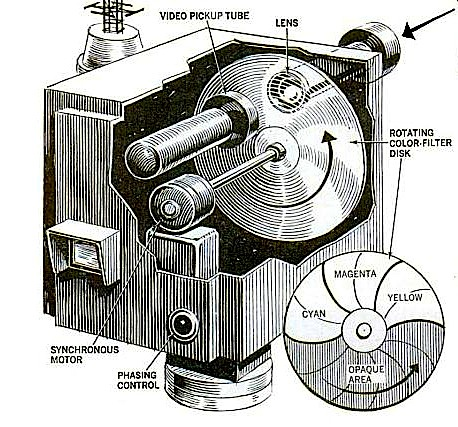
\includegraphics[scale=.55]{graphics/color_encoder.jpg}
    \caption{Butterfield color encoder \citep{Shatavsky:1968vn}}
    \label{fig:3}
\end{figure}

That the pulsed black-and-white signal produced by the Butterfield color encoder gives rise to a chromatic appearance is once again the result of the visual system integrating temporal inhomogeneities. However, these temporal inhomogeneities are not the result of spatial movement of the object of perception, but rather due to the qualitative alterations over time of a stationary object. Each involves the presentation of white and black stimuli altering at a particular temporal ratio eliciting a chromatic response in normal human perceivers. They differ in how that temporal ratio is implemented---by the motion of an object whose parts qualitatively differ or by the qualitative alteration over time of a stationary object. 

Stated so abstractly it is easy to see that there is a third possibility. If the temporal ratio that determines a given chromatic appearance can be implemented by the motion of a black and white object, the perceivers motion relative to a black and white object should do so as well. And indeed it can. Our eyes constantly scan the scene with involuntary saccades. Scanning a stationary black and white object can give rise to chromatic appearance \citep[72]{Hardin:1993kn}. Thus Sorabji claims that contemporary art provides an example:
\begin{quote}
    I also wrote about colour and vision in the 1970s. At Cornell, I had heard Edward Land, the inventor of the polaroid camera, lecture on his discovery that Newton’s theory of colour is wrong. The eye responds not to absolute wavelengths of light, but to the more complicated property of reflectance, which involves the proportions among wavelengths in the available scene. Land was able to cast on the screen at Cornell a slide showing all the colours of the garden, yet he was using wavelengths only from within the yellow waveband. I was intrigued that Goethe had also rejected Newton’s theory of colour, and praised Aristotle for his theory that the other hues are produced by combinations of the brightest and the darkest. This, according to Goethe, is the theory that any painter would accept. We had a reproduction in our hallway of a painting by Bridget Riley consisting of wavy black and white stripes. Some of our guests saw brilliant colours in it. Others merely felt giddy. I wrote to ask Bridget Riley what she thought of Goethe and Arsitotle, but this time I did not get an answer. (\citealt[13]{Sorabji:2005fk}; see also \citealt[295]{Sorabji:2022qf})
\end{quote}
The chromatic appearances that Riley's painting give rise to (see Figure~\ref{fig:4}) are the result of the visual system integrating temporal inhomogeneities that result from the eye involuntarily moving across a stationary black and white object.

\begin{figure}[htbp]
    \centering
        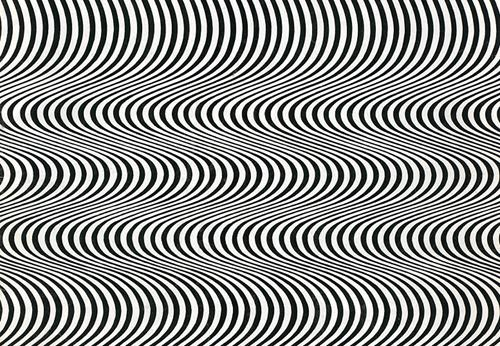
\includegraphics{graphics/current.jpg}
    \caption{Bridget Riley, \emph{Current}}
    \label{fig:4}
\end{figure}

These examples involve artifacts and technology unavailable at Aristotle's time. And while they may make plausible for \emph{us} that ratios of white and black can, sometimes at least, give rise to chromatic appearances, they could not have done so for Aristotle. What empirical observation available to Aristotle could have made vivid for him the possibility that chromatic appearances are the result of the ratio of light and dark in the perceived scene? An example discussed in the last chapter could give rise to the relevant experience. The sun is white, but it appears red when seen through fog or a cloud of smoke (\emph{De Sensu} 3 440\( ^{a} \)10--11).  The white sun, when superimposed by black particles suspended in the intervening transparent medium, looks red. The reduction of the sun's brilliance by the intervening particulate matter of the smoke results in the sun's crimson appearance. In his \emph{Theory of Colors}, Goethe repeats and elaborates Aristotle's example:
\begin{quote}
	The highest degree of light, such as that of the sun, of phosphorus burning in oxygen, is dazzling and colourless; so the light of the fixed stars is for the most part colourless. This light, however, seen through a medium but very slightly thickened, appears to us yellow. If the density of the medium be increased, or if its volume become greater, we shall see the light gradually assume a yellow-red hue, which at last deepens to a ruby-colour. \citep[\textsc{i}.10 150]{Goethe:1810uq}
\end{quote}
\begin{quotation}
	\noindent The sun seen through a certain degree of vapour appears with a yellow disk; the centre is often dazzling yellow when the edges are already red. The orb seen through a thick yellow mist appears ruby-red (as was the case in 1794, even in the north); the same appearance is still more decided, owing to the state of the atmosphere, when the scirocco prevails in the southern climates: the clouds genrally surrounding the sun in the latter case are of the same colour, which is reflected again on all objects.
	
	The red hues of morning and evening are owing to the same cause. The sun is announced by a red light, in shining through a greater mass of vapours. The higher he rises, the yellower and brighter the light becomes. \citep[\textsc{i}.10 154]{Goethe:1810uq}
\end{quotation}

What is presently important is a general feature of Aristotle's example: that a reduction of an object's brilliance can result in a chromatic appearance. That provides direct partial support for the claim that a proportion of light and dark can give rise to a chromatic appearance.

% section empirical_support (end)

\section{Parmenides} % (fold)
\label{sec:parmenides}
Theophrastus (\emph{De Sensibus} 79; DK 68\textsc{a}135) alludes to a pre-Democritean tradition according to which white and black are the primary colors, the colors in terms of which all other colors are to be explained. While Theophrastus does not name any particular thinker belonging to this tradition, one may reasonably speculate. In his notorious study, among the five ``signs of the immaturity'' of the Homeric color scheme, Gladstone cites the following:  
\begin{quote}
    The vast predominance of the most crude and elemental forms of colour, black and white, over every other, and the decided tendency to treat other colours as simply intermediate modes between these two extremes. \citep[458]{Gladstone:1858fk}
\end{quote}
One can reasonably accept Gladstone's observation about the structure of the Ho\-meric color scheme, while bracketing any conclusions about relative deficiencies in the Greek's capacity to discriminate color or about their taste in color composition. Amusingly, \citealt[162]{Platnauer:1921bh}, while tempted by Gladstone's diagnosis of color blindness among the ancient Greeks, accuses them instead of having bad taste in being insensitive to ``the qualitative differences of decomposed and partially absorbed light''. If we bracket such judgments, then arguably the pre-De\-mo\-cri\-tean tradition that Theophrastus alludes to has Homeric roots. Let us selectively examine this ancient tradition by attending to two key figures familiar to Aristotle, Parmenides and Empedocles (though the inclusion of the latter is controversial).

In the prologue to his poem, the goddess promises to reveal to Parmenides two things, the Way of Truth and the Way of Mortal Opinion. The doctrines of the latter she assures him are false; nevertheless, Parmenides must learn these too (DK 28\textsc{b}1 31). The Way of Mortal Opinion is an account of the world ``as it appears'' (DK 28\textsc{b}8 60; \citealt[155]{McKirahan:1994ve}), and the goddess presents it to Parmenides ``so that no mortal opinion may ever overtake'' him (DK 28\textsc{b}8 61; \citealt[155]{McKirahan:1994ve}). The Way of Mortal Opinion is a cosmology in the Milesian tradition, though Parmenides is not expounding the views of any particular Milesian cosmologist \citep[on Parmenides and Milesian cosmology see][]{Kahn:1994qf}. Rather, he is presenting what is, by his lights, the best account that can be given along those lines. Traditional Milesian cosmologies tend to be monistic, but the Way of Mortal Opinion posits two fundamental and irreducible principles that stand in opposition, Fire and Night or light and dark (DK 28\textsc{b}8 53--61, 28\textsc{b}9). The thought seems to be this. Having shown, in the Way of Truth, that monism is inconsistent with appearances, the Way of Mortal Opinion must posit a plurality of principles in opposition, if it is to accommodate the plurality and opposition encountered in the world as it appears in sensory experience. Or at least, this is the interpretation that Aristotle recommends:
\begin{quote}
    \ldots\ but being forced to follow the phenomena, and supposing that what is is one in formula but many according to perception, he now posits two causes and two principles, calling them hot and cold, \emph{i.e.} fire and earth. (\emph{Metaphysics} \( A \) 986\( ^{b} \) 31; Ross in \citealt[]{Barnes:1984kx})
\end{quote}

The two principles, Fire and Night, of the Way of Mortal Opinion, have attributes called ``signs'':
\begin{verse}
    For they made up their minds to name two forms,\\ 
    Of which it is not right to name one---in this they have gone astray---\\
    And they distinguished things opposite in body, and established signs\\
    Apart from one another---for one, the aetherial fire of flame,\\
    Mild, very light, the same as itself in every direction,\\
    But not the same as the other; but that other one, in itself\\
    Is opposite---dark night, a dense and heavy body.\\
    I declare to you all the ordering as it appears,\\
    So that no mortal opinion may ever overtake you.
\end{verse}
\begin{verse}
    But since all things have been named light and night\\
    And the things which accord with their powers have been assigned to these things and those,\\
    All is full of light and obscuring night together,\\
    of both equally, since neither has no share.\\
    (Parmenides, DK 28\textsc{b}8 53--9 4; \citealt[155]{McKirahan:1994ve})
\end{verse}
Like Fire and Night themselves, the attributes of these principles stand in opposition. Fire is bright, Night is dark; Fire is rare, Night is dense, and so on. These attributes are sensible qualities arrayed in opposing pairs of contraries. In contrast, the attributes of the one being of the Way of Truth are not sensible (\emph{aistheton}) but intelligible (\emph{noeton}) properties (such as limit or unity).  Fire and Night may have further attributes not listed here; much of the Way of Mortal Opinion is missing. A sense of its scope and ambition, however, is provided by Plutarch:
\begin{quote}
    But Parmenides \ldots\ has actually made a cosmic order, and by blending as elements the light and the dark produces out of them and by their operation the whole world of sense. Thus he has much to say about earth, heaven, sun, moon, and stars, and has recounted the genesis of man; and for an ancient natural philosopher---who has put together a book of his own, and is not pulling apart the book of another---he has left nothing of real importance unsaid. (Plutarch, \emph{Adversus Colotem} 1114 b--c; \citealt[231]{Einarson:1967zr})
\end{quote}

Arguably, the cosmology of Fire and Night posited by the Way of Mortal Opinion is prefigured in the prologue of the poem. On his journey to meet the goddess, Parmenides, escorted by the daughters of the Sun, travels from Night to Day:
\begin{verse}
    \ldots\ the daughters of the Sun\\
    Were hastening to escort <me> after leaving the house of Night\\
    For the light, having pushed back the veils from their heads with their hands.\\ 
    (Parmenides, DK 28\textsc{b}1 8--10; \citealt[151]{McKirahan:1994ve})
\end{verse}
But before they can meet the goddess they must pass through the gates of the roads of Night and Day:
\begin{verse}
    There are the gates of the roads of Night and Day,\\
    And a lintel and a stone threshold contains them.\\ 
    High in the sky they are filled by huge doors\\
    Of which avenging Justice holds the keys that fit them.\\
    (Parmenides, DK 28\textsc{b}1 11--13; \citealt[151]{McKirahan:1994ve})
\end{verse}
Why must Parmenides first pass through these gates before gaining an audience with the unnamed goddess? The significance of the gates can be brought out by considering the identity of Justice who holds their keys. According to the Way of Mortal Opinion, at the center of the cosmos is a goddess ``that governs all'' (DK 28\textsc{b}12)  Aëtius reports that this goddess is none other than Justice from the prologue:
\begin{quote}
	The middlemost of the mixed rings is the [primary cause] of movement and of coming into being for them all, and he calls it the goddess that steers all, the holder of the keys, Justice and Necessity. (Aëtius, DK 28\textsc{a}37; \citealt[151]{McKirahan:1994ve})
\end{quote}
While the intelligible world of the Way of Truth pertains to being, the sensible world of the Way of Mortal Opinion pertains to becoming. Justice governs all change in the sensible world by governing alternations in the mixture of Fire and Night. Parmenides in passing through the gates of the roads of Night and Day leaves the sensible world governed by alternations of Fire and Night, to the intelligible world where a goddess awaits to reveal to him the one being of the Way of Truth. Parmenides travels from the sensible world to the intelligible world, from the world of becoming to the world of being.

If, according to the Way of Mortal Opinion, the ``the whole world of sense''---in which appear ``earth, heaven, sun, moon, and stars''---is ultimately explained in terms of light and dark in opposition, then the qualities of material objects that appear in sensory experience are themselves to be explained in these terms. Since colors are qualities of material objects that appear in sensory experience, they are themselves to be explained in terms of the ``blending'' of light and dark. Whether or not Theophrastus had Parmenides in mind, Parmenides straightforwardly belongs to the pre-Democritean tradition that postulates white and black or light and dark as the primary colors.

% section parmenides (end)

\section{Empedocles} % (fold)
\label{sec:empedocles}

It is arguable that Theophrastus did in fact have Empedocles in mind when alluding to this pre-Democritean tradition. Despite extensive discussion of Empedocles' views about sensory experience and its objects, Theophrastus does not make the parallel charge against Empedocles that he makes against Democritus (\emph{De Sensibus} 79; DK 68\textsc{a}135; \citealt{Stratton:1917vn}). Moreover, as we have seen, Theophrastus complains that while Empedocles has explained the perception of white and black he has failed to explain the perception of the other hues (\emph{De Sensibus} 17; \citealt{Stratton:1917vn}). This is strong defeasible evidence that Theophrastus took Empedocles to be among the thinkers who take white and black or light and dark as the primary colors (albeit with limited success, at least by Theophrastus' lights).

In contrast with Parmenidean monism, Empedocles postulates the existence of four ``roots'' or elements---water, earth, air, and fire---and two principles---\-Love and Strife. Whereas Love, the principle of harmony, has the power to unite, Strife, the principle of disorder, has the power to divide. According to Empedocles, things are colored because of the combination of elements that result from Love overcoming Strife to the extent that it does:
\begin{verse}
    And if, concerning these things, your conviction is in any way wanting,\\
    as to how from the blending of water and earth and aither and sun\\
    the forms and colours of mortals came to be,\\
    which have now come to be, fitted together by Aphrodite.
    (DK \textsc{b}71; \citealt[74 249]{Inwood:2001ve})
\end{verse}
The forms and colors of objects we encounter in sensory experience are to be explained in terms of the combination of the elements that result from Love's influence counteracting the operation of Strife.

\citet[222]{Wright:1981zr} suggests that the reference to form and color is a deliberate echo of an earlier fragment:
\begin{verse}
    As when painters adorn votive offerings,\\
    men well-learned in their craft because of cunning,\\
    and so when they take in their hands many-coloured pigments,\\
    mixing them in harmony, some more, others less,\\
    from them they prepare forms resembling all things,
    making trees and men and women\\
    and beasts and birds and water-nourished fish\\
    and long-lived gods, first in their prerogatives.\\
    In this way let not deception overcome your thought organ\\
    that the source of mortal things, as many as have become obvious---countless---is anything else,\\
    but know these things clearly, having heard the story from a god.\\ 
    (DK \textsc{b}23; \citealt[27 231]{Inwood:2001ve})
\end{verse}
However, the two fragments seem to be making different points. Empedocles in this earlier fragment describes the generation of the objects we encounter in the sensible world by analogy with painting. Just as painters can represent everything in the sensible world by combining pigments in various proportions, Love and Strife can generate everything in the sensible world by combining the elements in various proportions. However, unlike the later fragment (DK \textsc{b}71) no specific mention is made about the colors of the generated objects or how they are the result of the combination of elements. Whereas the earlier fragment (DK \textsc{b}23) claims that a combination of a few colors suffice to represent the forms and colors encountered in the sensible world, the latter fragment (DK \textsc{b}71) claims that a combination a few elements suffice for the forms and colors encountered in the sensible world.

The painting analogy remains instructive, however. Specifically, it sheds light on the sense in which the combination of a few colors suffice to represent all the colors that appear in sensory experience. This is important since in the context of Empedocles' analogy, this is the sense in which the elements combine. And given the latter fragment (DK \textsc{b}71), the elements when combined in this sense suffice for the form and color of all things. First, observe that, despite their manifest plurality, the ``roots'' or elements are otherwise Parmenidean beings---they do not admit of alteration, growth, or decay. Change as we experience it is the result of different combinations of these unchanging elements:
\begin{verse}
    I shall tell you something else. There is no growth of any or all mortal things\\
    nor any end in destructive death,\\
    but only mixture and interchange of what is mixed\\
    exist, and growth is the name given to them by men.\\
    (DK \textsc{b}8; \citealt[21 221]{Inwood:2001ve})
\end{verse}
So for the analogy to hold, the painter's combination cannot be understood as a blending or mixture (on the model of mixing oil paint on a palette, or dissolving sugar in water). If when the elements combine they do so in a mixture, then the elements would no longer be distinguishable in the compound. But this is inconsistent with their status as Parmenidean beings. So a negative lesson, then, is that the combination as it figures in the analogy cannot coherently be understood as blending or mixture.

If combination, here, cannot coherently be understood as mixture, how, then, is it to be understood? Recent commentators have made the important suggestion that combination as it figures in the analogy should be understood in terms of the actual practices of fifth century \textsc{bc} painting \citep{Wright:1981zr,Mourelatos:1987fk,Ierodiakonou:2005fk}. However, this yields two distinct models, and as a consequence, I am less certain about the positive lessons that the analogy affords us.

Consider what is arguably the most important development of fifth century \textsc{bc} painting, the development of chiaroscuro or \emph{skiagraphia} \citep[see][]{Bruno:1977fk,Keuls:1975uq,Pemberton:1976kx}. In archaic Greek painting, figures appear outlined and uniformly colored in a two-dimensional pictorial plane. Moreover, the color of the figures tended to complement and support the overall two-dimensional composition. However, in the fifth century \textsc{bc}, the ``shadow painters'' came to emphasize, instead, lightness and darkness in organizing their compositions. There was less reliance on outlining, figures were no longer uniformly colored as primitive methods of shading were developed, and as a result, the figures began to emerge from the two-dimensional pictorial plane. To emphasize the importance of relative brightness in their composition, the shadow painters worked with a limited palette. Nevertheless, they were able to produce the appearance of a variety of colors by combining the colors of this limited palette. Importantly, there were two techniques for combining the few colors, corresponding to different periods in the development of \emph{skiagraphia}.

In \emph{De Gloria Atheniensium}, Plutarch attributes the invention of fifth century \textsc{bc} chiaroscuro to Apollodorus. In seeming contradiction to Plutarch's testimony, Quintillian claims that a student of Apollodorus, Zeuxis, invented the law of light and shadow. \citet[27--29]{Bruno:1977fk} reconciles these apparently conflicting claims by arguing that they are in fact describing distinct dramatic episodes or turning points in the development of fifth century \textsc{bc} chiaroscuro:
\begin{quote}
    The Apollodorian accomplishment and that artist's importance in the art-historical record as it has come down to us from ancient times can only be explained if he was somehow able to synthesize earlier, less successful attempts, so that a systematic relationship between chiaroscuro and color was established in some consistent manner. Such an accomplishment and nothing less (when we consider the rather late fifth-century dates we must assume for the career of this artist) might have struck the imagination of the ancient viewer as anything so dramatic as an ``invention''. Then Zeuxis, who ``walked through the doors'' that his teacher, Apollodorus, had opened, must have been able to develop more sophisticated variations of the earlier methods. In his own mature work, he must have departed in some striking manner from the system of shading that had characterized his master's pictures; the likelihood is that Zeuxis invented a kind of chiaroscuro in which the relationship of color to dark and light was definitely altered, in which shading assumed a more dominant role and the nuances of coloring and brushwork became more and more complex, perhaps more ``painterly''. \citep[29]{Bruno:1977fk}
\end{quote}
What is presently relevant is that different methods of color combination are associated with these distinct dramatic episodes in the development of fifth century \emph{bc} chiaroscuro.

In \emph{De Gloria Atheniensium}, not only does Plutarch attribute the invention of \emph{skiagraphia} to Apollodorus, but also the invention of a method of color combination. Specifically, working with a limited palette, Apollodorus would produce novel colors by overlaying washes of different colors. A four-color palette was common in the fifth century \textsc{bc} and  Pliny reports that it reached its finest expression in fourth century \textsc{bc} painting:
\begin{quote}
	Four colours only---white from Melos, Attic yellow, red from Sinope on the Black Sea, and the black called ``atramentum''---were used by Apelles, Aetion, Melanthios and Nikomachos in their immortal works. (\emph{Historia Naturalis} 35 50; \citealt[97]{Jex-Blake:1896uq})
\end{quote}
The Alexander mosaic depicting the Battle of Isis is a Roman work from the first century \textsc{bc} that is a copy of a Greek four-color painting. Pliny (\emph{Historia Naturalis} 35 110; \citealt[143]{Jex-Blake:1896uq}) attributes the original four-color painting to Philoxenos of Eretria ``who painted for king Kassander the battle between Alexander and Dareios, a picture second to none.'' The Alexander mosaic gives us a sense of the naturalistic skin tones that could be achieved with four-color painting (see figure~\ref{fig:alexander}). However, being a mosaic, it is in this respect misleading---the fundamental method of color combination in mosaics is the juxtaposition of differently colored tiles as opposed to the overlaying of differently colored washes (though of course these methods can be combined). Sellers suggests that for a better sense of what can be accomplished with only four colors we need only consider Titian's ``Christ crowned with thorns'' in the Louvre (see figure~\ref{fig:christ}; \citealt[97 note]{Jex-Blake:1896uq}; for a revealing if idiosyncratic account of the Greek four-color palette and Venetian painting see \citealt{Pavey:1956fk}). So one way of combining colors is by overlaying differently colored washes, that is, by overlap.

\begin{figure}[htbp]
    \centering
        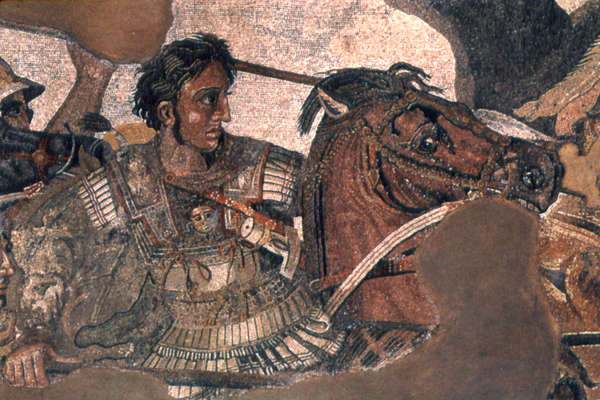
\includegraphics[scale=0.70]{graphics/alexander.jpg}
    \caption{Detail of the Alexander Mosaic, 1st century \textsc{bc}}
    \label{fig:alexander}
\end{figure}
\begin{figure}[htbp]
    \centering
        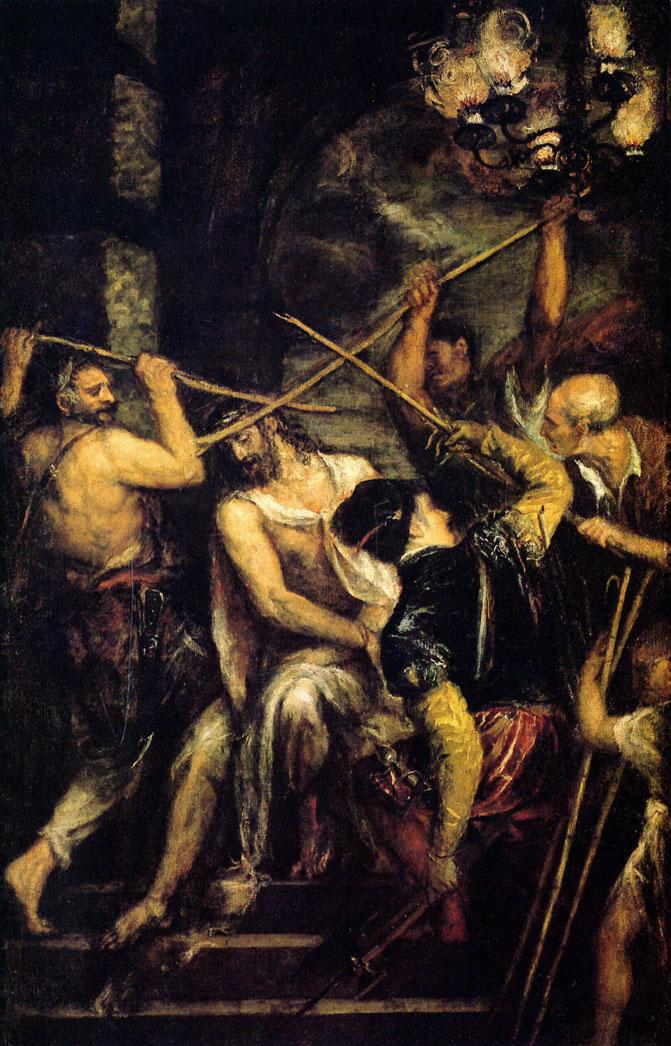
\includegraphics[scale=0.5]{graphics/christ.jpg}
    \caption{Titian, ``Christ Crowned with Thorns'', 1570}
    \label{fig:christ}
\end{figure}

We have seen \citet[29]{Bruno:1977fk} claim that in the sophisticated chiaroscuro inaugurated by Zeuxis ``shading assumed a more dominant role and the nuances of coloring and brushwork became more and more complex, perhaps more `painterly'.'' A sense of this more ``painterly'' style can be seen, according to Bruno, in the figure of Rhadmanthys painted on the facade of the tomb of Lefkadia (see figure~\ref{fig:tomb}):
\begin{quote}
    A dark is not just an area of darker pink or brown flesh tones; it has blues and greens running through it and a complex system of overlapping tones in which every individual stroke is a slightly different color. Color accidents, produced by quick, overlapping brushstrokes, abound throughout the work and are accidents upon which the artist relied. \citep[25]{Bruno:1977fk}
\end{quote}
In the late development of fifth century \textsc{bc} chiaroscuro, as light and dark come to further dominate the compositional scheme, the relationship between form and color became complicated. Whereas earlier forms of chiaroscuro would use one color for shaded parts of a figure, later forms would use a variety of colors, their choice controlled more by relative brightness than hue. The effect of this more complicated scheme may without too much risk of anachronism be described as proto-impressionistic. However, \emph{pace} \citet{Keuls:1975uq}, I do not think that the literary and archeological evidence supports the attribution of nineteenth century ``divisionist'' technique to fifth century \textsc{bc} painters \citep[see][]{Pemberton:1976kx}. However, there need be no ancient predecessor of Suerat in fifth century \textsc{bc} painting for there to be a method of color combination that involved not the overlap but the juxtaposition of color.

\begin{figure}[htbp]
    \centering
        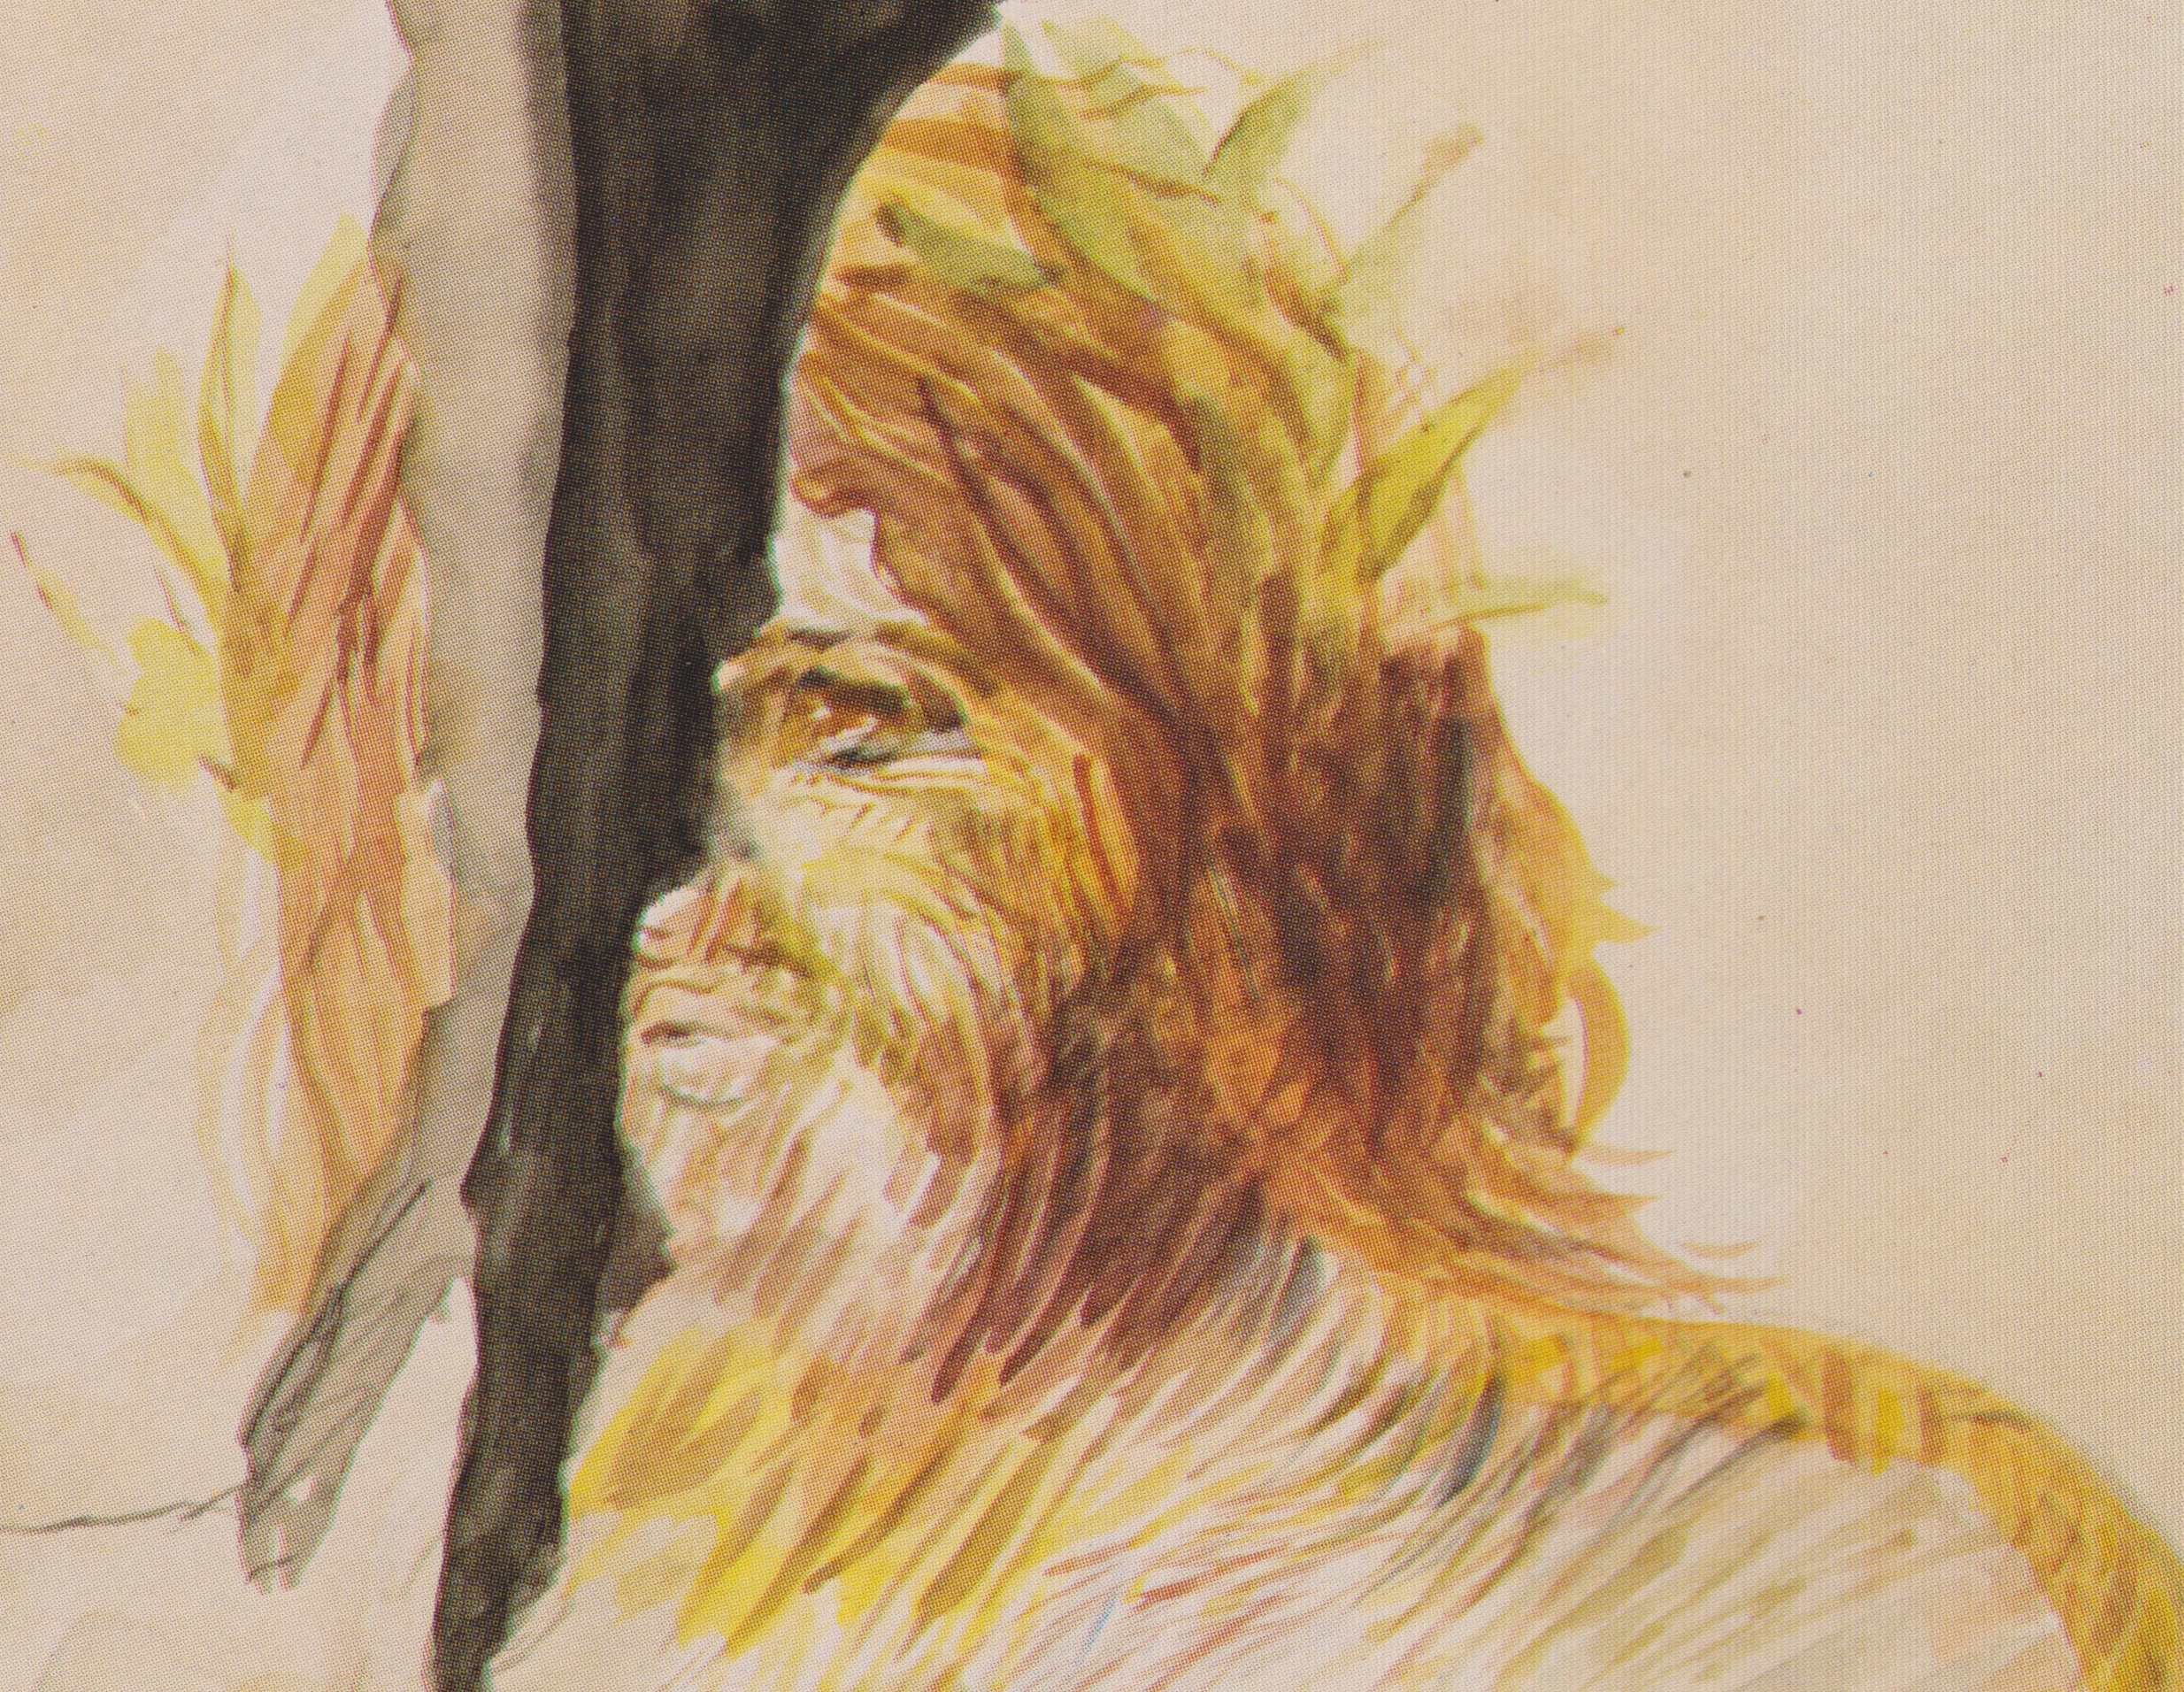
\includegraphics[scale=1]{graphics/tomb.jpeg}
    \caption{Victor Bruno's watercolor sketch of Rhadamanthys at the tomb of Lefkadia}
    \label{fig:tomb}
\end{figure}

We have seen that combination in Empedocles' painting analogy cannot be understood in terms of mixture. If the sense in which painters combine colors in various proportions to represent the forms of all things is analogous to the sense in which the opposing forces of Love and Strife combine the elements in various proportions, then the metaphysical status of the elements rules out understanding the combination as mixture, since the elements would be indistinguishable in the compound. Fifth century \textsc{bc} painting, however, provides us with two further models. Perhaps the combination could be understood, not in terms of mixture, but in terms of overlap or juxtaposition. 

In \emph{On Generation and Corruption}, Aristotle claims that the Empedoclean elements combine by means of juxtaposition and compares the compound to a brick structure:
\begin{quote}
    For how is the manner of their coming-to-be to be conceived by those who maintain a theory like Empedocles? They must conceive it as \emph{composition}---just as a wall comes-to-be out of bricks and stones: and the `Mixture', of which they speak, will be composed out of the `elements', these being preserved in it unaltered but with their small particles juxtaposed. (\emph{On Generation and Corruption}, \textsc{ii} 7 334\( ^{a} \)26--30)
\end{quote}
The Aristotelian interpretation is supported by Galen's testimony:
\begin{quote}
     For Empedocles says that we, and all the other earthly bodies, are generated from the same elements assumed by Hippocrates, and these elements are not combined with each other, but, as small pieces, stand next to each other, touching. (\emph{Hippocratis De Naturis Homina Commentaria} 15 49; DK 31\textsc{a}43)
\end{quote}
And Galen compares the combination of Empedoclean elements to a powder consisting of finely ground metals (\emph{Hippocratis De Naturis Homina Commentaria} 15 32; DK 31\textsc{a}34). Further support for the Aristotelian interpretation comes from an Empedoclean metaphor. Thus he speaks of Love's influence in combining the elements as ``the divine glues of harmony'' (DK \textsc{b}96; \citealt[62 245]{Inwood:2001ve}). The metaphor of gluing suggests that the elements ``are not combined with each other, but, as small pieces, stand next to each other, touching''.

If we accept the Aristotelian interpretation, then the combination of the elements should be understood on the model of juxtaposition. So, for the analogy to hold, the painter's method of combining colors must itself be understood on the model of juxtaposition, a method arguably associated with the late chiaroscuro inaugurated by Zeuxis and whose influence can be seen in the tomb of Lefkadia. However, Zeuxis' achievement is too late---it arguably post-dates the composition of Empedocles poem(s).  \citet[38--39]{Wright:1981zr}, following \citet[148]{Guthrie:1965ys}, associates the painter's combining of colors with Apollodorus and Greek four-color painting. Wright proposes to understand the painter's combining the colors in various proportions with the technique of color combination associated with Greek four-color painting, but that technique works by overlap, not juxtaposition. It is this mismatch that makes me uncertain what positive lessons Empedocles' analogy can provide us about the painter's method of combining colors. It is possible that Aristotle and Galen are right that the Empedoclean combination of elements should be understood on the model of juxtaposition \emph{and} that Guthrie and Wright have correctly interpreted the painter's combination of colors in terms of overlaying washes of different colors. In which case, the analogy, considered by itself, could serve only to establish the original negative lesson. The combination of the elements is like the combination of the colors in that neither should be understood in terms of blending or mixture. Rather, as it turns out, they work on the models of juxtaposition and overlap, respectively.

How does the combination of elements in various proportions result in the colors of things as they appear in sensory experience? According to Aëtius, four colors---white, black, red, and yellow (the Greek four-color palette)---are assigned to the elements, though Aëtius does not say which color belongs with which element. Partly on this basis some commentators attribute to Empedocles the view that the four elements have four unique colors (\citealt[217]{Cherniss:1935fk}, \citealt[152-3]{Siegel:1959fk}). This would be the basis of the desired explanation if the colors of compound bodies were explained in terms of the colors of their constituent elements. Notice that, on such an explanation, white, black, red, and yellow would be the primary colors---the view that Theophrastus criticizes Democritus for holding (modulo the substitution of yellow for green).  However, the fragments as they come down to us provide no direct support for this interpretation \citep[see][]{Ierodiakonou:2005fk}. While Empedocles claims that fire is white and water is black, no specific colors are associated with the other elements. 

I believe that it is more likely that Empedocles is following Parmenides in taking white and black or light and dark as the primary colors. As we will see, this interpretation coheres well with Theophrastus' account of Empedocles' theory of color vision. To illustrate this alternative, let us consider three fragments where Empedocles' associates white with fire and black with water.

Aristotle (\emph{De Anima} (410\( ^{a} \)1)) cites the following Empedoclean fragment to illustrate the way in which compound bodies do not merely consist in their constituent elements, but must be combined in a certain proportion:
\begin{verse}
    And pleasant earth in her well-built channels\\
    received two parts of gleaming Nestis out of the eight\\
    and four of Hephaistos; and they become white bones\\
    fitted together with the divine glues of harmony.\\
    (DK \textsc{b}96; \citealt[62 245]{Inwood:2001ve})
\end{verse}
Nestis is a Sicilian water-goddess, and Hephaistos is associated with fire. Thus, according to the fragment, bone is the result of Love's combining four parts fire with two parts earth and two parts water. Though some commentators take Nestis to refer to water and air, perhaps under the influence of the general conviction that all four elements are present in every compound body \citep[209 n2]{Wright:1981zr}. On this alternative interpretation, the proportion of elements in bone is four parts fire, two parts earth, one part water, and one part air. On either interpretation, Empedocles seems to be explaining the whiteness of bones in terms of the preponderance of fire in their constituent elements. If we combine this thought with the answer in the style of Gorgias presented in the \emph{Meno}, then the idea would be that bone, due to the preponderance of fire in its composition, gives off a fiery effluence. This fiery effluence, due to its distinctive magnitude, enters the fire passages in the membrane of the eye and so is made palpable to sight. In this way the whiteness of the bone is manifest in sensory experience.

That the color of fire is white is further confirmed by a fragment according to which the sun is white or bright while rain is black or dark:
\begin{verse}
    But come! Gaze on this witness to my previous words,\\
    if anything was in my previous [remarks] left wanting in form:\\
    the sun, bright to look on and hot in every respect,\\
    and the immortals which are drenched in heat and shining light,\\
    and rain, in all things dark and cold;\\
    and there flow from the earth things dense and solid.\\
    (DK \textsc{b}21 1--6; \citealt[26 1--6, 229]{Inwood:2001ve})
\end{verse}
Not only then is fire, in the guise of the sun, light, but the fragment associates another element with a specific color: The water which composes the rain is dark.

That fire and water are the elemental equivalents of light and dark is further confirmed by a fragment cited by Plutarch:
\begin{verse}
    And in the depths of the river a black colour is produced by the shadow,\\
    and in the same way it is observed in cavernous grottoes.\\
    (DK \textsc{b}94; \citealt[105 261]{Inwood:2001ve})
\end{verse}
The fragment only explicitly claims that the depths of the river is black, but Plutarch cites the fragment in answer to the question ``Why does the surface of the water look white and the depths look black?'':
\begin{quote}
    Is it because the depth is the mother of blackness inasmuch as it blunts and weakens the sun's rays before they can get to it? But since the surface is immediately affected by the sun, it is reasonable that it receives the gleam of light.  (\emph{Historia Naturalis} 39; \citealt[\textsc{ctxt}-87 137--138]{Inwood:2001ve})
\end{quote}
If we accept Plutarch's attribution of this explanation to Empedocles, this supports the elemental equivalence of fire and water with light and dark. It also strikingly prefigures the central thought of Aristotle's account of the generation of the hues. Water is by nature black. However, the color that water appears to have can change depending on whether and to what degree it is illuminated. The surface of water looks white, at least in the shifting pattern of reflective highlights. The water near to the surface, where it is not as brightly illuminated, looks blue. And the depths of the river, where the sun's rays fail to penetrate, looks black. (Compare Aristotle's claim that the sea is an imperfectly transparent medium that appears differently near or far \emph{De Sensu} \textsc{iii} 439\( ^{b} \)1--3 and his claim that water looks darker the deeper and less transparent it is \emph{De Generatione Animalium} 779\( ^{b} \)27--33, 780\( ^{b} \)8.) The different colors---white, blue, and black---are due to different different proportions of fire and water. In the shifting pattern of reflective highlights, there is a preponderance of fire and this results in a brilliant appearance; whereas, in the depth of the river, there is a preponderance of water (and perhaps no fire at all) and this results in a dark appearance. In the shallows of the river, due to a more equitable combination of fire and water, a blue appearance is manifest.

Accepting Plutarch's attribution, and generalizing it, thus results in the following picture: White and black, like hot and cold, are sensible qualities paired with their contrary. And like hot and cold, white and black are the endpoints of an ordered range of sensible qualities. That the range is ordered as a continuum is a further claim. Aristotle, for one, denies it (\emph{De Sensu} \textsc{vi}). Blue is a sensible quality located somewhere between the extremes of white and black as is every other color. Blue is perhaps more dark than light just as yellow is more light than dark. In this regard, Empedocles' theory shares a feature with the Homeric color scheme of which \citet[458]{Gladstone:1858fk} complained, namely, ``the decided tendency to treat other colours as simply intermediate modes between these two extremes'', that is, ``the crude and elemental forms of colour, black and white''. Moreover, the relevant proportion of light and dark is determined by the substance's elemental composition. The proportion of light and dark that results in the blue of the river's shallows is determined by the proportion of fire and water in its composition. Specifically, the fiery emission of the sun penetrates to some degree the shallows of the river, and it is the resulting proportion of fire and water that determines the proportion of light and dark of which the shallows partake. 

This constitutes a means for addressing one of Theophrastus' complaints. Theo\-phrastus concedes that on Empedocles' account, the perception of white and black is relatively straightforward. In the membrane of the eye there are alternating passages of fire and water. White effluences emitted from distal objects are assimilated by fire passages, black effluences are assimilated by water passages, and so each is made palpable to the organ of sight. But how, on this model, is the perception of the chromatic hues to be explained? Theophrastus complains that Empedocles owes us an explanation but has failed to provide one:
\begin{quote}
	Now since, for him, the eye is composed of fire and of its opposite, it might well recognize white and black by means of what is like them; but how could it become conscious of gray and the other compound colours? For he assigns <their perception> neither to the minute passages of fire nor to those of water nor to others composed of both these elements together. Yet we see the compound colours no whit less than we do the simple. (\emph{De Sensibus} 17; \citealt{Stratton:1917vn})
\end{quote}

The elemental composition of a distal object, specifically, its proportion of fire and water, determines the amount of fiery and watery effluences it emits. Fiery effluences are white. Watery effluences are black. A purely white object, such as a noon sun on a clear summer's day, emits only fiery effluences. A purely black object, such as the river's depths, emits only watery effluences. Objects with chromatic hues emit a proportion of fiery and watery effluences corresponding the proportion of fire and water in its elemental composition. Thus the river's shallows emits a proportion of fiery and watery effluences (the fiery effluences being the sun's contribution in penetrating the river). These fiery and watery effluences are assimilated, respectively, by the fire and water passages in the membrane of the eye. And, arguably at least, it is the proportion of fire and water assimilated that gives rise to the perception of blue. 

Theophrastus complained that Empedocles assigns the perception of compound colors ``neither to the minute passages of fire nor to those of water nor to others composed of both these elements together.'' It is true that the perception of blue is not assigned to the fire passages in the eye's membrane, nor to its water passages. Whether it is explained in terms of ``others composed of both these elements'' depends on what exactly Theophrastus means here. Perhaps he means that just as there are fire and water passages in the membrane of the eye, there are other passages, as well, that are commensurate with effluences compounded out of fire and water. So understood, Theophrastus is right not attribute this doctrine to Empedocles. However, there is another alternative. The passages in the membrane of the eye consist solely of alternating fire and water passages. There are no other kinds of passages to be found. A chromatic hue is just the proportion of fiery and watery effluence emitted by a distal object, and its perception is the resulting proportion of assimilated fire and water being made palpable to the organ of sight. Like all things on earth and in heaven, at least in a certain stage of the cosmic cycle, the chromatic hues and their perception are the result of Aphrodite's Love, the principle of harmony, counteracting the operation of Strife. 

% section empedocles (end)

% chapter light_and_dark (end)
%!TEX root = /Users/markelikalderon/Documents/Git/formwithoutmatter/formwithoutmatter.tex
\chapter{The Generation of the Hues} % (fold)
\label{cha:the_generation_of_the_hues}

\section{Light and Dark} % (fold)
\label{sec:introduction}
The presence of the fiery substance illuminates the potentially transparent me\-di\-um. White (\emph{leukon}) corresponds to the presence of this determinant of what is actually transparent. Conversely, black (\emph{melaton}) corresponds to its absence. The absence of the fiery substance darkens the potentially transparent medium. White and black are thus associated with a fundamental condition on the visibility of remote external particulars. No doubt in part because of this Aristotle attempts to explain the other hues in terms of the ratio of white and black. He considers three such accounts, in terms of (1) juxtaposition, (2) overlap, and (3) mixture, advocating the third. On all three accounts chromatic hues are determined by white and black in various ratios, the accounts differing only in how these ratios are implemented. 

The fundamental idea common to all three accounts can seem surprising. How can the ratio of white and black result in something appearing red? Would it not instead appear gray? Thus \citet[210]{Hett:1936fk} writes that Aristotle's ``doctrine could hardly have survived a few experiments with pigments''. If Aristotle's account were disconfirmable by elementary experiments with pigment mixtures, then why did he not investigate the matter? Was it merely to avoid Plato's charge of impiety?
\begin{quote}
    There will be no difficulty in seeing how and by what mixtures the colors derived from these are made according to the rules of probability. He, however, who should attempt to verify all this by experiment would forget the difference between human and divine nature. For God only has the knowledge and also the power which are able to combine many things into one and again resolve the one into many. But no man either is or ever will be able to accomplish either the one or the other operation. (Plato, \emph{Timaeus} 68d)
\end{quote}
Aristotle's account of the generation of the hues may be surprising, but it would be wrong to prematurely dismiss it. 

The first thing to observe is that \emph{leukon} and \emph{melaton} are better understood as light and dark, rather than white and black. There is a general tendency in Greek color vocabulary to classify colors in terms of relative brightness rather than hue \citep[see][]{Gladstone:1858fk,Platnauer:1921bh,Osbourne:1968vn,Lloyd:2007fk}. Traces of such a usage exist in English. Thus we speak of white wine and white people, though neither are white in hue. Similarly neither black people nor black grapes are black in hue. This usage in English, however, does not seem to be perfectly general but is rather lexically determined. It is not the case that ``white'' can be interpreted in terms of relative brightness instead of hue when applied to just any noun. The availability of such an interpretation seems to be limited to the adjective's application to certain nouns. The more general usage in Greek is philosophically significant, for it transforms Aristotle's claim. Aristotle is not claiming that the hues are determined by the ratio of white and black, but that they are determined by the ratio of light and dark. Experiments with pigment mixtures are irrelevant to the truth of this latter claim. Thus, Aristotle need not have risked Plato's charge of impiety as Hett recomends. Not only is the thought that the hues are determined by the ratio of light and dark not disconfirmable by impious experimentation, it is independently plausible. Indeed, as I will argue below, it is an ancient prefiguration of modern reflectance theories \citep[see][]{Hilbert:1987jq}.

Two further considerations are relevant. First, there are a range of observable phenomena that support Aristotle's fundamental claim that a ratio of white and black or light and dark can give rise to chromatic appearances. Importantly, Aristotle himself provides an example. Second, Aristotle's account has ancient precedent. Thus when Theophrastus discusses Democritus's view that there are four primary colors (understood as simple colors in terms of which all other colors are to be explained), he contrasts it with the then dominant view that white and black are the two primary colors:
\begin{quote}
    But first of all, his increase of the number of primaries presents a difficulty; for the other investigators propose white and black as the only simple colours. (\emph{De Sensibus} 79; DK 68\textsc{a}135; \citealt{Stratton:1917vn})
\end{quote}
It is reasonable to suppose that Aristotle's account of the generation of the hues draws on this pre-Democritean tradition. Before discussing Aristotle's account of the generation of the hues, then, I will review some empirical support for its central idea, and will discuss the precedent for this doctrine in Parmenides and Empedocles.

% section introduction (end)

\section{Empirical Support} % (fold)
\label{sec:empirical_support}
In 1894, an English toy maker, Charles Benham, devised a top adorned with a black and white pattern (see Figure~\ref{fig:2}). Sold through Messrs. Newton and Co., an announcement of the ``Artificial Spectrum Top'' was published in \emph{Nature}:
	\begin{quote}
		The top consists of a disc, one half of which is black, while the other half has twelve arcs of concentric circles drawn upon it. Each arc subtends an angle of forty-five degrees. In the first quadrant there are three such concentric arcs, in the next three more, and so on; the only difference being that the arcs are parts of circles of which the radii increase in arithmetical progression. Each quadrant thus contains a group of arcs differing in length from those of the other quadrants. The curious point is that when this disc is revolved, the impression of concentric circles of different colors is produced upon the retina. If the direction of rotation is reversed, the order of these tints is also reversed. \citep{Benham:1894kx}
	\end{quote}
Specifically, if rotated clockwise, the innermost arcs form reddish rings, the next greenish rings, the next light blue rings, and the outermost arcs form violet rings. If rotated counterclockwise, the pattern is reversed with the innermost arcs now forming violet rings and the outermost reddish rings. The apparent colors of Benham's spinning disk are the ``subjective colors'' first described by \citep{Fechner:1838vn} and, hence, are also sometimes described as ``Fechner-Benham colors''.

\begin{figure}[ht]
    \begin{center}
        \begin{tikzpicture}
			\draw (0,0) circle (4cm);
			\filldraw[fill=black] (0,0) -- (4cm,0cm) arc (0:-180:4cm) --cycle;
			\draw[line width=5pt] (canvas polar cs:angle=0,radius=0.25cm) arc (0:45:0.25cm);
			\draw[line width=5pt] (canvas polar cs:angle=0,radius=0.50cm) arc (0:45:0.50cm);
			\draw[line width=5pt] (canvas polar cs:angle=0,radius=0.75cm) arc (0:45:0.75cm);
			\draw[line width=5pt] (canvas polar cs:angle=45,radius=1.25cm) arc (45:90:1.25cm);
			\draw[line width=5pt] (canvas polar cs:angle=45,radius=1.50cm) arc (45:90:1.50cm);
			\draw[line width=5pt] (canvas polar cs:angle=45,radius=1.75cm) arc (45:90:1.75cm);
            \draw[line width=5pt] (canvas polar cs:angle=90,radius=2.25cm) arc (90:135:2.25cm);
			\draw[line width=5pt] (canvas polar cs:angle=90,radius=2.50cm) arc (90:135:2.50cm);
			\draw[line width=5pt] (canvas polar cs:angle=90,radius=2.75cm) arc (90:135:2.75cm);
			\draw[line width=5pt] (canvas polar cs:angle=135,radius=3.25cm) arc (135:180:3.25cm);
			\draw[line width=5pt] (canvas polar cs:angle=135,radius=3.50cm) arc (135:180:3.50cm);
			\draw[line width=5pt] (canvas polar cs:angle=135,radius=3.75cm) arc (135:180:3.75cm);
		\end{tikzpicture}
    \end{center}
    \caption{The Benham Disk or ``Artificial Spectrum Top''}
    \label{fig:2}
\end{figure}

Consider a puzzling aspect of the subjective colors of the Benham disk. Each of the spinning arcs reflect light with the same spectral content and with equal average luminance. In advance of observing the spinning disk, one might reasonably expect the spinning arcs to appear as gray rings of equal brightness. Why, then, do the rings appear reddish, greenish, light blue, and violet? The subjective colors of the Benham disk are not completely understood \citep[for a review of some of the color science see][]{Campenhausen:1995yq}. However, this much is clear: The innermost ring appearing reddish is the result of the visual system integrating temporal inhomogeneities presented by the spinning disk. Presentations of black and white stimuli altering at a particular temporal ratio elicits a chromatic response in normal human perceivers. 

This basic principle was used in a prototype of color television \citep[]{Butterfield:1968uq,Butterfield:1970kx}. Developed by James F. Butterfield (who studied philosophy at the University of Chicago as an undergraduate), the broadcasting system consists of the Butterfield color encoder that produces a monochromatic signal that when broadcast and displayed on a black-and-white monitor presents a chromatic appearance. The Butterfield encoder extracts a monochromatic signal from the colored scene by passing the light from the scene through cyan, magenta, and yellow filters. The filters themselves are arranged in, what is in effect, a modified Benham Disk (see Figure~\ref{fig:3}). The bottom half of the filter is opaque with the colored filters fanned across the top half. The filters thus form a disk which is rotated. A colored object will appear black when seen through a filter of a complementary color. This and the opaque half of the rotating disk produces a pulsed black-and-white signal that elicits a chromatic response in normal human perceivers. The system produced good skin tones but unmixed hues, especially red, tended to flicker. The initial public demonstration was, by all accounts, startling:
\begin{quote}
    When electronic color was first publicly demonstrated in the Los Angeles area over KNXT, no prior announcement had been made at the request of a soft-drink manufacturer sponsoring the test. The beverage firm wanted its color commercials to be a complete surprise to viewers of black-and-white receivers. And, the telecasts were that, to say the very least. Within hours of the electronic-color broadcast, thousands of viewers began asking the same question, ``What happened? Did I really see color on my black-and-white receiver? Or am I having hallucinations?'' \citep[]{Griffin:1968fk}
\end{quote}
The power to demand such attention did not go unnoticed. The final public demonstration was an Eva Perón political advertisement.

\begin{figure}[htbp]
    \centering
        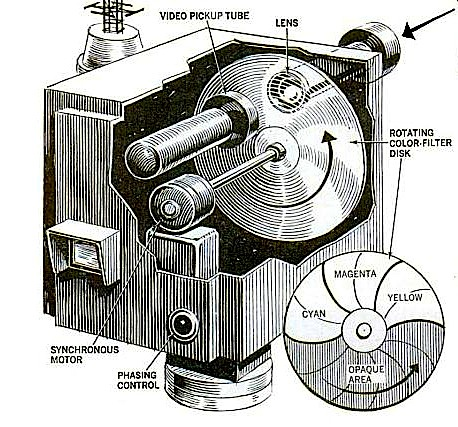
\includegraphics[scale=.55]{graphics/color_encoder.jpg}
    \caption{Butterfield color encoder \citep{Shatavsky:1968vn}}
    \label{fig:3}
\end{figure}

That the pulsed black-and-white signal produced by the Butterfield color encoder gives rise to a chromatic appearance is once again the result of the visual system integrating temporal inhomogeneities. However, these temporal inhomogeneities are not the result of spatial movement of the object of perception, but rather due to the qualitative alterations over time of a stationary object. Each involves the presentation of white and black stimuli altering at a particular temporal ratio eliciting a chromatic response in normal human perceivers. They differ in how that temporal ratio is implemented---by the motion of an object whose parts qualitatively differ or by the qualitative alteration over time of a stationary object. 

Stated so abstractly it is easy to see that there is a third possibility. If the temporal ratio that determines a given chromatic appearance can be implemented by the motion of a black and white object, the perceivers motion relative to a black and white object should do so as well. And indeed it can. Our eyes constantly scan the scene with involuntary saccades. Scanning a stationary black and white object can give rise to chromatic appearance \citep[72]{Hardin:1993kn}. Thus Sorabji claims that contemporary art provides an example:
\begin{quote}
    The English painter, Bridget Riley, has produced pictures in which black and white are juxtaposed, in long ribbons \ldots\ When people look at these black and white ribbons, many are able to see all sorts of colours appearing. \citep[295]{Sorabji:2022qf}
\end{quote}
These chromatic appearances are the result of the visual system integrating temporal inhomogeneities that result from the eye involuntarily moving across a stationary black and white object.

These examples involve artifacts and technology unavailable at Aristotle's time. And while they may make plausible for \emph{us} that ratios of white and black can, sometimes at least, give rise to chromatic appearances, they could not have done so for Aristotle. What empirical observation available to Aristotle could have made vivid for him the possibility that chromatic appearances are the result of the ratio of light and dark in the perceived scene? An example discussed in the last chapter could give rise to the relevant experience. The sun is white, but it appears red when seen through fog or a cloud of smoke (\emph{De Sensu} 3 440\( ^{a} \)10--11).  The white sun, when superimposed by black particles suspended in the intervening transparent medium, looks red. The reduction of the sun's brilliance by the intervening particulate matter of the smoke results in the sun's crimson appearance. What is presently important is a general feature of Aristotle's example: that a reduction of an object's brilliance  can result in a chromatic appearance. That provides direct partial support for the claim that a proportion of light and dark can give rise to a chromatic appearance. % In this regard, the point of Aristotle's example in its context, that the red appearing proportion of light and dark is the result of overlap or sumperimposition, is of less importance.  

% section empirical_support (end)

\section{Parmenides} % (fold)
\label{sec:parmenides}
Theophrastus (\emph{De Sensibus} 79; DK 68\textsc{a}135) alludes to a pre-Democritean tradition according to which white and black are the primary colors, the colors in terms of which all other colors are to be explained. While Theophrastus does not name any particular thinker belonging to this tradition, one may reasonably speculate. In his notorious study, among the five ``signs of the immaturity'' of the Homeric color scheme, Gladstone cites the following:  
\begin{quote}
    The vast predominance of the most crude and elemental forms of colour, black and white, over every other, and the decided tendency to treat other colours as simply intermediate modes between these two extremes. \citep[458]{Gladstone:1858fk}
\end{quote}
One can reasonably accept Gladstone's observation about the structure of the Ho\-meric color scheme, while bracketing any conclusions about relative deficiencies in the Greek's capacity to discriminate color. (Amusingly, \citealt[162]{Platnauer:1921bh}, while tempted by Gladstone's diagnosis of color blindness among the ancient Greeks, accuses them instead of having bad taste in in being insensitive to ``the qualitative differences of decomposed and partially absorbed light''.) If we do, then arguably the pre-De\-mo\-cri\-tean tradition that Theophrastus alludes to has Homeric roots. Let us selectively examine this ancient tradition by attending to two key figures familiar to Aristotle, Parmenides and Empedocles (though the inclusion of the latter is controversial).

In the prologue to his poem, the goddess promises to reveal to Parmenides two things, the Way of Truth and the Way of Mortal Opinion. The doctrines of the latter she assures him are false; nevertheless, Parmenides must learn these too (DK 28\textsc{b}1 31). The Way of Mortal Opinion is an account of the world ``as it appears'' (DK 28\textsc{b}8 60; \citealt[155]{McKirahan:1994ve}), and the goddess presents it to Parmenides ``so that no mortal opinion may ever overtake'' him (DK 28\textsc{b}8 61; \citealt[155]{McKirahan:1994ve}). The Way of Mortal Opinion is a cosmology in the Milesian tradition, though Parmenides is not expounding the views of any particular Milesian cosmologist \citep[on Parmenides and Milesian cosmology see][]{Kahn:1994qf}. Rather, he is presenting what is, by his lights, the best account that can be given along those lines. Traditional Milesian cosmologies tend to be monistic, but the Way of Mortal Opinion posits two fundamental and irreducible principles that stand in opposition, Fire and Night or light and dark (DK 28\textsc{b}8 53--61, 28\textsc{b}9). The thought seems to be this. Having shown, in the Way of Truth, that monism is inconsistent with appearances, the Way of Mortal Opinion must posit a plurality of principles in opposition, if it is to accommodate the plurality and opposition encountered in the world as it appears in sensory experience. Or at least, this is the interpretation that Aristotle recommends:
\begin{quote}
    \ldots\ but being forced to follow the phenomena, and supposing that what is is one in formula but many according to perception, he now posits two causes and two principles, calling them hot and cold, \emph{i.e.} fire and earth. (\emph{Metaphysics} \( A \) 986\( ^{b} \) 31; Ross in \citealt[]{Barnes:1984kx})
\end{quote}

The two principles, Fire and Night, of the Way of Mortal Opinion, have attributes called ``signs'':
\begin{verse}
    For they made up their minds to name two forms,\\ 
    Of which it is not right to name one---in this they have gone astray---\\
    And they distinguished things opposite in body, and established signs\\
    Apart from one another---for one, the aetherial fire of flame,\\
    Mild, very light, the same as itself in every direction,\\
    But not the same as the other; but that other one, in itself\\
    Is opposite---dark night, a dense and heavy body.\\
    I declare to you all the ordering as it appears,\\
    So that no mortal opinion may ever overtake you.
\end{verse}
\begin{verse}
    But since all things have been named light and night\\
    And the things which accord with their powers have been assigned to these things and those,\\
    All is full of light and obscuring night together,\\
    of both equally, since neither has no share.\\
    (Parmenides, DK 28\textsc{b}8 53--9 4; \citealt[155]{McKirahan:1994ve})
\end{verse}
Like Fire and Night themselves, the attributes of these principles stand in opposition. Fire is bright, Night is dark; Fire is lightweight, Night is heavy, and so on. These attributes are sensible qualities arrayed in opposing pairs of contraries. In contrast, the attributes of the one being of the Way of Truth are not sensible (\emph{aistheton}) but intelligible (\emph{noeton}) properties (such as form or unity).  Fire and Night may have further attributes not listed here; much of the Way of Mortal Opinion is missing. A sense of its scope and ambition, however, is provided by Plutarch:
\begin{quote}
    But Parmenides \ldots\ has actually made a cosmic order, and by blending as elements the light and the dark produces out of them and by their operation the whole world of sense. Thus he has much to say about earth, heaven, sun, moon, and stars, and has recounted the genesis of man; and for an ancient natural philosopher---who has put together a book of his own, and is not pulling apart the book of another---he has left nothing of real importance unsaid. (Plutarch, \emph{Adversus Colotem} 1114 b--c; \citealt[231]{Einarson:1967zr})
\end{quote}

Arguably, the cosmology of Fire and Night posited by the Way of Mortal Opinion is prefigured in the prologue of the poem. On his journey to meet the goddess, Parmenides, escorted by the daughters of the Sun, travels from Night to Day:
\begin{verse}
    \ldots\ the daughters of the Sun\\
    Were hastening to escort <me> after leaving the house of Night\\
    For the light, having pushed back the veils from their heads with their hands.\\ 
    (Parmenides, DK 28\textsc{b}1 8--10; \citealt[151]{McKirahan:1994ve})
\end{verse}
But before they can meet the goddess they must pass through the gates of the roads of Night and Day:
\begin{verse}
    There are the gates of the roads of Night and Day,\\
    And a lintel and a stone threshold contains them.\\ 
    High in the sky they are filled by huge doors\\
    Of which avenging Justice holds the keys that fit them.\\
    (Parmenides, DK 28\textsc{b}1 11--13; \citealt[151]{McKirahan:1994ve})
\end{verse}
Why must Parmenides first pass through these gates before he gaining an audience with the unnamed goddess? The significance of the gates can be brought out by considering the identity of Justice who holds their keys. According to the Way of Mortal Opinion, at the center of the cosmos is a goddess ``that governs all'' (DK 28\textsc{b}12)  Aëtius reports that this goddess is none other than Justice from the prologue:
\begin{quote}
	The middlemost of the mixed rings is the [primary cause] of movement and of coming into being for them all, and he calls it the goddess that steers all, the holder of the keys, Justice and Necessity. (Aëtius, DK 28\textsc{a}37; \citealt[151]{McKirahan:1994ve})
\end{quote}
While the intelligible world of the Way of Truth pertains to being, the sensible world of the Way of Mortal Opinion pertains to becoming. Justice governs all change in the sensible world by governing alternations in the mixture of Fire and Night. Parmenides in passing through the gates of the roads of Night and Day leaves the sensible world governed by alternations of Fire and Night, to the intelligible world where a goddess awaits to reveal to him the Way of Truth.

If, according to the Way of Mortal Opinion, the entirety of sensible world---in which appear ``earth, heaven, sun, moon, and stars''---is ultimately explained in terms of light and dark in opposition, then the qualities of material objects that appear in sensory experience are themselves to be explained in these terms. Since colors are qualities of material objects that appear in sensory experience, they are themselves to be explained in terms of the ``blending'' of light and dark. Whether or not Theophrastus had Parmenides in mind, Parmenides straightforwardly belongs to the pre-Democritean tradition that postulates white and black or light and dark as the primary colors.

% section parmenides (end)

\section{Empedocles} % (fold)
\label{sec:empedocles}

It is at least arguable that Theophrastus did in fact have Empedocles in mind when alluding to this pre-Democritean tradition. Despite extensive discussion of Empedocles' views about sensory experience and its objects, Theophrastus does not make the parallel charge against Empedocles that he makes against Democritus (\emph{De Sensibus} 79; DK 68\textsc{a}135; \citealt{Stratton:1917vn}). Moreover, as we have seen, Theophrastus complains that while Empedocles has explained the perception of white and black he has failed to explain the perception of the other hues (\emph{De Sensibus} 17; \citealt{Stratton:1917vn}). This is strong defeasible evidence that Theophrastus took Empedocles to be among the thinkers who take white and black or light and dark as the primary colors (albeit with limited success, at least by Theophrastus' lights).

In contrast with Parmenidean monism, Empedocles postulates the existence of four ``roots'' or elements---water, earth, air, and fire---and two principles---\-Love and Strife. Whereas Love, the principle of harmony, has the power to unite, Strife, the principle of disorder, has the power to divide. According to Empedocles, things are colored because of the combination of elements that result from Love overcoming Strife to the extent that it does:
\begin{verse}
    And if, concerning these things, your conviction is in any way wanting,\\
    as to how from the blending of water and earth and aither and sun\\
    the forms and colours of mortals came to be,\\
    which have now come to be, fitted together by Aphrodite.
    (DK \textsc{b}71; \citealt[74 249]{Inwood:2001ve})
\end{verse}
The forms and colors of objects we encounter in sensory experience are to be explained in terms of the combination of the elements that result from Love's influence counteracting the operation of Strife.

\citet[222]{Wright:1981zr} suggests that the reference to form and color is a deliberate echo of an earlier fragment:
\begin{verse}
    As when painters adorn votive offerings,\\
    men well-learned in their craft because of cunning,\\
    and so when they take in their hands many-coloured pigments,\\
    mixing them in harmony, some more, others less,\\
    from them they prepare forms resembling all things,
    making trees and men and women\\
    and beasts and birds and water-nourished fish\\
    and long-lived gods, first in their prerogatives.\\
    In this way let not deception overcome your thought organ\\
    that the source of mortal things, as many as have become obvious---countless---is anything else,\\
    but know these things clearly, having heard the story from a god.\\ 
    (DK \textsc{b}23; \citealt[27 231]{Inwood:2001ve})
\end{verse}
However, the two fragments seem to be making different points. Empedocles in this earlier fragment describes the generation of the objects we encounter in the sensible world by analogy with painting. Just as painters can represent everything in the sensible world by combining pigments in various proportions, Love and Strife can generate everything in the sensible world by combining the elements in various proportions. However, unlike the later fragment (DK \textsc{b}71) no specific mention is made about the colors of the generated objects or how they are the result of the combination of elements. Whereas the earlier fragment (DK \textsc{b}23) claims that a combination of a few colors suffice to represent the forms and colors encountered in the sensible world, the latter fragment (DK \textsc{b}71) claims that a combination a few elements suffice for the forms and colors encountered in the sensible world.

The painting analogy remains instructive, however. Specifically, it sheds light on the sense in which the combination of a few colors suffice to represent all the colors that appear in sensory experience. This is important since in the context of Empedocles' analogy, this is the sense in which the elements combine. And given the latter fragment (DK \textsc{b}71), the elements when combined in this sense suffice for the form and color of all things. First, observe that, despite their manifest plurality, the ``roots'' or elements are otherwise Parmenidean beings---they do not admit of alteration, growth, or decay. Change as we experience it is the result of different combinations of these unchanging elements:
\begin{verse}
    I shall tell you something else. There is no growth of any or all mortal things\\
    nor any end in destructive death,\\
    but only mixture and interchange of what is mixed\\
    exist, and growth is the name given to them by men.\\
    (DK \textsc{b}8; \citealt[21 221]{Inwood:2001ve})
\end{verse}
So for the analogy to hold, the painter's combination cannot be understood as a blending or mixture (on the model of mixing oil paint on a palette, or dissolving sugar in water). If when the elements combine they do so in a mixture, then the elements would no longer be distinguishable in the compound. But this is inconsistent with their status as Parmenidean beings. So a negative lesson, then, is that the combination as it figures in the analogy cannot coherently be understood as blending or mixture.

If combination, here, cannot coherently be understood as blending or mixture, how, then, is it to be understood? Recent commentators have made the important suggestion that combination as it figures in the analogy should be understood in terms of the actual practices of fifth century \textsc{bc} painting \citep{Wright:1981zr,Mourelatos:1987fk,Ierodiakonou:2005fk}. However, this yields two distinct models, and as a consequence, I am less certain about the positive lessons that the analogy affords us.

Consider what is arguably the most important development of fifth century \textsc{bc} painting, the development of chiaroscuro or \emph{skiagraphia} \citep[see][]{Bruno:1977fk,Keuls:1975uq,Pemberton:1976kx}. In archaic Greek painting, figures appear outlined and uniformly colored in a two-dimensional pictorial plane. Moreover, the color of the figures tended to complement and support the overall two-dimensional composition. However, in the fifth century \textsc{bc}, the ``shadow painters'' came to emphasize, instead, lightness and darkness in organizing their compositions. There was less reliance on outlining, figures were no longer uniformly colored as primitive methods of shading were developed, and as a result, the figures began to emerge from the two-dimensional pictorial plane. To emphasize the importance of relative brightness in their composition, the shadow painters worked with a limited palette. Nevertheless, they were able to produce the appearance of a variety of colors by combining the colors of this limited palette. Importantly, there were two techniques for combining the few colors, corresponding to different periods in the development of \emph{skiagraphia}.

In \emph{De Gloria Atheniensium}, Plutarch attributes the invention of fifth century \textsc{bc} chiaroscuro to Apollodorus. In seeming contradiction to Plutarch's testimony, Quintillian claims that a student of Apollodorus, Zeuxis, invented \emph{luminum ubrarumqu rationem}---the law of light and shadow. \citet[27--29]{Bruno:1977fk} reconciles these apparently conflicting claims by arguing that they are in fact describing distinct dramatic episodes or turning points in the development of fifth century \textsc{bc} chiaroscuro:
\begin{quote}
    The Apollodorian accomplishment and that artist's importance in the art-historical record as it has come down to us from ancient times can only be explained if he was somehow able to synthesize earlier, less successful attempts, so that a systematic relationship between chiaroscuro and color was established in some consistent manner. Such an accomplishment and nothing less (when we consider the rather late fifth-century dates we must assume for the career of this artist) might have struck the imagination of the ancient viewer as anything so dramatic as an ``invention''. Then Zeuxis, who ``walked through the doors'' that his teacher, Apollodorus, had opened, must have been able to develop more sophisticated variations of the earlier methods. In his own mature work, he must have departed in some striking manner from the system of shading that had characterized his master's pictures; the likelihood is that Zeuxis invented a kind of chiaroscuro in which the relationship of color to dark and light was definitely altered, in which shading assumed a more dominant role and the nuances of coloring and brushwork became more and more complex, perhaps more ``painterly''. \citep[29]{Bruno:1977fk}
\end{quote}

In \emph{De Gloria Atheniensium}, not only does Plutarch attribute the invention of \emph{skiagraphia} to Apollodorus, but also the invention of a method of color combination. Specifically, working with a limited palette, Apollodorus would produce novel colors by overlaying washes of different colors. A four-color palette was common in the fifth century \textsc{bc} and  Pliny reports that it reached its finest expression in fourth century \textsc{bc} painting:
\begin{quote}
	Four colours only---white from Melos, Attic yellow, red from Sinope on the Black Sea, and the black called ``atramentum''---were used by Apelles, Aetion, Melanthios and Nikomachos in their immortal works. (\emph{Historia Naturalis} 35 50; \citealt[97]{Jex-Blake:1896uq})
\end{quote}
The Alexander mosaic depicting the Battle of Isis is a Roman work from the first century \textsc{bc} that is a copy of a Greek four-color painting. Pliny (\emph{Historia Naturalis} 35 110; \citealt[143]{Jex-Blake:1896uq}) attributes the original four-color painting to Philoxenos of Eretria ``who painted for king Kassander the battle between Alexander and Dareios, a picture second to none.'' The Alexander mosaic gives us a sense of the naturalistic skin tones that could be achieved with four-color painting. However, being a mosaic, it is in this respect misleading---the fundamental method of color combination in mosaics is the juxtaposition of differently colored tiles as opposed to the overlaying of differently colored washes (though of course these methods can be combined). Sellers suggests that for a better sense of what can be accomplished with only four colors we need only consider Titian's ``Christ crowned with thorns'' in the Louvre (\citealt[97 note]{Jex-Blake:1896uq}; for a revealing if idiosyncratic account of the Greek four-color palette and Venetian painting see \citealt{Pavey:1956fk}). So one way of combining colors is by overlaying differently colored washes, that is, by overlap.

We have seen \citet[29]{Bruno:1977fk} claim that in the sophisticated chiaroscuro inaugurated by Zeuxis ``shading assumed a more dominant role and the nuances of coloring and brushwork became more and more complex, perhaps more `painterly'.'' A sense of this more ``painterly'' style can be seen, according to Bruno, in the figure of Rhadmanthys painted on the facade of the tomb of Lefkadia:
\begin{quote}
    A dark is not just an area of darker pink or brown flesh tones; it has blues and greens running through it and a complex system of overlapping tones in which every individual stroke is a slightly different color. Color accidents, produced by quick, overlapping brushstrokes, abound throughout the work and are accidents upon which the artist relied. \citep[25]{Bruno:1977fk}
\end{quote}
In the late development of fifth century \textsc{bc} chiaroscuro, as light and dark come to further dominate the compositional scheme, the relationship between form and color became complicated. Whereas earlier forms of chiaroscuro would use one color for shaded parts of a figure, later forms would use a variety of colors, their choice controlled more by relative brightness than hue. The effect of this more complicated scheme may without too much risk of anachronism be described as proto-impressionistic. However, \emph{pace} \citet{Keuls:1975uq}, I do not think that the literary and archeological evidence supports the attribution of nineteenth century ``divisionist'' technique to fifth century \textsc{bc} painters \citep[see][]{Pemberton:1976kx}. However, there need be no ancient predecessor of Suerat in fifth century \textsc{bc} painting for there to be a method of color combination that involved not the overlap but the juxtaposition of color.

We have seen that combination in Empedocles' painting analogy cannot be understood in terms of mixture. If the sense in which painters combine colors in various proportions to represent the forms of all things is analogous to the sense in which the opposing forces of Love and Strife combine the elements in various proportions, then the metaphysical status of the elements rules out understanding the combination as mixture, since the elements would be indistinguishable in the compound. Fifth century \textsc{bc} painting, however, provides us with two further models. Perhaps the combination could be understood, not in terms of mixture, but in terms of overlap or juxtaposition. 

In \emph{On Generation and Corruption}, Aristotle claims that the Empedoclean elements combine by means of juxtaposition and compares the compound to a brick structure:
\begin{quote}
    For how is the manner of their coming-to-be to be conceived by those who maintain a theory like Empedocles? They must conceive it as \emph{composition}---just as a wall comes-to-be out of bricks and stones: and the `Mixture', of which they speak, will be composed out of the `elements', these being preserved in it unaltered but with their small particles juxtaposed. (\emph{On Generation and Corruption}, \textsc{ii} 7 334\( ^{a} \)26--30)
\end{quote}
The Aristotelian interpretation is supported by Galen's testimony:
\begin{quote}
     For Empedocles says that we, and all the other earthly bodies, are generated from the same elements assumed by Hippocrates, and these elements are not combined with each other, but, as small pieces, stand next to each other, touching. (\emph{Hippocratis De Naturis Homina Commentaria} 15 49; DK 31\textsc{a}43)
\end{quote}
And Galen compares the combination of Empedoclean elements to a powder consisting of finely ground metals (\emph{Hippocratis De Naturis Homina Commentaria} 15 32; DK 31\textsc{a}34). Further support for the Aristotelian interpretation comes from an Empedoclean metaphor. Thus he speaks of Love's influence in combining the elements as ``the divine glues of harmony'' (DK \textsc{b}96; \citealt[62 245]{Inwood:2001ve}). The metaphor of gluing suggests that the elements ``are not combined with each other, but, as small pieces, stand next to each other, touching''.

If we accept the Aristotelian interpretation, then the combination of the elements should be understood on the model of juxtaposition. So, for the analogy to hold, the painter's method of combining colors must itself be understood on the model of juxtaposition, a method arguably associated with the late chiaroscuro inaugurated by Zeuxis and whose influence can be seen in the tomb of Lefkadia. However, Zeuxis' achievement is too late---it arguably post-dates the composition of Empedocles poem(s).  \citet[38--39]{Wright:1981zr}, following \citet[148]{Guthrie:1965ys}, associates the painter's combining of colors with Apollodorus and Greek four-color painting. Wright proposes to understand the painter's combining the colors in various proportions with the technique of color combination associated with Greek four-color painting, but that technique works by overlap, not juxtaposition. It is this mismatch that makes me uncertain what positive lessons Empedocles' analogy can provide us about the painter's method of combining colors. It is possible that Aristotle and Galen are right that the Empedoclean combination of elements should be understood on the model of juxtaposition \emph{and} that Wright has correctly interpreted the painter's combination of colors in terms of overlaying washes of different colors. In which case, the analogy, considered by itself, could serve only to establish the original negative lesson. The combination of the elements is like the combination of the colors in that neither should be understood in terms of blending or mixture. Rather, as it turns out, they work on the models of juxtaposition and overlap, respectively.

How does the combination of elements in various proportions result in the colors of things as they appear in sensory experience? According to Aëtius, four colors---white, black, red, and yellow (the Greek four-color palette)---are assigned to the elements, though Aëtius does not say which color belongs with which element. Partly on this basis some commentators attribute to Empedocles the view that the four elements have four unique colors (\citealt[217]{Cherniss:1935fk}, \citealt[152-3]{Siegel:1959fk}). This would be the basis of the desired explanation if the colors of compound bodies were explained in terms of the colors of their constituent elements. Notice that, on such an explanation, white, black, red, and yellow would be the primary colors---the view that Theophrastus criticizes Democritus for holding (modulo the substitution of yellow for green).  However, the fragments as they come down to us provide no direct support for this interpretation \citep[see][]{Ierodiakonou:2005fk}. While Empedocles claims that fire is white and water is black, no specific colors are associated with the other elements. 

I believe that it is more likely that Empedocles is following Parmenides in taking white and black or light and dark as the primary colors. As we will see, this interpretation coheres well with Theophrastus' account of Empedocles' theory of color vision. To illustrate this alternative, let us consider three fragments where Empedocles' associates white with fire and black with water.


In \emph{De Anima} (410\( ^{a} \)1), Aristotle cites the following Empedoclean fragement:
\begin{verse}
    And pleasant earth in her well-built channels\\
    received two parts of gleaming Nestis out of the eight\\
    and four of Hephaistos; and they become white bones\\
    fitted together with the divine glues of harmony.\\
    (DK \textsc{b}96; \citealt[62 245]{Inwood:2001ve})
\end{verse}
Aristotle's purpose was to illustrate the way in which compound bodies do not merely consist in their constituent elements, they must be combined in a certain proportion. Nestis is a Sicilian water-goddess, and Hephaistos is associated with fire. Thus, according to the fragment, bone is the result of Love's combining four parts fire with two parts earth and two parts water. Though some commentators take Nestis to refer to water and air, perhaps under the influence of the general conviction that all four elements are present in every compound body \citep[209 n2]{Wright:1981zr}. On this alternative interpretation, the proportion of elements in bone is four parts fire, two parts earth, one part water, and one part air. On either interpretation, Empedocles seems to be explaining the whiteness of bones in terms of the preponderance of fire in their constituent elements. If we combine this thought with the answer in the style of Gorgias presented in the \emph{Meno}, then the idea would be that bone, due to the preponderance of fire in its composition, gives off a fiery effluence. This fiery effluence, due to its distinctive magnitude, enters the fire passages in the membrane of the eye and so is made palpable to sight. In this way the whiteness of the bone is manifest in sensory experience.

That the color of fire is white is further confirmed by a fragment according to which the sun is white or bright while rain is black or dark:
\begin{verse}
    But come! Gaze on this witness to my previous words,\\
    if anything was in my previous [remarks] left wanting in form:\\
    the sun, bright to look on and hot in every respect,\\
    and the immortals which are drenched in heat and shining light,\\
    and rain, in all things dark and cold;\\
    and there flow from the earth things dense and solid.\\
    (DK \textsc{b}21 1--6; \citealt[26 1--6, 229]{Inwood:2001ve})
\end{verse}
Not only then is fire, in the guise of the sun, light, but the fragment associates another element with a specific color: The water which composes the rain is dark.

That fire and water are the elemental equivalents of light and dark is further confirmed by a fragment cited by Plutarch:
\begin{verse}
    And in the depths of the river a black colour is produced by the shadow,\\
    and in the same way it is observed in cavernous grottoes.\\
    (DK \textsc{b}94; \citealt[105 261]{Inwood:2001ve})
\end{verse}
The fragment only explicitly claims that the depths of the river is black, but Plutarch cites the fragment in answer to the question ``Why does the surface of the water look white and the depths look black?'':
\begin{quote}
    Is it because the depth is the mother of blackness inasmuch as it blunts and weakens the sun's rays before they can get to it? But since the surface is immediately affected by the sun, it is reasonable that it receives the gleam of light.  (\emph{Historia Naturalis} 39; \citealt[\textsc{CTXT}-87 137--138]{Inwood:2001ve})
\end{quote}
If we accept Plutarch's attribution of this explanation to Empedocles, this supports the elemental equivalence of fire and water with light and dark. It also strikingly prefigures the central thought of Aristotle's account of the generation of the hues. Water is by nature black. However, the color that water appears to have can change depending on whether and to what degree it is illuminated. The surface of water looks white, at least in the shifting pattern of reflective highlights. The water near to the surface, where it is not as brightly illuminated, looks blue. And the depths of the river, where the sun's rays fail to penetrate, looks black. (Compare Aristotle's claim that the sea is an imperfectly transparent medium that appears differently near or far \emph{De Sensu} \textsc{iii} 439\( ^{b} \)1--3.) The different colors---white, blue, and black---are due to different different proportions of fire and water. In the shifting pattern of reflective highlights, there is a preponderance of fire and this results in a brilliant appearance; whereas, in the depth of the river, there is a preponderance of water (and perhaps no fire at all) and this results in a dark appearance. In the shallows of the river, due to a more equitable combination of fire and water, a blue appearance is manifest.

Accepting Plutarch's attribution, and generalizing it, thus results in the following picture: White and black, like hot and cold, are sensible qualities paired with their contrary. And like hot and cold, white and black are the endpoints of an ordered range of sensible qualities. That the range is ordered as a continuum is a further claim. Aristotle, for one, denies it (\emph{De Sensu} \textsc{vi}). Blue is a sensible quality located somewhere between the extremes of white and black as is every other color. Blue is perhaps more dark than light just as yellow is more light than dark. In this regard, Empedocles' theory shares a feature with the Homeric color scheme of which \citet[458]{Gladstone:1858fk} complained, namely, ``the decided tendency to treat other colours as simply intermediate modes between these two extremes'', that is, ``the crude and elemental forms of colour, black and white''. Moreover, the relevant proportion of light and dark is determined by the substance's elemental composition. The proportion of light and dark that results in the blue of the river's shallows is determined by the proportion of fire and water in its composition. Specifically, the fiery emission of the sun penetrates to some degree the shallows of the river, and it is the resulting proportion of fire and water that determines the proportion of light and dark of which the shallows partake. 

This constitutes a means for addressing one of Theophrastus' complaints. Theo\-phrastus concedes that on Empedocles' account, the perception of white and black is relatively straightforward. In the membrane of the eye there are alternating passages of fire and water. White effluences emitted from distal objects are assimilated by fire passages, black effluences are assimilated by water passages, and so each is made palpable to the organ of sight. But how, on this model, is the perception of the chromatic hues to be explained? Theophrastus complains that Empedocles owes us an explanation but has failed to provide one:
\begin{quote}
	Now since, for him, the eye is composed of fire and of its opposite, it might well recognize white and black by means of what is like them; but how could it become conscious of gray and the other compound colours? For he assigns <their perception> neither to the minute passages of fire nor to those of water nor to others composed of both these elements together. Yet we see the compound colours no whit less than we do the simple. (\emph{De Sensibus} 17; \citealt{Stratton:1917vn})
\end{quote}

The elemental composition of a distal object, specifically, its proportion of fire and water, determines the amount of fiery and watery effluences it emits. Fiery effluences are white. Watery effluences are black. A purely white object, such as a noon sun on a clear summer's day, emits only fiery effluences. A purely black object, such as the river's depths, emits only watery effluences. Objects with chromatic hues emit a proportion of fiery and watery effluences corresponding the proportion of fire and water in its elemental composition. Thus the river's shallows emits a proportion of fiery and watery effluences (the fiery effluences being the sun's contribution in penetrating the river). These fiery and watery effluences are assimilated, respectively, by the fire and water passages in the membrane of the eye. And, arguably at least, it is the proportion of fire and water assimilated that gives rise to the perception of blue. 

Theophrastus complained that Empedocles assigns the perception of compound colors ``neither to the minute passages of fire nor to those of water nor to others composed of both these elements together.'' It is true that the perception of blue is not assigned to the fire passages in the eye's membrane, nor to its water passages. Whether it is explained in terms of ``others composed of both these elements'' depends on what exactly Theophrastus means here. Perhaps he means that just as there are fire and water passages in the membrane of the eye, there are other passages, as well, that are commensurate with effluences compounded out of fire and water. So understood, Theophrastus is right not attribute this doctrine to Empedocles. However, there is another alternative. The passages in the membrane of the eye consist solely of alternating fire and water passages. There are no other kinds of passages to be found. A chromatic hue is just the proportion of fiery and watery effluence emitted by a distal object, and its perception is the resulting proportion of assimilated fire and water being made palpable to the organ of sight. Like all things on earth and in heaven, at least in a certain stage of the cosmic cycle, the chromatic hues and their perception are the result of Aphrodite's Love, the principle of harmony, counteracting the operation of Strife. 

% section empedocles (end)

\section{Aristotle's Three Models} % (fold)
\label{sec:aristotle_s_three_models}

That white and black, or, better yet, light and dark, are the primary colors, the colors in terms of which all other colors can be explained, is an ancient doctrine arguably of Homeric roots. As presented by Parmenides, in the Way of Mortal Opinion, Fire and Night are cosmic principles standing in opposition whose attributes consists of sensible qualities arrayed in pairs of contraries. Brightness and darkness as they appear in sensory experience are one such pair of attributes. Brightness is an attribute of Fire just as darkness is an attribute of Night, and the opposition of these cosmic principles is partly manifest in this pair of sensible qualities being contraries. Empedocles shares Parmenides' conception of light and dark as contrary sensible qualities. According to Parmenides, brightness is an attribute of Fire. It has others. Fire must then be independent of brightness, in some appropriate sense. In seeing the sun burning bright, what one sees is a manifestation of the operation of the cosmic principle of Fire. It is the activity of the fiery principle that explains the brightness of distal objects. Empedocles also takes over from Parmenides this explanatory priority. White or light is explained in terms of the element of fire composing the effluences emitted from distal objects themselves composed of a preponderance of fire. In contrast, black or dark is explained in terms of the element of water composing the effluences emitted from distal objects themselves composed of a preponderance of water. 

Empedocles, however, makes two important contributions (at least on my partial and selective account of this ancient tradition). First, not only are the sensible qualities, light and dark, conceived as contraries, but, like hot and cold, as endpoints of an ordered range of sensible qualities. The chromatic hues are the sensible qualities intermediate between the extremes of light and dark. Second, on Parmenides' account, the chromatic hues that objects appear to have, as well as ``the whole world of sense'', are the result of ``blending'' Fire and Night (Plutarch, \emph{Adversus Colotem} 1114 b--c). However, the Way of Mortal Opinion, at least in the fragmentary state in which it has come down to us, does not elaborate how the blending of Fire and Night results in the appearance of chromatic hues in our sensory experience. Empedocles second contribution is that it is the \emph{proportion} or \emph{ratio} of Fire and Night, or in terms of his own cosmology, the ``roots'' or elements fire and water, that gives rise to the appearance of chromatic hues in our sensory experience of the natural environment. It is plausible that neither contribution is original to Empedocles. Thus, for example, \citet{Gladstone:1858fk} discerns the former in the Homeric color scheme. Moreover, the emphasis on the proportion or ratio of Fire and Night is arguably implicit in the Parmenidean fragments: Justice governs the sensible world presumably by governing the changing proportions of Fire and Night in the cosmic mixture.

Much of Empedocles work is an attempt to reconcile putative Parmenidean insights with the way things appear in our sensory experience. Empedocles accepts the central lesson of the Way of Mortal Opinion that one must posit a plurality of principles in opposition if one is to accommodate the plurality and opposition encountered in sensory experience and so abandon's Parminedes' monism (though his ``roots'' or elements are in effect Parmenidean beings despite their plurality since they are insusceptible to alteration, growth, or decay). Aristotle too wishes to save the phenomena while preserving the insights of his predecessors, Parmenides and Empedocles prominent among them. Indeed he is the great defender of the manifest image in the classical world. Moreover, Aristotle takes over from Empedocles the general idea that the chromatic hues result from the proportion or ratio of light and dark. Aristotle provides an extended discussion of how these ratios might be implemented. First, he offers three accounts, in terms of (1) juxtaposition, (2) overlap, and (3) mixture, opting for the third. Second, he provides an account of what the chromatic proportions or ratios are, and makes some important related claims about the ordering of sensible qualities between the extremes of light and dark.

\subsection{Juxtaposition} % (fold)
\label{sub:juxtaposition}

Aristotle presents the first account as follows:
\begin{quote}
    We must now speak of other colours and explain the various ways in which they may arise. One possibility is that white and black particles alternate in such a way that while each by itself is invisible because of its smallness, the compound of the two  is visible. This cannot appear either as white or black; but since it must have some colour, and cannot have either of these, it must evidently be some kind of mixture, \emph{i.e.}, some other kind of color. It is thus possible to believe that there are more colours than just white and black, and that their number is due to the proportion of their components; (\emph{De Sensu} \textsc{iii} 439\( ^{b} \) 19--28; \citealt[238]{Hett:1936fk})
\end{quote}
Aristotle asks us to imagine a visible compound composed of white and black parts, themselves too small to be visible. Since the compound is visible it must have some color. Since the white and black parts are too small to be visible, the color of the compound could not be either of these. So the compound must have some other kind of color. And it is the proportion of white and black components that determines the given chromatic hue. The remainder of the passage develops this suggestion. However, discussion of the chromatic ratios will be deferred until the next section.

Familiarity with pointillism and color halftone printing can obscure for us the real achievement in Aristotle's entertaining the possibility that the color of a compound can differ from the color of its parts. Pointillist paintings and color halftone prints have minute parts that differ in color from the painting or print as a whole at least when viewed from a suitable distance. Michel Eugène Chevreul, a French chemist appointed by Louis \textsc{xvii} as the director of the dye department of Manufacture Royale des Gobelins, upon receiving complaints that the black dyes they produced looked different when used alongside blue dye, investigated the matter and discovered the phenomena of simultaneous color contrast---that the appearance of a color can vary as the color of the surrounding scene varies. \citet{Chevreul:1855kx} reported his findings in his book, \emph{The Principles of Harmony and Contrast of Colours and Their Application to the Arts}, a book that influenced the work of the French painter Georges-Pierre Seurat. Fascinated by the appearance of a color being influenced by adjacent colors, Seurat eventually paints the pointillist masterpiece, “Un dimanche après-midi à l'Île de la Grande Jatte” in 1884--6. Using only primary unblended pigments, including the newly available zinc yellow, these were distributed in small dots across the surface of the canvas giving rise to the appearance, at an appropriate distance, of a differently colored scene of Parisian suburbanites relaxing by the river Seine. The analogy is imperfect, however, in that the minute parts of the painting and print are merely too small to be seen from a suitable distance, where as the white and black parts of Aristotle's compound are too small to be seen at any distance.

Notice that on the proposed account color is not dissective in something like Goodman's \citeyearpar[53]{Goodman:1951ww} sense of the term. A property \( p \) is \emph{dissective} just in case if \( p \) is instantiated by a whole, \( p \) is instantiated by each of its parts. So if color were dissective, then the color of the whole would be the color of its parts. The color of a whole may be a function of the color of its parts, a point on which Aristotle and Goodman agree, but that does not mean that the function will determine color to be dissective:
\begin{quote}
	Different perceptible parts of any object may be differently colored even if the object itself is uniform and unvarying in color. This is no more paradoxical than the fact that a single object contains spatiotemporally different parts. As the self-identical object is a function of its parts, so the single unchanging color of the object is a function of the colors of its parts. The nature and interrelation of the lesser elements that make up the whole determine what kind of thing the whole is: the kind and arrangement of the colors exhibited by these various parts determine what color the whole is said to have. \citep[130]{Goodman:1951ww}
\end{quote}

On the present account, we can see the blue of the sea even though we fail to see its white and black parts since they are too are too small to be seen. A consequence of the juxtaposition model is that it is possible to see the color of a whole without seeing the distinct colors of the parts that compose it. That thought, however, is only intelligible set against a background conception of perception as providing a \emph{partial} perspective on the natural environment. The partiality of perception has recently been defended by \citet{Hilbert:1987jq}, but it has ancient roots as well---arguably, Heraclitus is an advocate \citep[see][]{Burnyeat:1979mv,Kalderon:2006tg}. Not only is perception partial in the sense that there are properties of an object not perceptually available (objects may have unobservable aspects), not only is perception partial in the sense that some sensible qualities of an object may be occluded from view (the backs of objects are colored as well), but perception is also partial in the sense there are sensible qualities of an object that are not determined by a given perception. If one can see the color of a whole while failing to see the distinct colors of its parts, then one can see some if not all of an object's chromatic features. One sees the blue of the sea but not that it is partly white and partly black. This is only possible if perception is partial in something like the sense described above. 

I am uncertain whether Aristotle genuinely subscribes to some version of this doctrine. While it is a commitment of the juxtaposition model, this is a model that he rejects. However, while a commitment of the juxtaposition model, the partiality of perception is not itself committed to that model. Doubts about the juxtaposition model need not undermine the partiality of perception. Earlier we registered a disanalogy between the juxtaposition model, on the one hand, and pointillism and color halftone printing, on the other. While the latter involves parts too small to be seen from a certain distance, the former involves parts too small to be seen at any distance. The partiality of perception is manifest in viewing the color of a pointillist painting---one sees the color of the whole without seeing the colors of its parts. Moreover, this is consistent with the Aristotelian denial of invisible magnitudes. So even if there are no parts too small to be seen from any distance, this would not, by itself, cast doubt on the partiality of perception. If Aristotle does indeed retain some, perhaps attenuated, version of this doctrine, this would go some way towards explaining his sanguine attitude towards putative cases of conflicting appearances \citep[on how the partiality of perception can help dissipate some appearances of conflict see][]{Kalderon:2006tg}.

Aristotle rejects the juxtaposition model partly on the grounds that it posits colored objects too small to be seen (\emph{De Sensu} \textsc{iii} 440\( ^{a} \)21--25). Such parts would have magnitude and yet would be invisible. But, according to Aristotle, there are no invisible magnitudes. Every magnitude is visible from some distance. And while the color of some wholes dissolve upon closer inspection, such as Seurat's masterpiece or the color halftone printing of the Marvel Comics of my childhood, not all do. There are some surfaces that retain their color no matter how closely we look (compare \emph{De Sensu} \textsc{iii} 440\( ^{b} \)16--18 discussed further in the next section~\ref{sub:overlap}). So the juxtaposition model is implausibly revised to claim instead that the colors of compounds are determined by the juxtaposition of minute white and black parts that are normally not visible. It is open to ready empirical disconfirmation when we fail to discover these black and white parts despite our best efforts.

In his initial presentation of the juxtaposition model, Aristotle considers a case involving the spatial juxtaposition of white and black parts. He also considers a variant of this model, where the white and black things are not spatially juxtaposed but are instead temporally juxtaposed. Set in the context of the theory of effluences, the idea is that the temporal juxtaposition of the white and black effluences assimilated by the organ of sight gives rise to a chromatic appearance. Just as spatial inhomogeneities of the compound body composed of white and black parts determines a proportion or ratio of light and dark characteristic of say, blue, it is the temporal inhomogeneities of the assimilated effluences---now white, now black---that determines a proportion of light and dark characteristic of blue. In this regard, the temporal variation of the juxtaposition model is analogous to the way in which Benham's spinning disk can give rise to chromatic appearances.

The temporal variant of the juxtaposition model faces a parallel problem as the spatial variant. Just as the spatial variant of the juxtaposition model was committed to imperceptible spatial magnitudes, the temporal variant is committed to imperceptible temporal magnitudes and for much the same reason:
\begin{quote}
	On the theory of alternate particles we must assume not only invisible magnitude, but also imperceptible time, if we are not to notice that the stimuli arrive successively, and if the particles are to give a single impression by appearing to us simultaneously. (\emph{De Sensu} \textsc{iii} 440\( ^{a} \)21--25; \citealt[235]{Hett:1936fk})
\end{quote}
Consider alternating assimilations of white and black effluences by the organ of sight occurring in a certain temporal ratio. The pattern of alternating assimilations is perceptible. The pattern at least determines the experience of a chromatic hue. But our experience of a color of a particular is not the experience of a succession of light and dark. So the assimilation of white and black effluences must occur too quickly to be individually perceptible. However, if temporally juxtaposed in the right proportion, the temporal compound, the pattern of alternating assimilations, would be perceptible.  Indeed, it would be the perception of the chromatic hue.

% subsection juxtaposition (end)

\subsection{Overlap} % (fold)
\label{sub:overlap}
On the first model, chromatic hues are determined by a proportion of light and dark that arises from light and dark objects being temporally or spatially juxtaposed. The second model that Aristotle considers works not by means of juxtaposition, but by means of overlap:
\begin{quote}
	Another theory is that they appear through one another, as sometimes painters produce them, when they lay a colour over another more vivid one, \emph{e.g.}, when they want to make a thing show through water or mist; just as the sun appears white when seen directly, but red when seen through fog or smoke. But on this view too the multiplicity of colours will be explained in the same way as before; for there will be some definite ratio between the superimposed colours and those below, and others again will not be in any expressible ratio. (\emph{De Sensu} \textsc{iii} 440\( ^{a} \)7--15; \citealt[235]{Hett:1936fk})
\end{quote}
Perhaps colors are not so much juxtaposed as they are overlapping. The overlapping colors, however, are importantly perceptually penetrable at least to some degree---they appear through one another. Suppose one color overlays another color. If the overlaying color is perceptually impenetrable, if it determines a visual boundary through which nothing further could appear, the underlying color would be occluded, and this would not be a method of color combination since only the overlaying color could be seen. If overlaying and underlying colors are genuinely combined by overlap, then at least the overlaying color must be perceptually penetrable at least to some degree. Moreover, it cannot be perfectly transparent. If the overlaying color were perfectly transparent, it would be wholly receptive of the underlying color, and, again, this would not be a method of color combination since only the underlying color could be seen. For the overlap model to work, at least the overlaying color must be imperfectly transparent. The overlaying color's contribution to the resulting chromatic appearance consists, in part, in the visual resistance it offers:
\begin{quote}
	\ldots\ the upper colour will affect the medium differently according as it is itself unaffected or affected by the underlying colour. Hence it appears as a different colour \ldots (\emph{De Sensu} \textsc{iii} 440\( ^{a} \)24--28; \citealt[235]{Hett:1936fk})
\end{quote}
Moreover, the ratio of the overlapping colors that results in the novel color is partly determined by the degree of visual resistance offered by the imperfectly transparent overlaying color.

The painting analogy is arguably a deliberate echo of Empedocles (DK \textsc{b}23). As in the Emepedoclean fragment, the method of color combination deployed by the painters is overlaying semi-transparent colored washes---the method that Plutarch attributes to Apollodorus and is characteristic of Greek four-color painting more generally. Aristotle's choice of depicted content further emphasizes this: He draws our attention to how a painter might depict something appearing through water or mist by overlaying a wash of some appropriate color. Here perceptually penetrable washes of pigment are the means of representing something that is itself perceptually penetrable---the water or mist through which the object appears. He draws our attention to the imperfectly transparent subject matter as a way of emphasizing the imperfectly transparent means of representing that subject matter. The painting analogy thus further confirms that at least the overlaying color must be imperfectly transparent.

The sun seen through a fog or cloud of smoke is Aristotle's second analogy. The sun is white, and the smoke is black. And yet when the cloud of smoke is superimposed over the sun, it gives rise to a crimson appearance. If the black of the smoke were perceptually impenetrable, if it determined a visual boundary through which nothing further could appear, then the white of the sun would have been occluded by the black of the smoke, and a method of color combination could not be understood on this analogy since only the overlaying color could be seen. If on the other hand, the smoke were perfectly transparent, it would be wholly receptive to the white of the sun and, again, a method of color combination could not be understood on this analogy since only the underlying color could be seen. For the analogy to work, the smoke must be imperfectly transparent, the blackness of the smoke contributes to the resulting chromatic appearance, in part, by the visual resistance it offers. Though it remains receptive of the white of the sun, otherwise it would be opaque, the darkness of the smoke resists perceptual penetration insofar as it can. The resulting proportion of light and dark presented to the organ of sight is determined in part by the degree of perceptual penetrability of the smoke. And it is the ratio of light and dark that determines the sun's crimson appearance when obscured by smoke from a battle. So for the analogy to hold, on the overlap model, it is the ratio of light and dark that results from overlap that determines the chromatic hues.

The overlap model postulates neither invisible magnitudes nor imperceptible time, and so is not subject to the difficulties facing the juxtaposition model. Moreover, it retains what is by Aristotle's lights the salutary doctrine that chromatic hues are determined by a ratio of light and dark. However, Aristotle rejects the overlap and juxtaposition models in favor of a model that works by mixture. What's wrong with the overlap model? Aristotle writes:
\begin{quote}
	But it must be clear that colours must be mixed when the bodies in which they occur are mixed, and that this is the real reason why there are many colours; it is not due either to overlaying or alternation; for it is not from afar only (but not from near at hand) that the color of mixed bodies seem uniform, but from all distances. (\emph{De Sensu} \textsc{iii} 440\( ^{b} \)16--18; \citealt[237]{Hett:1936fk})
\end{quote}
This can initially strike one as an odd response. Indeed, the complaint seems best directed at an alternative to the juxtaposition model that does not posit invisible magnitudes, but rather magnitudes too small to be seen in normal circumstances. Think again of pointillist painting and color halftone printing. The color of the painting or the print only seems uniform at a suitable distance but dissolves into differently colored parts when near at hand. But not all visible particulars are like that. A laurel leaf will look green no matter how close you look at it and still count as looking. What is puzzling is how this objection could get a grip on the present model. How can the variability of color with distance arise by means of overlap?

Consider the sun seen through a cloud of smoke. The dark smoke overlays the sun burning bright. The reduction of the sun's brilliance results in its crimson appearance. This is due to the black particulate matter of the smoke suspended in the transparent medium, in the present case, the air. Suppose the black particulate matter is uniformly distributed in the region of the cloud. Then the degree to which the sun's brilliance is decreased will depend on the depth of the intervening region. Holding fixed the density of the particulate matter, understood as the number of particles per unit volume, then a greater region of smoke will result in a greater reduction in the sun's brilliance than would result had the sun been seen through a smaller region. A smaller region of smoke, with the same density, while dark, would not be as dark as the greater region. And the sun seen through the smaller region would be brighter than the sun seen through the darker region. Indeed, seen through the smaller region of smoke, the sun would not appear crimson, but orange, say. But this is just the variability of color with distance that Aristotle objects to.

Aristotle's complaint is that ``it is not from afar only (but not from near at hand) that the color of mixed bodies seem uniform, but from all distances.'' There are two ways to understand this objection. On the first understanding, what is uniform is the color appearance presented by the particular when viewed from all distances. On the second understanding, what is uniform is the color the particular appears to have at all distances from which its color can be seen.

On the first understanding, there are at least some particulars whose chromatic appearance is relatively uniform at any distance from which its color can be seen. On the first understanding of the objection, then, the overlap model is at best an overgeneralization of a special case. The chromatic appearance of at least some particulars are relatively uniform at any distance. The example of the laurel leaf looking green no matter how close you look at it and still count as looking may encourage this thought. It is true that proximity to the laurel leaf does not reveal it to be partly white and partly black. But that is not to say that the green of the leaf appears the same way at every distance from which it can be seen. Indeed, it is unobvious that there are such particulars. The son of Diares looks like a white speck when seen from a distance in the way that he does not closer up. Moreover, even particulars with a relatively stable chromatic appearance in a range of familiar circumstances can be affected by atmospheric conditions. Think of blue mountains. The problem with the present understanding is not just that it seems false, but that it can be seen to be false by reflecting on Aristotle's own examples. 

On the second understanding, what remains uniform is the perception of the particular's color despite that color's appearance varying with the distance from which it is viewed. On this understanding, that the color of a particular seems uniform at all distances just is seeing the constant color of the particular at any distance at which it is visible despite its appearance varying with the circumstances of perception. On this second understanding of the objection, then, the overlap model is inconsistent with an aspect of color constancy. On the overlap model, color varies with distance. But one can at least sometimes see that a particular has an unchanging color despite its color appearance changing with the distance from which it is viewed. There can be variation in color appearance without a variation in presented color. If color varies with distance, then one cannot perceive a particular to have an unchanging color even as its appearance changes with viewing distance.

The fundamental problem with the present account is that it too closely models color combination in terms of the appearance of a color through an imperfectly transparent medium with a given volume color. The surface color a figure can be seen through water or mist, just as the radiant color of the sun can be seen through fog or a cloud of smoke. In seeing a colored particular through a colored medium, the resulting chromatic appearance is partly due to the surface or radiant color of the particular and partly due to the volume color of the medium. But this is at best an account of how colors jointly combine to determine a chromatic appearance, and not an account of color combination. The way in which the overlap model runs afoul of color constancy is a symptom of this. That color appearances vary with distance was mistaken for the colors themselves varying with distance. Once the mistake is made, there is no color that persists as the object of visual awareness throughout the flux of sensory appearances that arise through changing one's point of view.

% subsection overlap (end)

\subsection{Mixture} % (fold)
\label{sub:mixture}

The juxtaposition and overlap models may be subject to the difficulties describes above, but larger philosophical concerns are at work in Aristotle's claim that it is the ratio of light and dark in a \emph{mixture} that determines chromatic hues. Specifically, Aristotle's views about elemental composition prompt this view of chromatic composition.

According to Empedocles, the combination of the ``roots'' or elements operates on the model of juxtaposition. The divine glues of harmony bind the elements not by mixture, but as small pieces standing next to each other touching (DK \textsc{b}96). It is in these terms that Empedocles sought to explain the growth and decay of compound bodies. What mortals describe as ``growth'' and ``decay'' are really the result of the combination and separation of unalterable, ungenerated, and imperishable elements (DK \textsc{b}8). % Thus Aëtius reports:
% \begin{quote}
%     Empedocles says that there is growth of nothing, but rather a mixture and separation of the elements. For in book one of the physics he writes thus:
%     \begin{verse}
%         I shall tell you something else. There is no growth of any of all mortal things,\\
%         nor any end in destructive death,\\
%         but only mixture and interchange of what is mixed\\
%         exist, and growth is the name given by mortal men.\\
%     \end{verse}
% (Aëtius, \emph{Dox. Gr.} 326 10--21; \citealt[\textsc{ctxt}-16 94]{Inwood:2001ve})
% \end{quote}
While Empedocles resisted in this way the full thrust of Parminedean skepticism about generation and corruption, the concessions he makes to Parmenides distinguishes his view from sixth century \textsc{bc} thinkers as yet untouched by Parmenidean doubts. Thus Kahn remarks:
\begin{quote}
	The Parmenidean attack on generation and corruption dominates the entire development of natural philosophy in the fifth century. At the same time, it signifies a radical break with the older point of view. \ldots\ That ``coming-to-be'' and ``perishing'' played an essential role in all previous doctrines is the natural conclusion to be drawn from a reading of his poem; and this view is fully confirmed by the fragments of Xenophanes and Heraclitus. In contrast to the denial of Parmenides, Anaxagoras, and Empedocles these earlier men speak unhesitatingly of ``generation,'' ``growth,'' and ``death.'' The fundamental difference between the sixth and fifth centuries lies not in the abandonment of monism for plurality, but in the passage from a world of birth and death to one of mixture and separation. \citep[154--155]{Kahn:1994qf}
\end{quote}
Aristotle's preferred account of the generation of the hues is modeled on his preferred account of elemental composition, itslef a return to the sixth century \textsc{bc} view.

On Aristotle's view, the Emepdoclean tetrad---water, earth, air, and fire---are only elements so-called. Strictly speaking, elements are the simple primary ingredients of a compound (\emph{Metaphysics} \( \Delta \) 1014\( ^{a} \)26ff). So understood the real elements are the primary opposites: Hot, Cold, Dry, and Wet. The so-called elements, water, earth, air, and fire, are the result of the combination of these opposing principles. Thus water is Cold and Wet, earth is Cold and Dry, air is Hot and Wet, and fire is Hot and Dry. Since the Empedoclean tetrad are only elements so-called, they are subject to a cycle of transformation familiar from ancient times. 

In a passage self-consciously recounting the older view, Plato describes the cycle of elemental transformation thus:
\begin{quote}
	In the first place, take the thing we now call water. This, when it is compacted, we see (as we imagine) becoming earth and stones, and this same thing, when it is dissolved and dispersed, becoming wind and air; air becoming fire by being inflamed; and, by a reverse process, fire, when condensed and extinguished, returning once more to the form of air, and air coming together again and condensing as mist and cloud; and from these, as they are yet more closely compacted, flowing water; and from water once more earth and stones: and thus, as it appears, they transmit in a cycle the process of passing into one another. (\emph{Timaeus} 49\( ^{b-c} \); \citealt[179]{Cornford:1935fk})
\end{quote}
For the most part, the cycle of elemental transformation seems phenomenologically apt, at least with respect to the grosser forms of the so-called elements that we encounter in sensory experience. Moderns may struggle, however, to understand how earth and stones could be the result of water compacting (or, at least, those moderns unafflicted by London limescale). If one thought that ice is the result of water compacting with the increase in cold, this would at least leave you open to the idea that compacting water can result in solid bodies with fixed boundaries. However, the passage does not mention ice, and it can still seem mysterious how compacting water can result in earth and stone. What experience, available to the ancients, could be vivid enough to elicit conviction in this elemental transformation? Consider a river destroyed by drought, a fearful and ruinous experience for agrarian societies. An ancient spectator to this tragedy would watch as the river contracted, day after day, leaving in the end, nothing but the sun parched stones and earth that once constituted the river's bed. Such an experience, I conjecture, would be vivid and significant enough to produce cosmic conviction. The desalination of brine in salt production, a procedure dating back over eight millennia, is an equally marvelous, if less tragic, experience that might elicit conviction in this elemental transformation as well.

Aristotle regards the continuous transformation of the Empedoclean tetrad into one another as an established fact of observation. So conceived, they could not be the Parmenidean beings that Empedocles understands them to be. The combination of the so-called elements, is no longer understood in terms of the juxtaposition of unaltering, ungenerated, and imperishable beings. Water, earth, air, and fire transform into one another and in so doing interfuse. And it is complete interfusion that is mixture properly so-called. In a compound body composed of different items from the Empedoclean tetrad, the so-called elements combine by interfusing, that is, by blending or mixture. With respect to elemental composition, Aristotle's view thus represents a return to the sixth century \textsc{bc} world of birth and death.

Aristotle's preferred model of the generation of the hues should be understood set against this larger reaction to Parmendiean skepticism about growth and decay. It is because he regards combination and separation (understood on the model of juxtaposition) as an imperfect surrogate for growth and decay (\emph{On Generation and Corruption} \textsc{i} 10), that he understands elemental composition instead in terms of mixture. And it is natural, if not inexorable, that he should have a parallel understanding of chromatic composition. Aristotle's conception of color combination as mixture substantiates the grounds of Plato's charge of impiety (\emph{Timaeus} 68d). If colors are completely interfused when mixed, then no mortal possesses God's power to again resolve the one into many. But that, according to Plato, is what would be required to verify by experiment the ratio of primary colors combined in the mixture.

That white and black, or light and dark, are the primary colors, the colors in terms of which all other colors are explained, is an ancient doctrine, arguably of Homeric roots, that Parmenides and Empedocles share. Aristotle follows them in this. Moreover, Aristotle takes over from Parmenides and Empedocles the idea that light and dark are contraries that constitute the extreme ends of an ordered range of sensible qualities. Moreover, he emphasizes Empedocles' contribution to this tradition in claiming that it is the ratio of light and dark when combined that determines an intermediary color. Aristotle, however, departs from Empedoclean doctrine precisely in the method of combination. Aristotle understands the combination of light and dark in terms of a conception of mixture at home in pre-Parmenidean natural philosophy, in the sixth century \textsc{bc} world of birth and death. 

% subsection mixture (end)

% section aristotle_s_three_models (end)

\section{Chromatic Ratios of Light and Dark} % (fold)
\label{sec:chromatic_ratios_of_light_and_dark}

While Aristotle sometimes departs from Empedoclean doctrine, at others, he elaborates it. Specifically, Aristotle provides an explicit account of the proportions or ratios of light and dark that determine the chromatic hues.

% section chromatic_ratios_of_light_and_dark (end)

\section{Assessment} % (fold)
\label{sec:assessment}

What are we to make of this ancient tradition, elaborated by Aristotle, that understands the chromatic hues in terms of a combination of light and dark?

Any assessment does well to distinguish the separable strands of thought to be found in this tradition. Let me here focus exclusively on two:
\begin{enumerate}[(1)]
	\item Lightness and darkness constitute a dimension of similarity along which all chromatic hues are aligned;
	\item Lightness and darkness are explanatory determinants of the chromatic hues.
\end{enumerate}
Whereas the first strand cannot survive given what we now know about colors and their perception, arguably at least, the second strand survives, inter alia, in modern reflectance theories.

According to the ancient tradition, colors are subject to a unidimensional similarity ordering that includes white and black as the extreme endpoints. Moreover, this ordering is meant to be complete in the sense that the identity and distinctness of all the colors can be specified by their place in this ordering. The first problem arises from the fact that the colors participate in a multidimensional similarity ordering. There are a plurality of dimensions along which the different colors are more or less similar. There are different models of the multidimensional color space that are responsive to different practical needs. Most philosophers are familiar with thinking of color similarity in terms of a three-dimensional space, a dimension each for hue, saturation, and brightness. The incompleteness of the three-dimensional color space can be directly observed, however. Where on the three-dimensional color space is metallic green? More advanced models provided by colorometrists typically posit more than three dimensions. It is an open empirical question just how many dimensions there are to color similarity. However, the inadequacy of the unidimensional model posited by the ancients is easily established: There are distinct hues of equal brightness. An ordering of the colors by brightness is incomplete. It is not the case that colors can be identified by their place in the ordering from light to dark. Colors of distinct hues may be equally bright. A complete color similarity ordering is multidimensional.

The second problem concerns how the endpoints of the ordering are conceived. The ancient tradition conceives of these endpoints as included in the similarity ordering. However, the endpoints of the brightness dimension are not included in the ordering so much as they are a limit to which colors in that ordering may approach. There is no black darker than any other black, nor any white lighter than any other white. There is rather an approach to a limit. By including the endpoints in the similarity ordering, the ancient tradition obscures this.

I suspect that skepticism about this tradition, when not due to bad ethnolinguistics, is due in large part to an intuitive recognition of its empirical inadequacy as an account of color similarity. Given what we know about the colors, it strikes us as manifestly false. While, its central claims about color similarity are known to be false, this is insufficient grounds for a dismissive attitude towards the ancients. After all, our knowledge about the colors and their perception is a significant historical achievement as yet unavailable to them. Thus \citet[291]{Broackes:2010uq} writes that ``It is a topic on which psychologists, physicists, biologists, and neurophysiologists--not to mention paint manufacturers, dyers, and makers of photographic equipment---have reason to be proud and glad of the convergence of interests and views.'' If the mistakes of the ancients seem obvious to us, it is not, \emph{pace} \citet[162]{Platnauer:1921bh}, because we are more attentive than they were to ``the qualitative differences of decomposed and partially absorbed light''. Rather, we are the beneficiaries of chromatic knowledge hard won by a variety of interested parties over the centuries. Moreover, this hard won chromatic knowledge includes knowledge of the phenomenological character of color perception. Phenomenology is something about which discoveries can be made. Thus opponent processing theory makes a number of important phenomenological predictions that have been verified by psychophysical experimentation. But the phenomenological commitments of opponent processing theory, if indeed true, are not obvious merely upon reflection on the character of color experience. Mistaken beliefs about phenomenology, even about the phenomenologically vivid facts of color similarity as experience presents it to be, require neither that the subject be insensitive to color similarity nor that they be inattentive to that sensitivity manifest in their color experience. 

Fortunately, the ancient tradition does not consist entirely of claims about color similarity. At the heart of the ancient view is a claim about the explanatory priority of cosmic fire. According to the cosmology of the way of Mortal Opinion, Fire and Night are fundamental and irreducible principles standing in opposition. Fire is partly manifest in the sensible quality of brightness---it has other ``signs'' or attributes as well. The brightness of a particular is due to the presence and activity of the cosmic principle of Fire. Importantly, this is an explanatory claim about the nature of the determinants of brightness and not a claim about color similarity. The doctrines of Empedocles and Aristotle echo, in their own way, the explanatory priority of cosmic fire. According to Emepodcles, the brightness of bone is due to the preponderance of fire in its elemental composition (DK \textsc{b}96). And according to Aristotle, the brightness of what is actually transparent is due to the presence and activity of the fiery substance (\emph{De Anima} \textsc{ii}.7 418\( ^{b} \)11-12; \emph{De Sensu} \textsc{iii} 439\( ^{b} \)1--2). 

The presence and activity of the fiery substance makes a potentially transparent medium actually transparent. Insofar as actually transparency is a material precondition for the visibility of colored particulars, this merely concerns the perceptual availability of the colors and not their constitution. However, fire plays a role in the determination of the colors as well. The presence and activity of the fiery substance explains the brightness of a transparent medium and brightness is of the nature of color (\emph{De Sensu} \textsc{iii} 439\( ^{b} \)1). 

Brightness may be a color, but it is not the only color that fire helps to determine. One important contribution of Empedocles was to make explicit what was merely implicit in the Parmenidean fragments, at least as they have come down to us---that the chromatic hues are due to the ratio of light and dark. This is manifest in Aristotle's account of the generation of the hues---that it is the ratio of light and dark in a mixture that determines the chromatic hue of a particular. Since light or brightness is determined by fire, then the presence of fire partly determines the ratio of light and dark in a mixture that itself determines the chromatic hue of the particular.

Color is the power to move what is actually transparent. What is actually transparent is illuminated by the presence and activity of the fiery substance. So color is a power of particulars to alter the character of the illuminated medium in which they are arrayed. The qualitative character of the illuminated medium is determined by the presence and activity of the fiery substance. So in order to act on the character of the illuminated medium, color must somehow act on the fiery substance either by affecting the amount present in that medium or by restricting its activity to some degree. The different colors will thus affect the illuminated medium differently, by differently affecting the amount of the fiery substance present in that medium or differently restricting the degree of its activity.



% section assessment (end)

% chapter the_generation_of_the_hues (end)
%!TEX root = /Users/markelikalderon/Documents/Git/formwithoutmatter/aristotle.tex
\chapter{The Eye} % (fold)
\label{cha:the_eye}

\section{The Soul of the Eye} % (fold)
\label{sec:the_soul_of_the_eye}

Sight, Aristotle tells us, is the soul of the eye, or would be if it were an animal. This claim is made in the context of explaining what the soul of an animal is, and Aristotle proceeds by analogy with artifacts and parts of animals:
\begin{quote}
	Suppose that a tool, e.g. an axe, were a natural body, then being an axe would have been its essence, and so its soul; if this disappeared from it, it would have ceased to be an axe, except in name. As it is, it is an axe; for it is not of a body of that sort that what it is to be, i.e. its account, is a soul, but of a natural body of a particular kind, viz. one having in itself the power of setting itself in movement and arresting itself. Next, apply this doctrine in the case of the parts of the living body. Suppose that the eye were an animal—sight would have been its soul, for sight is the substance of the eye which corresponds to the account, the eye being merely the matter of seeing; when seeing is removed the eye is no longer an eye, except in name—no more than the eye of a statue or of a painted figure. (\emph{De Anima} \textsc{ii}.1 412\( ^{b} \)12--22)
\end{quote}

If an axe were a natural body, then what it is to be an axe would be both essential to the axe and its soul. If what it is to be an axe were somehow removed from a thing, then it would cease to be an axe. For a thing to have what it takes to be an axe is for that thing to possess a capacity for motion and rest characteristic of axes. Specifically, the thing must possess the capacity to cut in the manner of axes. If the thing had some other capacity, to join, for example, or if it cut in some other manner, then it would not be an axe, but a vice or a knife, say. Thus should a thing lose its capacity to cut, or to cut in that manner, it would cease to be an axe. It would be an axe in name only. The capacity to cut in the manner of axes is the essential form and substance of an axe. If the capacity to cut in that manner is the form of an axe, then the material parts of the axe---the wooden shaft, the bronze head---constitute its matter. 

In the quoted passage, Aristotle notes an important limitation of the analogy. ``As it is, it is an axe.'' The essence of an axe, what it is to be an axe, is not in fact a soul. To conceive of an axe as a natural being is not yet to conceive of it as a living being. But living beings are the only natural beings with souls. An axe is merely conceived as a natural body that contains within itself the power of motion and rest but not yet in the manner of a soul.

Aristotle's account of the soul of an axe conceived as a natural body is the model for his account of the soul of an eye conceived as an animal. If an eye were an animal, then what it is to be an eye would be both essential to the eye and its soul. In supposing the eye to be an animal, a living being, the present analogy is not subject to the limitation of the previous analogy. If what it is to be an eye were somehow removed from a thing, then it would cease to be an eye. For a thing to have what it takes to be an eye is for that thing to possess the capacity for sight. Thus should a thing lose this capacity, it would cease to be an eye. It would be an eye in name only. A thing that lacks the capacity to see is like the eye of a statue, such as the drooping eye of King Seuthes \textsc{iii} in the 4th century \textsc{bc} Thracian bronze portrait, the trace, perhaps of an old battle wound (see figure~\ref{fig:seuthesiii}). The portrait is remarkably naturalistic, and the King's gaze is arresting. The artist used glass paste of different colors to distinguish the white of the eye, the pupil, and the iris and used thin copper wire for the eyelashes. Despite the striking naturalism and the intensity of the King's gaze, the drooping eye is, nonetheless, no real eye. Despite the naturalism and psychological expression achieved by the Thracian masterpiece, the colored glass paste, being opaque, lacks the capacity to see. The capacity to see is the essential form and substance of an eye. If the capacity to see is the form of the eye, then the material parts of the eye---the membrane, the interior water---constitute its matter.

\begin{figure}[htbp]
	\centering
		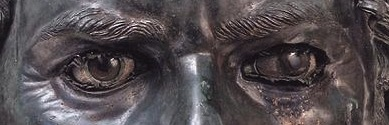
\includegraphics[scale=1]{graphics/seuthesiii.jpg}
	\caption{Detail of 4th century \textsc{bc} Thracian bronze portrait of King Seuthes \textsc{iii}}
	\label{fig:seuthesiii}
\end{figure}

If we suppose the eye to be an animal, perhaps it makes sense to think of the hypothetical creature as possessing the capacity to see. But if we relax that supposition, and consider an eye as it naturally occurs as part of an animal, then it would be wrong to think that an eye possesses the capacity to see. His eyes may have endowed King Seuthes III with the capacity to see, at least when he was alive, but they did not themselves possess this capacity. Similarly amputated eyes, eyes separated from the animal in which they naturally occur as parts, neither possesses the capacity to see nor endow anything else with that capacity. 

There are thus grounds for criticizing a commitment of Empedocles that arises in a passage that, as \citet[211]{Wright:1981zr} observes, Aristotle finds sufficiently interesting to quote three times (in \emph{De Anima} \textsc{iii}.6 430\( ^{a} \)27, \emph{De Caelo} \textsc{iii}.2 300\( ^{b} \)25, and \emph{De Generatione Animalium} \textsc{i}.18 722\( ^{b} \)17):
\begin{verse}
	as many heads without necks sprouted up\\
	and arms wandered naked, bereft of shoulders,\\
	and eyes roamed alone, impoverished of foreheads\\
	(Empedocles, DK \textsc{b}57; \citealt[64 245]{Inwood:2001ve})
\end{verse}
At a certain stage of the cosmic cycle, where Strife still dominates but whose influence is on the wane as Love grows stronger, the parts of animals arise spontaneously and in a disordered state. These combine to give rise to fantastical animals, some with clear mythological precedent:
\begin{verse}
	Many with two faces and two chests grew,\\
	oxlike with men's faces, and again their came up\\
	androids with ox-heads, mixed in one way from men\\
	and in another way in female form, outfitted with shadowy limbs.\\
	(Empedocles, DK \textsc{b}61; \citealt[66 247]{Inwood:2001ve})
\end{verse}
These animals tended not to survive. It is only when animal parts are combined in harmony, due to the increased influence of Aphrodite's Love, do the animals that we presently recognize emerge. Due to the harmony among their parts which fits them to a life in their natural environment, present animals not only survive but have the means of reproduction. Now consider the eyes roaming alone, impoverished of foreheads. Like amputated eyes, they are separated from animals in which they would harmoniously occur as parts. And like amputated eyes, they neither possess the capacity to see nor endow anything else with that capacity. Though eye-like in structure and composition, these are eyes in name only, at least by Aristotle's lights:
\begin{quote}
	What a thing is is always determined by its function: a thing really is itself when it can perform its function; an eye, for instance, when it can see. When a thing cannot do so it is that thing only in name, like a dead eye or one made of stone, just as a wooden saw is no more a saw than one in a picture. (\emph{Meterologica} \textsc{iv}.12 390\( ^{a} \)10--14; Webster in \citealt[86]{Barnes:1984uq})
\end{quote}

The capacity to cut in the manner of axes is a power and potentiality. A thing may possess this power, and so retain the potential to cut in that manner, even when at rest, when it is not actually cutting anything. Similarly, the capacity to see is a power and potentiality. A thing may possess or endow this power, and so retain the potential to see, even when at rest, when it is not actually seeing anything, because of darkness or sleep, say. Aristotle also claims that, in general, matter is potentiality and that form is actuality. There is no inconsistency here as the actual and the potential are said of in many ways. A thing is actually an axe if it possesses what it takes to be an axe, the capacity to cut in the manner of axes, the form and substance of an axe. Moreover the material parts of the thing, the matter of the axe---the wooden shaft, the bronze head---are potentially an axe since they are capable of taking on the form of an axe. When the bronze is suitably fashioned, and honed, and securely fixed to the wooden shaft, the matter, in taking on the form that it does, in so acquiring the capacity to cut in the manner of axes, realizes this potentiality. But what it is to be an actual axe is itself a power and potentiality, the capacity to cut in the manner of axes, a potentiality actualized in so cutting. Similarly, a thing is actually an eye if it possesses what it takes to be an eye, the capacity to see, the form and substance of an eye. Moreover the material parts of the thing, the matter of the eye---the membrane, the interior water---are potentially an eye since they are capable of taking on the form of an eye. When interior water is bound by the membrane and the other parts of the eye are suitably arranged, the matter in taking on the form that it does, in so acquiring the capacity for sight, actualizes this potentiality. What it is to be an actual eye is itself to possess or endow a power and potentiality, the capacity to see, a potentiality actualized in seeing.

The actual and the potential are said of in many ways. In his discussion of these analogies, Aristotle distinguishes two senses of the actual/potential distinction. There is an initial potentiality had by some matter. This potentiality is realized by that matter taking on a form. The taking on of the relevant form is the first actuality. However, in the cases at hand, the relevant form is understood as the possession, or perhaps the endowment of, a capacity. So the first actuality is itself a potentiality. The realization of this potentiality, the exercise of the capacity which is the form of the matter, is the second actuality. These distinctions are schematically represented in table~\ref{tab:potential}

\begin{table}[htbp]
	\centering
		\begin{tabular}{cccc}
			& \emph{An Axe} & \emph{An Eye}\\
			\hline
			\emph{Potenitality} & the matter of an axe & the matter of an eye\\
			\hline
			\emph{First Actuality} & the capacity to cut & the capacity to see\\
			\hline
			\emph{Second Actuality} & cutting & seeing\\
			\hline
		\end{tabular}
	\caption{Two senses of the actual/potential distinction}
	\label{tab:potential}
\end{table}

Eyes endow animals that possess them with the capacity to see. This is a capacity that animals enjoy even when asleep or inattentive. Endowing the perceiver with the capacity for sight is what the organ of sight is for. As \citet{Johansen:1997zr} argues, this further teleological claim motivates a certain explanatory strategy with respect to the anatomical structure of the eye, what he describes as a ``top-down explanation''. Begin with what the organ of sight is for, to endow its possessor with the capacity to see. If the perceiver is endowed with this capacity, then the primary objects of sight, the colors of remote external particulars, potentially appear in the perceiver's experience of them. In order for the colors of remote external particulars to appear in the perceiver's experience of them, the organ of sight must be transparent. Sight is a reactive capacity, the organ of sight must be acted upon for sight to be exercised. And color only ever acts, even mediately, upon what is actually transparent. The eye has the structure and composition that it does to sustain the transparency necessary to endow the perceiver with the capacity for sight. So our initial discussion of transparency (chapter~\ref{cha:transparency}) was necessary not only to understand Aristotle's definition of color (chapter~\ref{cha:color}) but also to understand Aristotle's explanatory strategy with respect to the anatomical structure of the eye. And understanding Aristotle's explanatory strategy, here, will yield insight into the significance of its limitations.



% section the_soul_of_the_eye (end)

\section{Transparency and the Anatomy of the Eye} % (fold)
\label{sec:transparency_and_the_anatomy_of_the_eye}

Why must the organ of sight be transparent?

Sight is a reactive capacity. It is a mode of sensitivity to the colors of remote external particulars. It only acts by reacting to the presence of a particular's color. Since sight is a reactive capacity, it must be acted upon in order for it to be exercised. That its exercise, an episode of seeing, just is being acted upon in this way is a further claim, that Aristotle denies, \emph{De Anima} \textsc{ii}.5. (For a contemporary defence of this denial see \citealt{Travis:2009fk} and \citealt{Kalderon:2012fk}.) Color could not immediately act upon the eye, since contact would blind the perceiver to the particular and its color. Contact precludes sensation, to be palpable is to be imperceptible. Nevertheless, the color of a remote external particular can act upon the eye mediately, by acting upon the intervening medium. Thus was the moral of Aristotle's criticism of Democritus and Empedocles (chapter~\ref{sec:against_the_empedoclean_principle}). The eye is itself affected by the color's effect on light. Since color is the power to alter what is actually transparent, the eye is affected by color's effect on transparent media by itself being transparent, at least in part. They eye is transparent, then, at least in part, so that the colors of remote external particulars may mediately act upon it. Which they must be capable of doing, since sight is a reactive capacity, a mode of sensitivity to the colors of remote external particulars arrayed in the natural environment.

Suppose that is right. Suppose that sight could only be the reactive capacity that it is, a chromatic sensitivity, if the organ of sight were transparent, at least in part. This would constrain its elemental composition. Whereas some elements are receptive to the presence and activity of the fiery substance, such as air and water, other elements, such as earth, exclude the fiery substance or at least retard its activity. Transparency is present only in matter with a certain elemental composition, one that allows for the presence and activity of the fiery substance.

That sight is a reactive capacity, a chromatic sensitivity, not only constrains the elemental composition of the eye, but it also constrains its structure. Transparency is a nature or power common to different substances such as water and air. So the requirement that the internal medium of the eye be transparent does not by itself determine whether an eye must have either elemental composition. Further material considerations determine that the internal medium be water:
\begin{quote}
	True, then, the visual organ proper is composed of water, yet vision appertains to it not because it is water, but because it is transparent---a property common alike to water and to air. But water is more easily confined and more easily condensed than air; it is that the pupil, i.e. the eye proper, consists of water. (\emph{De Sensu} \textsc{ii} 438\( ^{a} \)13--18)
\end{quote}
Air and water are liquids and so lack fixed boundaries. If the organ of sight is thus composed, at least in part, of the transparent, this liquid must somehow be confined to the organ of sight, by a fine membrane (like the membrane with which Aphrodite's Love enshrouds the primeval fire in the eye's interior, Empedocles DK 84). That this is more easily done with water than air favors the conclusion that the eye is composed, at least in part, of water. However, what is presently important is that reflection on the material constraints of sustaining an internal transparent medium not only determines the elemental composition of the internal medium but also significant anatomical structure, the existence of a membrane that confines and condenses the internal water.

That the eye is composed of water, at least in part, receives additional empirical support from gross anatomical observation. Water flows from decomposing eyes (\emph{De Sensu} \textsc{ii} 438\( ^{a} \)17), and this water is remarkably cold and glistening when it flows from the eyes of embryos (\emph{De Sensu} \textsc{ii} 438\( ^{a} \)18). Whereas in sanguineous animals, the eye contains fat and oil to prevent the water from freezing, the eyes of bloodless animals are covered for the the same reason (\emph{De Sensu} \textsc{ii} 438\( ^{a} \)20--3).


Aristotle's anatomy of the eye recapitulates important aspects of the ingestion model, as presented in the answer in the style of Gorgias (\emph{Meno} 76\( ^{a-d} \)):
\begin{quote}
	Now, as vision outwardly is impossible without light, so also it is impossible inwardly. There must, therefore, be some transparent medium within the eye, and, as this is not air, it must be water. The soul or its perceptive part is not situated at the external surface of the eye, but obviously somewhere within: whence the necessity of the interior of the eye being transparent, i.e. capable of admitting light. And that it is so is plain from actual occurrences. It is matter of experience that soldiers wounded in battle by a sword slash on the temple, so inflicted as to sever the passages of the eye, feel a sudden onset of darkness, as if a lamp had gone out; because what is called the pupil, i.e. the transparent, which is a sort of lamp, is then cut off. (\emph{De Sensu} 438b7-438b15)
\end{quote}
This passage is the culmination of a dialectic that began at \emph{De Sensu} 437\( ^{b} \)11. An explanation of vision in terms of the eye's fiery emission, attributed to Empedocles and Plato in the \emph{Timaeus}, is contrasted with the competing explanation of Democritus in terms of the eye's reflection. The passage presents a complex dialectical refinement of the \emph{endoxa}. The explanations of Empedocles and Democritus are, of course, rejected. Importantly, however, Aristotle retains elements of each of their explanations, even if these elements are fundamentally reconceived.

According to Aristotle, Democritus maintains that the eye sees because of its reflective surface, itself due to the smoothness of the eye and the presence of lachrymal fluid (\emph{De Sensu} 438\( ^{a} \)5--12). Democritus is wrong in thinking that this was due to water's capacity for reflection, and consequently wrong in taking the locus of sight to be on the surface of the eye. Nevertheless, Democritus was right to link the eye's capacity to see with the presence of water. However, it is not the reflectivity but the transparency of the eye's water that is required to endow its possessor with the capacity to see. 

% If Democritus was right in thinking that the eye is composed of water, then Empedocles was wrong in thinking that the eye contained fire. This should not obscure for us the way in which Aristotle retains important elements of the Empedoclean theory of vision.

This parallels the way that Empedocles accommodates the dominant medical opinion of his time (discussed in chapter~\ref{sec:empedocles_theory_of_vision}). The presence of lachrymal fluid is both necessary for sight and necessary for the reflective appearance of the eye. This encouraged the opinion that the reflective appearance of the eye explained the eye's receptivity to sight, and hence that the surface of the eye is the locus of sight. However, on the ingestion model, the assimilation of chromatic effluences is a material precondition for their presentation to the organ of sight. On the ingestion model, sight is located within. By conceiving of the receptors on the surface of the eye as water-bound passages to its interior, Empedocles reconciles the ingestion model with the dominant medical opinion of his time. Similarly, Aristotle asserts that ``the soul or its perceptive part is \ldots\ obviously within'' (\emph{De Sensu} \textsc{ii} 438\( ^{b} \)9--10). And like Empedocles, Aristotle retains something of Democritus opinion. But not by finding a role for the surface of the eye in seeing, but by claiming that the eye is partly composed of water. However, as we shall see, the transparent plays a role similar to the role played by ocular passages in Empedocles's theory of vision.

Aristotle rejects the explanation of vision in terms of the eye's fiery emission. While Aristotle attributes this view to Empedocles on the basis of the lantern analogy (DK 84; quoted in full at \emph{De Sensu} \textsc{ii} 437\( ^{b} \)27--438\( ^{a} \)3), he also writes:
\begin{quote}
	Sometimes he accounts for vision thus, but at other times he explains it by emanations from the visible objects. (\emph{De Sensu} \textsc{ii} 438\( ^{a} \)3--4)
\end{quote}
As discussed in chapter~\ref{sec:empedocles_theory_of_vision}, Aristotle thinks that Empedocles is potentially offering distinct explanations of color vision---one in terms of the eye's emission of fiery effluence and the other in terms of the eye's assimilation of chromatic effluences. While Aristotle rejects the explanation of color vision in terms of the eye's fiery emission, he reinterprets Empedocles' lantern analogy on the model of the answer in the style of Gorgias, though with crucial refinements.

While rejecting the explanation of vision in terms of the eye's fiery emission, nowhere does Aristotle directly deny the fundamental claim of Empedoclean a\-nat\-o\-my that the eye is composed of ``fire and its opposite'' (Theophrastus, \emph{De Sensibus}, \textsc{xv}). Perhaps, this is not an omission on Aristotle's part but intentional, for there is another way to understand Empedocles talk of interior fire. If the eye's interior is composed of confined and condensed water in order to sustain its transparency, then the interior water, being transparent, is receptive to the presence and activity of the fiery substance. The external medium must be illuminated if the color of a remote external particular is to be visible in it. Similarly, for that color to be visible, the external light must be extended within. The transparent water of the eye's interior must itself be illuminated. And the internal medium is only illuminated by the presence and activity of the fiery substance. While seeing the white of the sun may not involve the assimilation of fiery effluences as Empedocles maintained, nevertheless, if the white of the sun is visible to the perceiver, this is due, in part, to the presence and activity of the fiery substance in the eye's interior. This is why Aristotle makes the deliberate allusion to Empedocles' lantern analogy (DK 84). Like Empedocles, Aristotle compares the eye to a lantern. But not because the eye emits fire the way a lantern does. But because the interior of the eye must be illuminated, the way the interior of a lamp is illuminated, if the external scene is to be visible. So not only does Aristotle retain the phenomenological insight of Empedocles, that seeing is a mode of assimilation, ``the soul or its perceptive part'' within. But Aristotle also retains the Empedoclean doctrine that the exercise of the capacity for sight involves fire in the eye's interior, understood as the fiery substance illuminating the internal medium. 

Though Aristotle reinterprets Empedocles' lantern analogy on the model of the answer in the style of Gorgias, there are crucial refinements, as he rejects the theory of effluences. 

According to Empedocles, what is assimilated is a material particular, a chromatic effluence, conceived as a fine body, composed of fire or water, with a distinctive magnitude. On Aristotle's reinterpretation of the lantern analogy, what is assimilated is not a material particular, but the state of the external medium, a state sustained by the illuminating presence and activity of the fiery substance. The state of the internal medium need not be the same as the state of the external medium. Internal and external media may differ in their degree of transparency, and so dark eyes may be illuminated to a lesser degree than the surrounding air. Nevertheless, the state of illumination of the interior water is determined by the amount of fiery substance encountered in the external medium and the degree of transparency of the internal medium, the degree to which it is susceptible to the illuminating presence and activity of the fiery substance. 

Despite rejecting the theory of effluences, the transparency of interior water plays, for Aristotle, a function that ocular passages play in Empedocles' theory of vision. Chromatic effluences, because of their distinctive magnitudes, are commensurate with ocular passages. As such, they can travel through such passages and so be palpable to the organ of sight. While a state lacks location, and so cannot travel, the external light is extended within, in the sense in which it can, so that the color of remote external particulars may be present in visual consciousness. It is thanks to the illuminated state of the eye's interior that the perceiver is able to assimilate the chromatic form of distal particulars in the natural environment. As I argued in chapter~\ref{sec:the_answer_in_the_style_of_gorgias}, the assimilation of chromatic effluences by the organ of sight is not, by itself, the sensing of colors. The assimilation of chromatic effluences is at best a material precondition for their sensing. Similarly, admitting light into the interior of the organ of sight is not, by itself, the sensing of colors. Interior illumination is at best a material precondition for their sensing. Sensing is the presentation of the color to the perceptive part of the soul, not by being palpable, but by the assimilation of chromatic form, by the color of remote external particulars shaping visual consciousness. However the doctrine of the assimilation of sensible form is to be understood, interior illumination is a material precondition for sensing, so understood. That the interior illumination takes on a character that depends on derives from the character of the exterior illumination may make the colors of remote external particulars perceptually available, but the perceptually availability of the colors only involves the colors being potentially perceived, not their actual perception.  

% This is another aspect of the ingestion model that is preserved in Aristotle's dialectical refinement of Empedocles' theory.

The present understanding of Aristotle's deployment of the lantern analogy is further confirmed by the empirical evidence that Aristotle marshals at the end of this passage (\emph{De Sensu} 438b12-15). That the eye must be ``capable of admitting light \ldots\ is plain from actual occurrences'', such as the blindness resulting from a wound sustained by a slash on the temple. Such a wound severs passages leading away from the eye and so impairs the eye's capacity to endow its possessor with sight. Though the wounded soldier's eyes are filled with light, since the passages leading within (presumably, to a position at or near the heart) are severed, the colors of remote external particulars are no longer present in his visual consciousness. While they appear through the internal medium, being actually transparent, the colors of distal particulars are cut off from the perceptive part of the soul. The wounded soldier can no longer assimilate the chromatic form of remote material particulars.

We have here another significant part of the eye's anatomy, the passages from the eye leading within. One should not anachronistically assume that Aristotle has in mind the optic nerve. Given that the seat of sensation is at or near the heart, a better hypothesis would be that they are vessels leading to the heart. However, Aristotle's description of these passages underdetermines any such identification \citep[see][]{Lloyd:1978fk}. In fact, Aristotle seems only interested in this anatomical detail insofar as these passages extends the transparent within. In extending the transparent within, the perceptive part of the soul becomes receptive to the direction of influence of the fiery substance. It is the presence and activity of the fiery substance that determines the sensible character of internal and external media. Moreover, the sensible character of transparent media is itself determined by the colors of the particulars that appear through that media. The precise content of the Aristotelian doctrine of the assimilation of sensible form remains, at this point, unclear. What is clear is that, first, it does not involve chromatic forms traveling in the manner of effluences, as \citet[\textsc{i} 1]{Hobbes:1651fk} imagined, and that second, the passages extending the eye's transparency within are necessary for the assimilation of chromatic form. 

Not only does Aristotle's empirical example provide us with another significant part of the eye's anatomy, but it also further illustrates what \citet{Johansen:1997zr} describes as Aristotle's ``top-down explanation''. Sight is the soul of the eye, or it would be if it were an animal. Endowing its possessor with the capacity for sight is what the organ of sight is for. Consequently the organ of sight is understood to have the structure and composition required to endow this capacity. Evidently, passages extending the transparent within are necessary for the capacity for sight, since when they are severed, the victims of such wounds are blinded. We have an explanation from what the organ of sight is for---to endow the perceiver with the capacity for sight---to anatomically significant structure---passages leading away from the eye.

So far we have distinguished the condensed and confined water in the eye's interior, the membrane that confines it, the pupil, and passages leading away from the eye to some point in the interior, perhaps, at or near the heart. In addition, Aristotle distinguishes the dark of the eye from the light (\emph{De Sensu} \textsc{ii} 437\( ^{b} \)1), understood as the iris and the white of the eye that surrounds the iris (\citealt[see][218, 231 n13]{Lloyd:1978fk}). In sanguineous animals, the white is fat and oily to prevent the transparent water of the eye from freezing (\emph{De Sensu} \textsc{ii} 438\( ^{a} \)20--3). The contrast must be with the dark of the eye, as opposed to the black, since Aristotle recognizes different colored irises: ``In some it is black, in some distinctly blue, in some greyish-blue, in some greenish'' (\emph{Historia Animalium} \textsc{i}.10 492\( ^{a} \)2--3). Blue, grayish-blue, and greenish may be dark, at least when compared with the white of the eye, but they are not black. Further evidence, if any were needed, that \emph{melaton} and its cognates should be understood as dark as opposed to black in the Aristotelian color scheme.

The Aristotelian anatomy of the eye is crude, even by ancient standards. Lloyd summarizes its limitations:
\begin{quote}
	Yet no attempt is made to describe the structure of the eye as a whole, although this is, of course, complex. The three main parts Aristotle identifies quite incidentally in the course of this chapter, pupil, iris, white, relate primarily to the superficial appearance of the eye. Apart from the one reference to the membrane of the eye and the one reference to certain \emph{poroi}, already mentioned, his remarks on the internal structure of the eye are confined to the point that the pupil, \emph{kore}, consists of water. We may take it that this refers to the vitreous humour that occupies most of the bulb of the eye and which, in certain lesions, might produce a watery discharge. But there is no mention of the membrane enveloping the vitreous humour (retina, choroid, sclera), nor of the lens, nor of the anterior chamber between the cornea and the lens. There is, in fact, no mention of most of the parts that seem difficult to identify straightforwardly as water, and no systematic description of the internal structure of the eye as such at all. \citep[220--221]{Lloyd:1978fk}
\end{quote}
While the Aristotelian anatomy of the eye can be further refined and extended (and was by the commentators---Philoponus recognized the anterior chamber between the cor\-nea and the lens), important limitations will inevitably remain. The significance of these limitations should be judged in relation to the specific explanatory concerns Aristotle and the Peripatetic tradition were addressing in articulating the eye's anatomy. \citet{Lloyd:1978fk} takes Aristotle to be primarily addressing the problem of how to assign the four elements to the five senses. This is indeed a task of \emph{De Sensu}. But as I have argued, Aristotle has more specific explanatory concerns. The eye must have such a nature so as it may be mediately acted upon by color in order to endow its possessor with the reactive capacity for sight. Taken by itself, this claim is the expression of a reasonable explanatory strategy. If Aristotle's anatomy of the eye strikes us as superficial or schematic, this is not due to this explanatory strategy alone, nor is it due to an abstract taxonomic concern with assigning elements to senses. Rather, two further claims are responsible for the limitations of Aristotelian anatomy: (1) that the eye can only be mediately acted upon if it is actually transparent, and (2) that the eye is only acted upon by altering the character of its interior illumination. Whereas (1) specifies a condition on the patient of change, (2) specifies the nature of the change. It is these further commitments that lead him to discern only those parts of the eye that might plausibly be said to play a role in sustaining the transparency of the internal medium.


% section transparency_and_the_anatomy_of_the_eye (end)

\section{Interior Illumination} % (fold)
\label{sec:interior_illumination}

The eye in seeing is like a lantern, not because it emits fire from its interior, but because in seeing the interior of the eye is illuminated. The confined and condensed water in the interior of the eye is transparent for the sake of receiving such illumination. It is only be being transparent that colors can mediately act upon the eye by acting upon the intervening medium. And since sight is a reactive capacity, a mode of chromatic sensitivity, the organ of sight must be acted upon if the capacity for sight is to be exercised in seeing the presented color.

What is the effect that the color produces in mediately acting upon the eye?

Since color acts upon the eye by acting upon the external me\-di\-um, the effect on the internal medium should be of the same kind as the effect that color has on the external medium. Aristotle explicitly speaks of admitting light. Colors affect the character of the illuminated medium, so in admitting light, the transparent medium within the eye not only must be actually transparent, due to the illuminating presence and activity of the fiery substance, but it must also come to have a character that at least corresponds to the character of the external illuminated medium. The correspondence need not be identity. As we observed, internal and external media may differ in their degree of transparency, and so dark eyes may be illuminated to a lesser degree than the surrounding air. The light admitted by dark eyes, their interior illumination, will not be as bright as the exterior illumination. Nevertheless, the existence and character of the interior illumination depends upon and derives from the existence and character of the external illumination that immediately acts upon it.

This places an important metaphysical constraint on the character of the interior illumination. Whatever effect color has on the external medium, such as the surrounding air, the external medium has a corresponding effect on the internal medium. In chapter~\ref{sec:the_definition_of_color}, we reviewed some candidate effects. Given the metaphysical constraint, the candidate effects on the internal medium, the illuminated water in the eye's interior, correspond to these.

In chapter~\ref{sec:the_definition_of_color}, I argued that color could not color external media since doing so would be inconsistent with the way that colors are perceptually available within them---either by being inconsistent with the medium being actually transparent or by being inconsistent with the directionality of the visible. The agent of a change must actually be the way that the patient potentially is. Insofar as the external medium acts upon the internal medium---light is admitted---the external medium is an agent of change, the internal medium the patient. Since the external medium could not be colored, in admitting light, the internal medium, the transparent water within the eye's interior, could not in turn be colored. This result is one of the advantages of the present mode of exposition, focused fundamentally on the nature of the transparent, that begins with color's effect on external transparent media before considering color's mediate effect on internal transparent media.

As before, three candidate effects remain:
\begin{enumerate}[(1)]
	\item The rendering visible of the transparent---making the transparent internal me\-di\-um perceptually available
	\item The rendering visible of colored particulars arrayed in the transparent external me\-di\-um\----making the colored particulars perceptually available
	\item Affecting the fiery substance by affecting the amount of it in the internal me\-di\-um, the water within the eye, or, if this does not come to the same thing, promoting or retarding its activity to some degree, or otherwise affecting its direction of influence
\end{enumerate}
(1) follows from the \emph{De Anima} (\textsc{ii}.7 418\( ^{b} \)4--6) definition of the transparent. It might seem odd to claim that the transparent water in the eye's interior is perceptually available to us, even when illuminated. However, recall, by Aristotle's definition of transparency, the transparent appears to us by the colors of remote external particulars appearing through it. Since when we see the colors of remote external particulars, we see them through the transparent medium in the eye's illuminated interior, we see that medium as well. Of course, ordinarily we do not attend to the transparency of the eye's interior water until it is disrupted, when we see floaters, say. But, in seeing the colors, the internal medium must itself be perceptually available, at least in the manner of transparent things enshrined in the \emph{De Anima} definition of transparency. (2) is not only a consequence of the \emph{De Anima} definition, but is a commitment of Aristotle's description of the wounded soldier. That the colored particulars arrayed within the transparent external medium are perceptually available within the water in the eye's interior is demonstrated by severing the illuminated interior from the perceptive part of the soul, located at or near heart. When the transparency in the eye's interior is no longer extended within, the passages leading from the eye having been severed by a sword's blow, the colors of remote external particulars are no longer perceptually available. The soldier has been blinded by his wound. (3) not only draws upon materials available in both \emph{De Anima} and \emph{De Sensu}, but coheres well with the \emph{De Sensu} project of explaining what each of the sense object must be to produce the sensation in full actuality. (1) and (2) are psychological effects in that perceptual availability is or involves potential perception. (3) is not psychological, even in this extended sense, but is, rather, a material change. These psychological and material changes need not be inconsistent. They may be part of formal and material explanations of the same phenomena. 

Given the proportion of the transparent that exists in all bodies, colored particulars have the power to affect the amount, activity, and direction of influence of the fiery substance in illuminated media. In so affecting the fiery substance, the particular, or at least its color, is perceptually available. In acquiring the power to affect light in a certain way, the colored particular also acquires the power to mediately affect the eye, the organ of sensation sensitive to such alterations in illuminated media. When the transparent water in the eye's interior is suitably aligned to the direction of influence of the fiery substance illuminating the external medium, interior water is immediately illuminated, 

% If color vision is a mode of sensitivity to the chromatic form of remote external particulars, the organ of sight must be acted upon

% section interior_illumination (end)

% chapter the_eye (end)

%!TEX root = /Users/markelikalderon/Documents/Git/formwithoutmatter/aristotle.tex
\chapter{Two Transitions to Actuality} % (fold)
\label{cha:two_kinds_of_potentiality}

\section{The Problem} % (fold)
\label{sec:the_problem}

The eyes, in seeing, are altered. They are filled with light. The existence and character of the interior illumination depends upon and derives from the existence and character of exterior illumination, itself affected by the colors of remote external particulars. Moreover, the eyes in seeing must be altered. The eyes are the organ of sight, and seeing is a reactive capacity. Sight only acts by reacting to the colors of remote external particulars. So the organ of sight must be acted upon in order to exercise the capacity for sight. Notoriously, however, Aristotle denies that the exercise of our capacity for sight, an episode of seeing, is itself an alteration. So the eyes, in seeing, must be altered, but seeing is not itself an alteration or, at least, it is not an alteration of the usual sort. What kind of change does a perceiver undergo when seeing? 

The avowed task of \emph{De Anima} \textsc{ii} 5 is to say, in a preliminary fashion, what the senses are in general. A discussion of the special senses follows in subsequent chapters, and it is only in \emph{De Anima} \textsc{ii} 12 that Aristotle give the official definition of perception as the assimilation of sensible form without the matter of the perceived particular. Despite the avowed task of the chapter, most of the discussion is bound up with a number of careful distinctions, and we only get the general characterization of sensation at the end of the chapter. 

% section the_problem (end)

\section{The \emph{Endoxa}} % (fold)
\label{sec:the_endoxa}

The chapter begins with a discussion of the \emph{endoxa}:
\begin{quote}
	Sensation depends, as we have said, on a process of movement or affection from without, for it is held to be some sort of change of quality. Now some thinkers assert that like is affected only by like. In what sense this is possible and in what sense impossible, we have explained in our general discussion of acting and being acted upon. (Aristotle, \emph{De Anima} \textsc{ii} 5 416\( ^{b} \)33--417\( ^{a} \)2; Smith in \citealt[29]{Barnes:1984uq})
\end{quote}
Aristotle is picking up on his previous discussion of the \emph{endoxa} from \emph{De Anima} \textsc{i} 5 410\( ^{a} \)24--410\( ^{b} \)14. That perception depends upon being moved and acted upon was attributed to previous thinkers in \emph{De Anima} \textsc{i} 5 410\( ^{a} \)25--26. That claim, at least in the present context, is importantly qualified. Perception is not identified with being moved and acted upon. It is only said to depend upon being moved and acted upon. Though perhaps a widely held opinion, not all previous thinkers assented to it. Notoriously, in the Secret Doctrine that Socrates attributes to Protagoras (\emph{Theaetetus} 156\( ^{a-c} \)), perception is represented as the outcome of active and passive forces in conflict and so no mere passive effect. And this is perhaps echoed in Plato's own account of perception as the outcome of emanations from the perceiver and the object perceived coalescing (\emph{Timaeus} 45\( ^{b} \)--46\( ^{a} \)). In an earlier chapter, Aristotle suggested that perception was a qualitative alteration (\emph{De Anima} \textsc{ii} 4 415\( ^{b} \)24). That claim reappears though again in qualified form. Smith translates the qualification as ``some sort of change of quality'', but as \citet[36--37]{Burnyeat:2002an} importantly points out, the qualification can also be understood as ``a change of quality of a sort'', that is, as an alteration only in an etiolated sense. In the first line of the passage the claim that perception is a sort of alteration, or alteration of a sort, is offered as a justification for thinking that perception is a way of being moved and acted upon. That justification draws, implicitly, upon Aristotle's physics. In \emph{Physica} \textsc{vii} 1 and \textsc{viii} 4, Aristotle argues that every case of motion involves being acted upon, and in \emph{De Generatione et Corruptione} \textsc{i} 6 323\( ^{a} \)13--24 he argues that alteration always involves being acted upon. The attribution of the claim that perception is some sort of alteration, or alteration of a sort, to previous thinkers is doubtful, however, as it makes essential use of the classificatory scheme of the \emph{Categoriae}. Here, as is not uncommon, Aristotle is endeavoring to understand the views of his predecessors in his own terms. Aristotle may be over-reading, or having dialectical rather than strictly historical concerns, but, to be fair, the connection with qualitative alteration is not far to seek insofar as previous thinkers maintained, as well, that like is affected only by like.

The like-by-like principle, that like is affected only by like, is more genuinely of pre-Aristotelian provenance. Empedocles, among others, is said to have held it (\emph{De Anima} \textsc{i} 2 404\( ^{b} \)7--15; though whether he actually held the like-by-like principle is controversial, see \citealt{Kamtekar:2009fk}). Concerning ``in what sense this is possible and in what sense impossible'', Aristotle refers us to \emph{De Generation et Corruptione} \textsc{i} 7 (on Aristotle's use of cross-referencing in this chapter see \citealt{Burnyeat:2002an}). There, Aristotle explains that there is a sense in which those who maintain that like is affected by like and those who maintain, instead, that like is unaffected by like are both right. Each position, though seemingly contradictory, capture part of a more complex truth (\emph{De Generatione et Corruptione} \textsc{1} 7 323\( ^{b} \)15--324\( ^{a} \)9). Consider the case of one thing acting upon another thus inducing a change of quality, say, fire heating a pot of cool water. (My choice of example, though drawn from \emph{De Generatione et Corruptione}, is far from innocent---in \emph{De Anima} \textsc{ii} 12 Aristotle will contrast a plant being warmed with an animal's sensation of heat.) At the start of the process, the agent and patient of the change, the fire and the water, have contrary qualities from the same range of qualities---the fire is hot and the water is cool and each is a quality of temperature. They are thus generically alike. Though they are generically alike prior to the alteration they are also unlike. The distinct qualities they possess from the same range are contraries. They need not be opposites, qualities at the extreme ends of an ordered range of qualities, they may be intermediate qualities from the same range, so long as they are contraries. Thus the fire and the water, while generically alike in being the kinds of thing that have temperature, are specifically unlike in possessing contrary qualities of temperature. When the fire comes into contact with the pot of water they interact in such a way that the water becomes hot and so like the way the fire was prior to the qualitative alteration. So the water was initially unlike the fire that heated it in being cool but became like that fire in becoming hot. 

In \emph{De Generatione et Corruptione} Aristotle argues against the like-by-like principle as follows:
\begin{quote}
	Moreover, if like can be affected by like, a thing can also be affected by itself; and yet if that were so---if like tended in fact to act \emph{qua} like---there would be nothing indestructible or immovable, for everything would move itself. (Aristotle, \emph{De Generatione et Corruptione} \textsc{i} 7 323\( ^{b} \)21--23; Joachim in \citealt[23]{Barnes:1984uq})
\end{quote}
A variant of this argument occurs at this point in \emph{De Anima} \textsc{ii} 5 (discussed earlier in chapter~\ref{sub:particular}): 
\begin{quote}
	Here arises a problem: why do we not perceive the senses themselves, or why without the stimulation of external objects do they not produce sensation, seeing that they contain in themselves fire, earth, and all the other elements, of which---either in themselves or in respect of their incidental attributes---there is perception? It is clear that what is sensitive is so only potentially, not actually. The power of sense is parallel to what is combustible, for that never ignites itself spontaneously, but requires an agent which has the power of starting ignition; otherwise it could have set itself on fire, and would not have needed actual fire to set it ablaze. (Aristotle, \emph{De Anima} \textsc{ii} 5 417\( ^{a} \)3--9; Smith in \citealt[29]{Barnes:1984uq})
\end{quote}
If the like-by-like principle were true, then the sense organ, being like itself---as, indeed, is everything else---would act upon itself. The exercise of the capacity for sight, which the eye endows its possessor with, would not require an external particular to activate it. However, as \citet[226--227]{Polansky:2007ly} observes, the argument, when restricted in this way to perception, accrues new significance. If the sense organ acts upon itself, then the exercise of the capacity it endows its possessor with would at best be a mode of self-consciousness. It would not be a mode of sensitivity to external particulars and their sensible qualities and thus could not be a mode of perception. The puzzle, as it arises in the context of \emph{De Anima} \textsc{ii} 5, thus concerns the very possibility of perception.

The puzzle about the like-by-like principle in the perceptual case is epistemically significant since it concerns the very possibility of perception. Perception must be a reactive capacity, if it is to be perception at all, otherwise it would not be a mode of sensitivity to remote external particulars arrayed in the natural environment. However, being a reactive capacity is merely a necessary condition for perception. The objectivity of perceptual content depends not only upon perception only ever acting by reacting to the presence of external particulars but also on the perceiver, or perhaps their perceptual experience, becoming like those external particulars actually are. Sheer receptivity is insufficient for sensory presentation. It requires, as well, the assimilation of the sensory object.

Not only does the puzzle about the like-by-like principle accrue new significance in \emph{De Anima} \textsc{ii} 5, but it is susceptible to a novel solution as well. Nowhere in \emph{De Generatione et Corruptione} \textsc{i} 7 does Aristotle explicitly appeal to the distinction between the actual and the potential. But that distinction is essential to the present resolution of the puzzle. The lesson of the puzzle about perception raised by the like-by-like principle is that the capacity for sight, the form and substance of the eye, is a kind of potentiality, one that requires an external particular, the object of perception, to act upon the eye in order for that capacity to be exercised in seeing that object. It is like fuel which requires an external fire for it to ignite. Perception, as we have seen, is essentially a reactive capacity, one which requires an external object to ignite sensory consciousness.

Perception is a power or potentiality that requires an external particular for it to be realized. The exercise of perceptual capacities is, at least in this regard, like the case of motion, studied in \emph{Physica}, since all motion requires a mover:
\begin{quote}
	To begin with let us speak as if there were no difference between being moved or affected, and being active, for movement is a kind of activity---an imperfect kind, as has elsewhere been explained. Everything that is acted upon or moved is acted upon by an agent which is actually at work. Hence it is that in one sense, as has already been stated, what acts and what is acted upon are like, in another unlike; for the unlike is affected, and when it has been affected it is like. (Aristotle, \emph{De Anima} \textsc{ii} 5 417\( ^{a} \)15--21; Smith in \citealt[30]{Barnes:1984uq})
\end{quote}
Aristotle invites us to speak as if being moved and acted upon, on the one hand, and perceptual activity such as seeing and hearing, on the other, were the same. He is not identifying perception with being moved or acted upon, but merely emphasizing the fact that, like the motion of natural bodies discussed in \emph{Physica}, the activity of the senses depends upon an external cause---the external particular mediately acting upon the organ of sensation.

In \emph{Physica} \textsc{iii} 1 201\( ^{a} \)10--11, Aristotle defines motion as the actuality of the potential as such (see also \emph{Metaphysica} \textsc{k} 9 1065\( ^{b} \)16). Against Parmenidean skepticism, Aristotle insists upon the reality of change. Becoming pertains to actuality, but, in a concession to Parmenidean skepticism, it does so in a qualified manner. Consider again our example of qualitative alteration, fire heating a pot of cool water. At the beginning of this process, the water is cool but potentially hot. At the end of this process, the water is no longer potentially but actually hot. When the process has finished and the water is actually hot, the water is no longer becoming hot. It is this transition from merely being potentially hot, possessed by the water prior to its contact with the heat of the flame, to being actually hot which is the motion of qualitative alteration. This is something that actually happens, hence the use of actuality in Aristotle's definition of motion. But throughout the process, until its termination, the water remains potentially hot. That is why motion is the actuality of the potential as such. When the water is actually hot it is no longer potentially hot. The alteration that the water undergoes is the actualization of its potentially being hot, a potentiality that is both realized and exhausted in the process. (That the relevant sense of potentiality is potential for being rather than changing see \citealt{Kosman:1969aa}; though see \citealt{Heinaman:1994aa} for criticism.)

We are now in a position to understand the sense in which the motion involved in qualitative alteration is imperfect or incomplete. It is incomplete in the sense that when the terminal state has been reached, the process of alteration is no longer happening, and so long as it is happening, the terminal state has not been reached. The incompleteness of motion is linguistically manifest in our inability to simultaneously use present and perfect tenses to describe that motion. Having built a house, the builder is no longer building. And so long as the builder is building the house has yet to have been built (\emph{Metaphysica} \( \Theta \) 6 1048\( ^{b} \)18--34). This would contrast with an activity whose end lies not without but is immanent in the activity itself. Aristotle marks such a contrast at the opening of the \emph{Ethica Nicomachea} \textsc{i} 1 1094\( ^{a} \)3--5, and there is an extended discussion in \emph{Metaphysica} \( \Theta \). Aristotle does not explicitly describe these activities as complete. However, if we follow the post-Aristotelian vocabulary, then complete activity, activity whose end is immanent in the activity itself, is linguistically manifest in the simultaneous availability of the present and perfect tenses in describing that activity. One sees the sun and has seen it. One is enjoying and has enjoyed. The intelligibility of conjoining the present and perfect tenses indicates that the described activity is an end in itself, in contrast to the case of motion which is always progress towards an end that lies without.

At the end of the passage, Aristotle offers a resolution of the apparent conflict between those who maintain that like affects like and those who maintain that like is unaffected by like that echoes the resolution offered in \emph{De Generatione et Corruptione} \textsc{i} 7. There is a sense in which both opinions are correct. The water, at the beginning of the process, is cool and so unlike the heat of the flame. But when the process is completed and the water's potential for being hot is realized, the water is like the way the fire was prior to the alteration. 

We have seen how perceptual activity is like qualitative alteration in that it requires an external object to act upon the sense organ to initiate that activity. The present resolution of the apparent conflict in the \emph{endoxa} hints at a further analogy. Applying it to the case of perception yields the following result. Prior to seeing the brilliant white of the sun, the perceiver, or perhaps their perceptual experience, is unlike the sun. But in coming to see the sun's brilliant whiteness, the perceiver, or perhaps their perceptual experience, becomes like the way the sun was prior to seeing it. The perceiver, or their perceptual experience, is potentially like the sensible object, and when they undergo the perceptual experience of that sensible object their experience becomes actually like the way the sensible object was prior to perception. We have here an anticipation of the general characterization of perception that occurs at the end of \emph{De Anima} \textsc{ii} 5 and the definition of perception that occurs in \emph{De Anima} \textsc{ii} 12.

Aristotle's discussion of the \emph{endoxa} provides insight into how he is understanding assimilation as it figures in his definition of perception. In cases of qualitative alteration, at the end of the process, the patient assimilates the qualitative character of the agent of that change. The assimilation, here, is no material assimilation. Contrast the Empedoclean story of the movement of effluences through passages. That is straightforwardly a case of material assimilation---a material body, an effluence, is received within another body through a fine passage. In the case of qualitative alteration, as Aristotle understands it, nothing material is assimilated. What is assimilated is not a body, but a quality or state. And as I have observed in chapter~\ref{sec:transparency_in_de_anima}, whereas bodies have locations, qualities and states do not. We have here an important first step towards the resolution of Empedoclean puzzlement. Perceptual activity may not be an instance of qualitative alteration. Nevertheless, as in the case of alteration, the perceiver, or perhaps their experience, becomes like the way the perceived object was prior to perception. The perceiver, or their experience, assimilates the sensible object in a manner necessarily distinct from the material assimilation of that object, since to be palpable is to be imperceptible.

% section the_endoxa (end)

\section{Distinctions and Refinements} % (fold)
\label{sec:distinctions_and_refinements}

But we are getting ahead of ourselves. Before Aristotle offers the general characterization of perception, he undertakes to investigate the sense of potentiality involved in being a perceiver. Is the realization of this potential incomplete, in the way that alteration is? Or is the end of sight immanent in seeing? If the latter, then this would explain why perception is alteration of a sort, in an etiolated sense only. For while there would be significant analogies between qualitative alteration and perception---each involves an external cause and the assimilation of sensible form---if perceptual activity were complete, then it would not be a mode of alteration, even if it requires that the organ of sensation be acted upon to elicit that activity.

% section distinctions_and_refinements (end)

\subsection{The Triple Scheme} % (fold)
\label{sub:the_triple_scheme}

As we have had occasion to remark, according to Aristotle, the actual and the potential are said of in many ways. In \emph{De Anima} \textsc{ii} 5 Aristotle distinguishes two senses of potentiality, and correspondingly, two senses of actuality. The distinction occurs earlier in \emph{De Anima} \textsc{ii} 1 412\( ^{a} \)24--26 and occurs as well in \emph{Physica} \textsc{viii} 4 255\( ^{a} \)30ff. However, in \emph{De Anima} \textsc{ii} 1 the emphasis is on the two corresponding senses of actuality whereas in \emph{De Anima} \textsc{ii} 5 the emphasis is instead on possibility. The reason for this shift of emphasis is that in \emph{De Anima} \textsc{ii} 5 Aristotle's real concern is with the nature of the transition to actuality in each case, that is, with the nature of the change involved. Given that Aristotle understands motion in terms of potentiality in \emph{Physica}, it is natural for him to distinguish the relevant senses of potentiality and then distinguish the motions that correspond to these.

In \emph{De Anima} \textsc{ii} 5 the distinction is explained in terms of knowledge:
\begin{quote}
	But we must now distinguish different senses in which things can be said to be potential or actual; at the moment we are speaking as if each of these phrases had only one sense. We can speak of something as a knower either as when we say that man is a knower, meaning that man falls within the class of beings that know or have knowledge, or as when we are speaking of a man who possesses a knowledge of grammar; each of these has a potentiality, but not in the same way: the one because his kind or matter is such and such, the other because he can reflect when he wants to, if nothing external prevents him. And there is the man who is already reflecting---he is a knower in actuality and in the most proper sense is knowing, e.g. this A. Both the former are potential knowers, who realize their respective potentialities, the one by change of quality, i.e. repeated transitions from one state to its opposite under instruction, the other in another way by the transition from the inactive possession of sense or grammar to their active exercise. (Aristotle, \emph{De Anima} \textsc{ii} 5 417\( ^{a} \)22--417\( ^{b} \)1; Smith in \citealt[30]{Barnes:1984uq})
\end{quote}

In the passage, Aristotle contrasts someone ignorant of some subject matter but educable with a learned person knowledgeable about that subject matter. The ignorant but educable person is a knower in the sense that they potentially know something. They do not, for example, know some particular point of grammar, but it is not beyond their ken, and they can be brought to know it through education. Being composed of the right matter, they have the capacity for knowledge. The learned person is a knower as well. They have mastered the relevant point of grammar and, having mastered it, can be said to know it in the way that the ignorant but educable cannot. And Aristotle maintains that this sense of being a knower is also a kind of potentiality. Specifically, to know something is to have the capacity to apply that knowledge in a reasonable manner given the practical circumstances. Thus to apply the grammatical knowledge is to deploy it in one's speech or writing or to recognize its significance in the speech or writing of others, by recognizing a letter as an alpha, say. In exercising their knowledge, they can be said to know as well but in a different sense from one who possesses this knowledge without exercising it. To possess grammatical knowledge, in the relevant sense, just is to have the potential to exercise that knowledge in a reasonable manner given the practical circumstances. But this is a distinct sense of potentiality than is involved in the ignorant but educable's potentially knowing that point of grammar.  In the traditional, post-Aristotelian vocabulary, Aristotle is distinguishing between first and second potentiality and, correspondingly, between first and second actuality (schematically represented in table~\ref{tab:triple}). The vocabulary is post-Aristotelian since while Aristotle does speak of first actuality he does not generalize the vocabulary in the obvious way.

\begin{table}[htbp]
	\footnotesize
	\centering
		\begin{tabular}{ccc}
			\hline
			\emph{First Potentiality} & the capacity for knowledge & ``is a knower''\\
			\hline
			\emph{First Actuality/Second Potentiality} & knowing something & ``is a knower'', ``knows''\\
			\hline
			\emph{Second Actuality} & exercising that knowledge & ``knows''\\
			\hline
		\end{tabular}
	\caption{The triple scheme}
	\label{tab:triple}
\end{table}

The ignorant but educable is a knower in that they potentially know something. This is the first potentiality. In coming to know something this potentiality is realized. In coming to know something they too are a knower, though in a different sense. This is the first actuality. The first actuality of knowledge is itself a kind of potentiality since in knowing something the knower has the power or potentiality to exercise that knowledge in a reasonable manner given the practical circumstances. So, in the case at hand, the first actuality is also a second potentiality. In exercising that knowledge, in applying it in a reasonable manner given the practical circumstances, this potentiality is realized. This is the second actuality. 

At the end of the passage, Aristotle draws our attention to a corresponding difference in the two transitions to actuality. The transition from first potentiality to first actuality is a form of qualitative alteration in the way that the transition from second potentiality to second actuality is not. Instead of being a change of quality, the transition to second actuality is described as a transition from an inactive potentiality to its active exercise.

Describing learning as qualitative alteration can sound odd to modern ears. In assessing the credibility of this claim we should bear two things in mind. First, for Aristotle, the fundamental explanatory properties---the primary opposites, Hot and Cold, Dry and Wet---are sensible qualities. It should be no surprise, then, that coming to know should be understood by him in terms of qualitative alteration. That may help us, to some degree, understand why Aristotle found this claim more natural than we perhaps do, but moderns may still protest incredulity. However, knowledge, even on a modern conception of it, is a state. In coming to know about some subject matter, a person while initially in a state of ignorance about that subject is no longer ignorant but knowledgeable. But the replacement of one state by another inconsistent with it might fairly be described as a case of alteration.

How might these distinctions apply to the case of perception? Seeing is the exercise of an animal's capacity for sight. An animal's capacity for sight is a power or potentiality. It need not be exercised---say, when the animal is asleep or in the dark (at least in the case of seeing color if not the fiery or shining, see chapter~\ref{sec:the_objects_of_perception}). It is natural, then, to understand second potentiality as the animal's possession of a perceptual capacity and second actuality as its exercise. Indeed, at the end of the passage, Aristotle makes this connection explicitly. It is both the inactive potential for knowledge and sense to their active exercise which is the transition to second actuality (\emph{De Anima} \textsc{ii} 5 417\( ^{b} \)1; see also \emph{De Anima} \textsc{ii} 5 417\( ^{b} \)19). In which case, the second potentiality of perception, the possession of a perceptual capacity, is also the first actuality (\emph{De Anima} \textsc{ii} 5 417\( ^{b} \)17--19). 
% This is schematically represented in 
% 
% \begin{table}[htbp]
% 	\centering
% 		\begin{tabular}{ccc}
% 			\hline
% 			\emph{First Potentiality} & the matter of an animal & ``is a perceiver''\\
% 			\hline
% 			\emph{Second Potentiality/First Actuality} & the capacity for perception & ``is a perceiver'', ``perceives''\\
% 			\hline
% 			\emph{Second Actuality} & exercising that perceptual capacity & ``perceives''\\
% 			\hline
% 		\end{tabular}
% 	\caption{The triple scheme}
% 	\label{tab:triple}
% \end{table}

Here, however, we encounter a certain awkwardness. Coming to possess a perceptual capacity just does not seem analogous to learning a point of grammar. Indeed, insofar as animals are animate natural beings with perception---that is what distinguishes them from plants---as soon as an animal comes to be, it is endowed with perceptual capacities. So endowing a natural being with the capacity for perception seems more like generation than alteration. This is substantiated later in the chapter when Aristotle writes:
\begin{quote}
	In the case of what is to possess sense, the first transition is due to the action of the male parent and takes place before birth so that at birth the living thing is, in respect of sensation, at the stage which corresponds to the possession of knowledge. (Aristotle, \emph{De Anima} \textsc{ii} 5 417\( ^{b} \)17--19; Smith in \citealt[31]{Barnes:1984uq})
\end{quote}
There remains, however, an important point of analogy. Recall, Aristotle's curious remark that the ignorant but educable has the capacity for knowledge because of their matter. On the hylomorphic theory, matter is a kind of potentiality, and form is a kind of actuality. As we have seen (chapter~\ref{sec:the_soul_of_the_eye}), the form of the eye, its actuality, is its capacity to see. And the matter of the eye---the internal water, the membrane---is the potential to have that capacity. In the epistemic and perceptual cases, then, first potentiality is associated with the potentiality of matter. 

In the epistemic and perceptual cases, the transition to first actuality involves the actualization of the potentiality of matter. Even if a certain awkwardness remains, there is a sense in which the strength of the analogy does not matter. In the perceptual case, Aristotle's real focus is on the transition to second actuality. It is this which is relevant to the general characterization of perception described at the end of the chapter and the definition of perception given in \emph{De Anima} \textsc{ii} 12.

% subsection the_triple_scheme (end)

\subsection{Destructive and Preservative Change} % (fold)
\label{sub:destructive_and_preservative_change}

The acquisition of knowledge is an alteration, whereas the application of knowledge is a different sort of transition, from the inactive possession of knowledge to its active exercise. Just as the actual and the potential are said of in many ways, so too is being moved or acted upon:
\begin{quote}
	Also the expression `to be acted upon' has more than one meaning; it may mean either the extinction of one of two contraries by the other, or the maintenance of what is potential by the agency of what is actual and already like what is acted upon, as actual to potential. For what possesses knowledge becomes an actual knower by a transition which is either not an alteration of it at all (being in reality a development into its true self or actuality) or at least an alteration in a quite different sense. (Aristotle, \emph{De Anima} \textsc{ii} 5 417\( ^{b} \)2--6; Smith in \citealt[30]{Barnes:1984uq})
\end{quote}
Aristotle distinguishes two ways of being moved or acted upon. The first way is a destruction of something by its contrary. This contrasts with the preservation of that which is potential by something actual that is like it. This later is also described as something's development into its true self, a kind of perfection or realization of its true nature. The distinction between the destructive and preservative ways of being moved and acted upon immediately follows Aristotle's contrast between the transition to first actuality and the transition to second actuality. Plausibly, it is an elaboration of how these transitions differ. Indeed, given that Aristotle understands motion in terms of potentiality in \emph{Physica}, it is natural for him to first distinguish the relevant senses of potentiality and then distinguish the motions that correspond to these.

Recall the transition to first actuality, at least in the epistemic case in which it is introduced, was a kind of qualitative alteration. The motion involved in alteration involves a process whereby a thing's quality is replaced by another from the same range which is its contrary. Thus when the water is heated, it becomes hot and so is no longer cool. When a thing is altered, it becomes other than what it was, at least in the relevant qualitative respect. The motion involved in qualitative alteration, as Aristotle understands it, is thus aptly described as a destruction of something by its contrary. The cool of the water is destroyed and replaced by its contrary, heat. Ignorance is destroyed and replaced by knowledge.

It would be inapt, however, to describe the transition to second actuality as a destruction of something by its contrary. When a learned person applies their grammatical knowledge---by recognizing a letter as an alpha, say---they do not lose that knowledge. The learned person does not thereby become ignorant in applying their knowledge in a reasonable manner given the practical circumstances. The application of knowledge does not involve the destruction of that knowledge and its replacement by its contrary, ignorance. Rather, to possess such knowledge is to have the potential to exercise that knowledge in a reasonable manner given the practical circumstances. In exercising that knowledge, this potentiality is realized. There is also a difference in the potentialities involved in these transitions. In the destructive motion of qualitative alteration, the water's potential for being hot is exhausted when it becomes actually hot. However, in exercising knowledge in a given circumstance, the learned person's potential to apply that knowledge is not exhausted in this way, but is rather preserved. There is a further salient difference. In the case of alteration, something becomes unlike the way it was. The water is now hot and so unlike the way it was when it was cool. But in applying their knowledge, the learned person does not become unlike, in epistemic respects, the way they were before they applied that knowledge. The retain their grammatical knowledge in applying it. Finally, the application of knowledge is a kind of perfection. In applying their knowledge in a reasonable manner given the practical circumstances, the learned person realizes their nature as a knower. However, in the case of alteration, it is not water's true nature to be hot and so heating it is not a development into its true nature, it is not a process of perfection. Given these differences, Aristotle concludes that the transition to second actuality is either not an alteration, or an alteration in a different sense. This can be read as echoing the earlier qualification of alteration as applied to sensation, which Smith translates as ``a sort of change of quality''. If it is, then Burnyeat is right in suggesting that it is better understood as alteration of a sort, as alteration in an etiolated sense only.

Earlier, I mentioned modern reservations about thinking of the acquisition of knowledge as a kind of alteration. Another source of doubt is of more Aristotelian provenance. In straightforward cases of qualitative alteration of the kind discussed in \emph{Physica}, the potential of the patient is exhausted in its realization. Recall, this is the sense in which the motion of alteration is incomplete. Such motion is the actuality of this potentiality, a potentiality that is exhausted upon its realization at which point the patient is no longer in motion. But is it really the case that a person's potential to be knowledgeable about some subject matter is exhausted when they actually know about that subject matter? As I observed earlier, in learning we have a transition from one state to another that is inconsistent with it, and this may justify speaking of alteration here, at least in a loose sense. But there are differences. Like the acquisition of a habit or virtue, the acquisition of the excellence of knowledge requires repeated trials---not so with the heating of water. Moreover, in the case of the cool water becoming hot, we have one quality being replaced by another from the same range. But ignorance and knowledge, while inconsistent conditions, are not contraries drawn from a common genus. The present worry is perhaps an anticipation of further qualifications that Aristotle makes in \emph{De Anima} \textsc{ii} 5 417\( ^{b} \)10--16 (discussed in the next section).

The transition to second actuality is either not an alteration or an alteration in a different sense. Aristotle immediately emphasizes this denial:
\begin{quote}
	Hence it is wrong to speak of a wise man as being `altered' when he uses his wisdom, just as it would be absurd to speak of a builder as being altered when he is using his skill in building a house. (Aristotle, \emph{De Anima} \textsc{ii} 5 417\( ^{b} \)7--9; Smith in \citealt[30]{Barnes:1984uq})
\end{quote}
A thinker does not cease to be a thinker when they think, just as a builder does not cease to be a builder when they build. Rather, they realize their nature as thinker and builder, respectively. The exercise of the builder's capacity to build is not an alteration. And this remains true even if in order to exercise that capacity the object of the activity is altered. Thus, bricks are arranged. Moreover, the exercise of the capacity to build is not an alteration even if in order to exercise that capacity builders must themselves undergo various alterations. Thus the location of their limbs alters over time, and building induces fatigue in the builder. Even in the more rarefied case of thinking, a thinker in thinking thoughts may become fatigued.

The point is usefully elaborated in terms of an example from \emph{De Generatione Animalium}:
\begin{quote}
	This is what we find in the products of art; heat and cold may make the iron soft and hard, but what makes a sword is the movement of the tools employed, this movement containing the principle of the art. For the art is the starting-point and form of the product; only it exists in something else, whereas the movement of nature exists in the product itself, issuing from another nature which has the form in actuality. (Aristotle, \emph{De Generatione Animalium} \textsc{ii} 1 734\( ^{b} \)37--735\( ^{a} \)4; Platt in \citealt[38]{Barnes:1984uq})
\end{quote}
A swordsmith is one who possesses the art of making swords. The swordsmith imposes the form of the sword on the heated iron through motions of their hammer that embody that form. The form of the sword exists prior to the sword in the art or perhaps the soul of the person who possesses that art. This form guides the motions of the swordsmith. The motions of their hammer occur and occur in the way they do because of that form. Through this process, the iron which potentially has the form of a sword takes on that form in actuality and so becomes a sword. As with the thinker and builder, the swordsmith, in exercising their art, realizes their nature as an artisan of that kind. But this requires that they move the object of their activity by undergoing motions themselves, by swinging a hammer, say. 

Suppose these reflections carry over to the case of perception. The exercise of an animal's perceptual capacities, their undergoing a perceptual experience, is not an alteration, or at best an alteration in a different sense. This would remain true even if in order to exercise that capacity, the perceiver must be materially altered. Indeed, as we have seen, they must. Perception is a reactive capacity. The organ of sensation must be acted upon in order to exercise that capacity. In seeing, the perceiver's eyes are filled with light. The eye's interior illumination is necessary to exercise the reactive capacity they endow the perceiver with. While \citet{Burnyeat:1992fk} is right in claiming that coming to perceive is a psychological rather than a material change, he goes too far in insisting that this precludes the perceiver being, at the same time, materially altered.

% subsection destructive_and_preservative_change (end)

\subsection{Privative Change and Change to a Thing's Disposition and Nature} % (fold)
\label{sub:privative_and_nonprivative_change}

Once someone genuinely possess knowledge no further teaching or learning is required for them to apply that knowledge in a reasonable manner given the practical circumstances. The transition to second actuality requires neither teaching nor learning. It thus does not seem to involve being moved and acted upon at least not in the way that fire moves and acts upon water in heating it. That much is clear from what has so far been said. But what about the transition to first actuality? This was earlier described as qualitative alteration. However, here, Aristotle seems to be claiming that it is not just the transition to second actuality that is dubiously described as alteration, but the transition to first actuality as well:
\begin{quote}
	What in the case of thinking or understanding leads from potentiality to actuality ought not to be called teaching but something else. That which starting with the power to know learns or acquires knowledge through the agency of one who actually knows and has the power of teaching either ought not to be said `to be acted upon' at all---or else we must recognize two senses of alteration, viz. the change to conditions of privation, and the change to a thing's dispositions and to its nature. (Aristotle, \emph{De Anima} \textsc{ii} 5 417\( ^{b} \)10--16; Smith in \citealt[30--31]{Barnes:1984uq})
\end{quote}
We have already encountered a reason for this denial. The transition from ignorance to knowledge through teaching and learning is not the replacement of one quality by another from the same range of qualities. Though ignorance and knowledge are inconsistent states of a rational animal they are not contrary qualities from the same genus. Thus the ignorant but educable and the learned person are not generically alike the way they would be if the transition were a genuine case of qualitative alteration. 

At the end of the passage Aristotle distinguishes two sense of alteration. A change to a thing's privation and a change to a thing's dispositions and nature. The transition from ignorance to knowledge, insofar as these are inconsistent states, can be described as movement to a condition of privation. In learning about some subject matter, a person is deprived of their ignorance. Privative change seems to echo Aristotle's earlier notion of destructive change. The destruction of something by its contrary is a change to a condition of privation, on at least one reasonable understanding of that notion, perhaps not the only one. So when the cool of the water is replaced by heat, the process can be described as a movement to a condition of privation insofar as the water is deprived of its coolness. As the example makes clear, however, the destruction of something by its contrary may mean something more specific than privation. While a change to a condition of privation, it is also the replacement of one quality by another from a common genus. 

The alternative is more revealing about the sense of Aristotle's denial that learning is an alteration. A change to a thing's disposition and nature can sound like an aspect of preservative change, being a development into its true self. However, the other aspects of preservative change---the preservation as opposed to the exhaustion of the relevant potentiality, and the way the potentiality is like its realization---are not mentioned in this passage. Moreover, if a change to a thing's disposition and nature were identified with preservative change, Aristotle would lose the distinction between the transition to first and second actuality. A change to a thing's disposition and nature must be understood in some other way.

How might a change to a thing's disposition and nature be understood in such a way that (1) Aristotle retains the distinction between the transitions to first and second actuality and (2) and explains his denial that learning is an alteration? Earlier, we acknowledged a certain awkwardness in describing the transition to first actuality as a kind of alteration since a natural body acquiring perceptual capacities seems more like a case of generation than alteration. Here, perhaps, Aristotle is acknowledging that the difference is less extreme than it initially appeared. Part of the effect of the male parent in the generation of the animal, and one that Aristotle draws our attention to, is the development of that animal's natural capacities, specifically, their natural capacity for perception. Perhaps a change to a thing's disposition and nature can be understood as the development of that thing's natural capacities. Knowledge is a natural capacity, at least for rational animals. It is also a dispositional state, and like the acquisition of habit and virtue, the acquisition of knowledge through teaching and learning requires repeated application. So understood, the parallel between the transition to first actuality in the epistemic and perceptual cases is reinstated. Each involves the development of a thing's natural capacities. Moreover, this seems distinct both from preservative change characteristic of the transition to second actuality and from qualitative alteration. Whereas a change to a thing's disposition and nature is the development of the thing's natural capacities, preservative change is the exercise of a thing's natural capacities. In this way, Aristotle retains the distinction between the transitions to first and second actuality. Moreover, the development of a thing's natural capacities is distinct from qualitative alteration. As we observed, at least in the perceptual case, the development of an animal's perceptual capacities is better described as generation rather than alteration. And in the epistemic case, whereas the transition to a state of knowledge about some subject matter may be a kind of privation---one state of a knower is replaced by another state inconsistent with it, this is not, however, the destruction of something by its contrary, understood as the replacement of one quality by a contrary quality from a common genus.

In the epistemic and perceptual cases, the transition to first actuality involves the development of the animal's natural capacities, and the transition to second actuality involves the exercise of these capacities. Neither are qualitative alterations, strictly speaking, though analogies remain which perhaps justifies talk of alteration in a more expansive sense. Thus the transition to first actuality in the epistemic case was initially described as an alteration no doubt in part because ignorance is replaced with knowledge. But, as I have emphasized, this is not qualitative alteration since ignorance and knowledge are not contrary qualities from a common genus. And in the perceptual case, the transition to second actuality is like qualitative alteration in that it requires an external cause. Perception is essentially a reactive capacity. It only acts by reacting. The sense organ must be acted upon if the perceptual capacity that it endows its possessor with is to be exercised. Only in this way is perception a mode of sensitivity or receptivity. But again, despite the testimony of the \emph{endoxa}, the exercise of this capacity is not an alteration. The transition to second actuality is not incomplete the way that the motion involved in qualitative alteration is. In perceiving the brilliant white of the sun, the perceiver is seeing and has seen. Perceptual activity is complete at every instant, and the transition to second actuality is an instance of preservative change rather than qualitative alteration.

% subsection privative_and_nonprivative_change (end)

\section{The General Characterization of Perception} % (fold)
\label{sec:the_general_characterization_of_perception}

At the end of the chapter, Aristotle offers a general characterization of perception:
\begin{quote}
	As we have said, what has the power of sensation is potentially like what the perceived object is actually; that is, while at the beginning of the process of its being acted upon the two interacting factors are dissimilar, at the end the one acted upon is assimilated to the other and is identical in quality with it. (Aristotle, \emph{De Anima} \textsc{ii} 5 418\( ^{a} \)3-6; Smith in \citealt[31]{Barnes:1984uq})
\end{quote}
Earlier, Aristotle distinguishes two sense of perception:
\begin{quote}
	We use the word `perceive' in two ways, for we say that what has the power to hear or see, `sees' or `hears', even though it is at the moment asleep, and also that what is actually seeing or hearing, `sees' or `hears'. Hence `sense' too must have two meanings, sense potential, and sense actual. Similarly `to be a sentient' means either to have a certain power or to manifest a certain activity. (Aristotle, \emph{De Anima} \textsc{ii} 5 417\( ^{a} \)10--13; Smith in \citealt[19--30]{Barnes:1984uq})
\end{quote}
Perception is thus either the capacity to perceive or its exercise in perceptual experience. What is being characterized, here, is not the exercise of the capacity but the capacity itself. What has ``the power of sensation'' possesses that power even when asleep when that power remains dormant and so unexercised. So Aristotle is offering a general characterization of perception, understood not as perceptual experience but as the capacity to undergo such experiences. 

Perception, here, is understood as a power or potentiality. Specifically, perception is the potential to become like the perceived object actually is as the result of that object acting upon the perceiver. As should by now be clear, had this characterization been given at the beginning of the chapter, it would be easy to misunderstand the perceived object acting upon the perceiver as a case of qualitative alteration. After all, cool water in a pot has the potential to be like the fire that heats it. Part of the point of the refinements and qualifications that proceed this characterization is to forestall such misunderstandings. 

Perception is the potential to become like the perceived object. The emphasis on likeness in Aristotle's general characterization plays an important epistemic role (see \citealt[58]{Burnyeat:2002an}). Assimilation, along with the reactive character of our perceptual capacities, is what underwrites his perceptual realism. If perception involves becoming like the perceived object actually is, then it is a genuine mode of awareness. One can only perceptually assimilate what is there to be assimilated. If perceptual experience is a mode of assimilation, then one could not undergo such an experience consistent with a Cartesian demon eliminating the object of that experience. If there is no external object, then there is nothing which the perceiver, or perhaps their experience, has become like. In perceptual experience we simply confront the primary object of the given modality. We cannot be confronted truly or falsely, correctly or incorrectly. We simply confront what is presented to us in sensory conscious and so become like the way it is in actuality. As we shall see in chapter~\ref{cha:form_without_matter}, the assimilation of sensible form underwrites a strong form of perceptual realism rejected by the early moderns. Thinkers as diverse as Galileo, Descartes, Hobbes, Locke, and Boyle were united in rejecting this premodern form of realism.

Aristotle does not elaborate the sense in which the perceiver, or perhaps their perceptual experience, becomes like the perceived object is in actuality. However, an important clue emerged earlier in the chapter. It involves the way likeness must be understood in preservative change. One way, not the only way, to motivate a literalist interpretation involves a particular understanding of what is required in saying that one thing is like another. On the literalist interpretation, in seeing a colored particular the perceiver's eye takes on that color (\citealt{Slakey:1961ss,Sorabji:1974fk,Sorabji:2003fk,Everson:1997ep}). In seeing the brilliant white of the sun, the transparent medium within the eye itself becomes brilliant white. This would follow on a natural understanding of becoming like. On that understanding, if one thing is \emph{F} and another thing becomes like it in the relevant respect, then it too is actually \emph{F}. However, given that the potentiality involved in the transition to second actuality is like the actuality that realizes it, Aristotle is working with a broader understanding of likeness here. If the potentiality involved in possessing grammatical knowledge is already like its realization, there is no general requirement that if two things are alike in a certain respect they must actually have the relevant feature. The likeness involved in the general characterization of perception, understood as a sensory capacity, is not the likeness between that potentiality and its actualization, but the way in which the perceiver becomes like the object perceived. Nevertheless, the point is general. In order to sustain his judgment that the second potentiality of grammatical knowledge is like the second actuality that is its realization, Aristotle simply could not adhere to the principle that two things are only alike if they actually share the same feature. It is worth bearing in mind that Aristotle is working with a broader understanding of likeness when interpreting the doctrine of the assimilation of sensible form.

The point may be elaborated with Aristotle's example of the swordsmith from \emph{De Generatione Animalium}. In producing the sword, the iron becomes like the form of the sword contained in the soul of the person possessing that art. In the perceptual case, the perceiver assimilates the form of the perceived object. In the production of artifacts, the direction of assimilation is reversed. It is not a person assimilating the form of an external object, but an external object assimilating a form that is in some sense in the person. In the swordsmith's case, the iron assimilates the form contained in soul of the person possessing the relevant art. But there is no actual sword in the smith's soul. So, in perceiving the brilliant white of the sun, the perceiver may become like the sun actually is, but not by becoming brilliant white.

% section the_general_characterization_of_perception (end)

\section{On the Complexity of \emph{De Anima} \textsc{ii} 5} % (fold)
\label{sec:on_the_complexity_of_de anima_ii_5}

Even by the standards of \emph{De Anima}, \emph{De Anima} \textsc{ii} 5 is an unusually tortured chapter. Aristotle's evident hesitancy and incessant qualification makes the chapter difficult to read, and there is, quite rightly, substantive disagreement about how exactly all the qualifications hang together (see, \emph{inter alia}, \citealt{Burnyeat:2002an}, \citealt{Heinaman:2007ys}, and \citealt{Bowin:2011uq}). What is the significance of Aristotle's hesitancy and incessant qualification? Let me speculate about three potential sources. 

First, there is not in Greek the vocabulary to mark the distinctions he needs to mark (nor in Persian, nor Egyptian, nor Aramaic, nor in any of the other ancient languages). Aristotle is engaged in conceptual innovation and so must explain, as best he can, his intended meaning in terms that are liable to be misunderstood. Hesitancy and qualification is what one would naturally expect from one engaged in such a project of conceptual innovation. 

Second, there is a sense in which the hesitation and incessant qualification flows from the puzzling nature of the subject matter. According to the Heraclitean account of perception in the Secret Doctrine of the \emph{Theaetetus}, perception is the outcome of active and passive forces in conflict. As the Secret Doctrine makes clear, there are active and passive elements in perception that must be carefully disentangled lest we lapse into a kind of Protagorean relativism. If realism about the manifest image of nature is to be sustained, then the interplay of active and passive forces in perception must be carefully understood. But it is easy to be puzzled about how, exactly the active and passive combine in perception. Consider being moved and acted upon in cases of qualitative alteration. Fire acts upon the pot of cool water and thus the water becomes hot. The power to become hot is a passive capacity of the water. Heating is something that the fire does and that the water merely undergoes. Similarly, in the perceptual case, the perceived object must act upon the perceiver, at least if perception is a mode of sensitivity as it must be if perception is so much as possible. But if perceiving were merely a passive capacity, then seeing would not be something that a perceiver does, but rather something done to the perceiver by the object of perception. But seeing is not something done to the perceiver, even if the perceptual experience by which they see is something they undergo. Seeing is, rather, the exercise of the perceiver's capacity for sight. The chief virtue of the Nietzschean vocabulary of ``reactive'' capacities is that it makes clear that the capacity in question is not, or not merely, passive. It acts by reacting. The activity that is the exercise of a reactive capacity must be triggered by an external cause. A second potential source of Aristotle's hesitancy and incessant qualification, then, is as a reasonable response to a natural puzzlement about how to combine the active and passive elements in perception consistent with a realism about the manifest image of nature.

There is another potential source, this more controversial than the first two. Perhaps Aristotle, in this chapter, is straining against the limits of his physics. Physics, as Aristotle understands it, concerns the motion of natural bodies. Living beings are an important class of natural bodies, so it is plausible that the study of living beings takes place within the framework set out in \emph{Physica} and \emph{De Generatione et Corruptione}. However, there are elements of Aristotle's account of the soul that clearly fall outside of the purview of his physics. Thus the intellect is incorporeal and may be shared with divine beings that lack bodies. But the physics is the study of the motion of natural bodies. Perhaps the limitations of Aristotle's physics is met here too in \emph{De Anima} \textsc{ii} 5. Whereas the motion that is the subject matter of Aristotelian physics is incomplete, perceptual activity is complete at every instant. Aristotle might, nevertheless, be motivated to continue to work within the framework of his physics insofar as he can and eschew saying anything that may explicitly conflict with it, especially since his resolution of the \emph{aporia} and thus the establishment of the very possibility of perception, depends upon that framework. Perhaps, then, this is the source of his hesitancy and incessant qualification: He is attempting to downplay the fact that he is moving beyond the framework of his physics. 

This latter speculation is, as I have said, controversial. A commentator who sees Aristotle as rigidly adhering to the framework of his physics will differently interpret the various qualifications on offer than a commentator who sees Aristotle as straining against the limits of that framework. Moreover, I have given nothing like a full dress defense of the present interpretation against its competitors. However, for present purposes this is unnecessary. For if we are to understand Aristotle's definition of perception as the assimilation of sensible form our focus should be less on coming to perceive as an alteration of a sort than on the manner in which in perceiving, the perceiver, or perhaps their perceptual experience, becomes like the perceived object actually is.

% section on_the_complexity_of_de anima_ii_5 (end)

% chapter two_kinds_of_potentiality (end)

\section{Form Without Matter} % (fold)
\label{sec:form_without_matter}

% section form_without_matter (end)


\backmatter

% Nocite
\nocite{Inwood:2001ve}
\nocite{Kirk:1983ly}
\nocite{McKirahan:1994ve}
\nocite{Coxon:2009fk}
\nocite{Gallop:2011uq}
\nocite{Hamlyn:2002ys}
\nocite{Ross:1906fk}
\nocite{Ross:1961uq}
\nocite{Locke:1706hc}
\nocite{Ross:1924aa}

% Bibligography
\bibliographystyle{plainnat} 
\bibliography{Philosophy}

% Index
\printindex

\end{document}
